\documentclass[]{project_final}
\bibliographystyle{apalike}
\bibstyle{apalike}
\usepackage{graphicx, wrapfig, listings}
\usepackage{hyperref}
\usepackage{cite}
\usepackage{float}
\newcommand{\bulletPoint}{\hspace{-3.1pt}$\bullet$ \hspace{5pt}}
\setcounter{tocdepth}{7}
%---

\def\studentname{Dennis Marjanov}
\def\reportyear{2024}
\def\projecttitle{Human Computer Interaction}
\def\supervisorname{Susnas Sourjah}
\def\degree{BSc (Hons) in Computer Science (Software Engineering)}
\def\fullOrHalfUnit{CS3821 Full Unit}
\def\finalOrInterim{Final Report}

%---

\begin{document}
\maketitle

%---

\chapter*{Declaration}
This report has been prepared on the basis of my own work. Where other published
and unpublished source materials have been used, these have been acknowledged.
\vskip3em
Word Count:
\vskip3em
Student Name: \studentname
\vskip3em
Date of Submission: 11/04/2025
\vskip3em
Signature: Dennis Marjanov
\vskip0em


\newpage

%---

\tableofcontents\pdfbookmark[0]{Table of Contents}{toc}\newpage

%---

\begin{abstract}
    Human-computer interaction is at the core of how people engage with technology, forming
    a bridge between human intention and machine execution. This connection determines how
    effectively individuals can use computers and systems to accomplish tasks, from everyday
    things to life-critical processes. The design of these interactions must feel natural and intuitive, ensuring that users can easily understand and control complex technological systems.
    Effective HCI is key to minimizing human error, improving efficiency, and creating seamless
    experiences for all, from professionals to those less able.

    In this paper I will present three different applications and programs that will demonstrate excellent Human Computer Interaction through research, test and user feedback. The first is a Travel Planner that simplifies itinerary generation for the user by leveraging Artificial Intelligence to reduce cognitive load. The second is a cooking app tailored for users who have visual impairments and elderly users, incorporating voice guided instructions and tactile feedback to enhance accessibility for the users. Finally, the third program will be an online Art Gallery and e commerce website that uses intuitive design with e-commerce functionality to create an engaging user experience. Each application was developed through iterative user-centred design processes, including user research, prototyping, and testing to ensure that the users best interests are kept as the centre of attention.

    Findings demonstrate large improvements in user satisfactions and task efficiency across the three presented projects. The Travel Planner reduced the time required to create itineraries by 40 percent, while the cooking app achieved a 90 percent success rate in task completion among visually impaired users. The art gallery platform saw a 30 percent increase in user engagement and sales conversion rates due to its intuitive design which allowed the users to explore the art themselves.

    These results show how Human Computer Interaction can help address real world challenges from reducing cognitive load to enhancing accessibility online for visually impaired users and the elderly. By prioritising user centred design within my project, the programs presented show how technology can be made more inclusive, intuitive and effective for a variety of different demographics and users with different needs. All 3 projects demonstrate the critical role that Human Computer Interaction plays in human technology interactions everyday.

\end{abstract}
\newpage

%---

\chapter{Introduction}
\section{Travel Planner}
Human-Computer Interaction (HCI) lies at the heart of how people engage with digital systems, forming the crucial interface between human intention and machine execution. The effectiveness of this interaction directly impacts how intuitively users can accomplish their tasks. Whether the goal is finding a destination, navigating a map, or planning an itinerary, the usability and interaction design of a digital tool determine whether that experience is fluid or frustrating.

This project aims to harness HCI principles to develop a travel planning interface that is not only functional but also intuitive, visually informative, and user-centred. While many existing platforms offer travel resources, they often fall short in delivering a seamless, low-friction user experience. The result is a disconnection between the user and the interface, leading to confusion, fatigue, or abandonment of the task altogether. The travel planner introduced in this project addresses this gap by integrating progressive disclosure, colour theory, and data visualisation into a 3D interactive globe — a format that mirrors natural mental models of geography and invites curiosity and exploration.
\subsection{Aims and objectives}
The primary aim of the Travel Planner is to simplify the complex process of planning and holiday and reduce cognitive load for the user. It uses researched studies and theories within HCI and human psychology to best understand how the interface should be displayed to not overload the user and guide them through the experience.

The Travel Planner has several main goals overall from creating an interactive 3d globe that uses data driven colour gradients to represent different information visually to the user, to progressively presenting filters and information to prevent overwhelming the user and guiding them throughout the interface. Finally through guidance and the users personal selection of countries and activities a itinerary should be planned and presented to the user.

\newpage
\subsection{Motivation}
Existing tools such as AtlasObsucra overwhelm the user with a cluttered layout
and heaps of information with little guidance on selecting the countries, rather only activities.

\begin{figure*}[ht!]
    \centering
    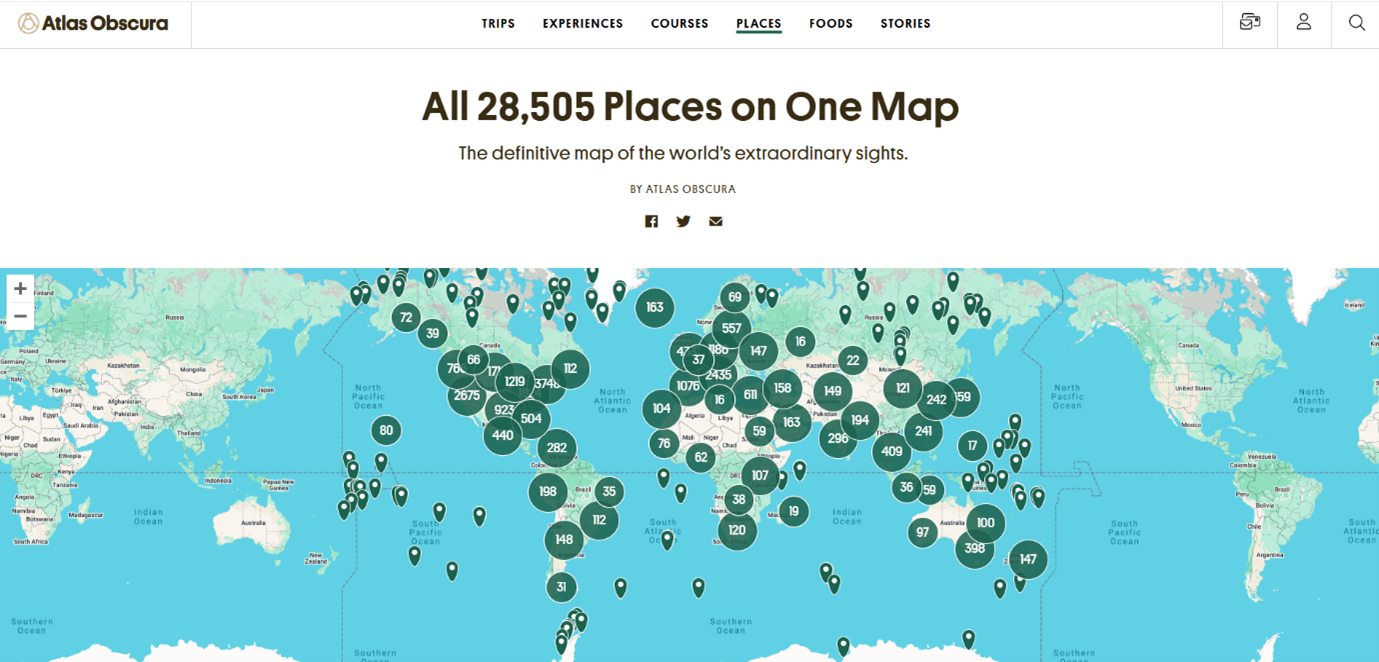
\includegraphics[width=\textwidth]{atlasObscura.png}
    \caption{Atlas Obscura places exploration}
    \label{fig:1}
\end{figure*}

The image shows the method the website has chosen to display all of the places that you
are able to visit, however circles showing things to do overlap, the same colour throughout
doesn’t attract the user to any certain locations, and there is no way for the user to get a gist
of the place or important information with ease from the website. All of this is poor human
computer interaction and will increase the cognitive load of the user due to the number of
options available and lack of guiding across the website. Another popular example is called
lonely planet. The website offered guides and information on all travel destinations around
the world. However the format that it is presented restricts or bores the user.

\begin{figure*}[ht!]
    \centering
    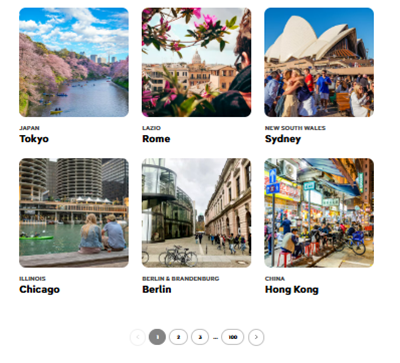
\includegraphics[width=0.5\textwidth]{lonleyPlanet.png}
    \caption{Lonely Planet exploration page}
    \label{fig:1}
\end{figure*}

A grid of 12 cities per page with over 100 pages to explore would cause the user mental
fatigue and there is a high probability that they would not go through all the designations
due to the format that they are presented. Therefore, the website has not done a good job at
presenting the information and options in the world. As well as lacking intuition or guidance
for the user to use their natural human urge for exploration.


\subsection{Milestones}
Weeks 1 to 4 in the predicted timeline where dedicated to the Travel Planner and has been successfully followed.
During this term datasets for every setting in the filters and radio filters have been implemented and mapped onto the globe. In addition, countries are all interactable and have some sort of data attached to them in the form of activities within the selected country.

Furthermore the itinerary generation has also been completed, once activities and countries are selected the user will recieve a planned out day by day itinerary, from arrival to departure, including information on transport and timings.

\scalebox{1}{
    \begin{tabular}{r |@{\bulletPoint} l}
        Week 1 - 2 & Add more datasets, make countries interactable and add more information \\
        Week 3 - 4 & Develop itinerary generation and finalize travel planner.               \\
    \end{tabular}
}
\section{Recipe App}
The Recipe Cooking App was created to tackle common challenges elderly people and visually
impaired users will face with cooking apps, such as cluttered layouts, small text and interfaces that require multiple actions that are unnatural to humans. This app streamlines the user experience by offering a simplified interface that begins with an customizable setup where the users can tailor the app to their specific needs. Overall this app helps users by reducing cognitive load, simplifying navigation, and enhancing visual clarity, ensuring that everyone can enjoy a smooth and engaging cooking experience regardless of demographic, age or abilities.
\subsection{Aims and objectives}
The aim of the app is to address accessibility challenges that the elderly and visually impaired users may face when using conventional cooking apps catered for the majority of users. The primary aim is to enhance the overall user experience by providing a clean interface that is easy to navigate without being overwhelmed and includes all user personas, meaning any challenges from bad eye sight to difficulty with certain colours should be mitigated. By offering customizable options such as adjustable font sizes and high-contrast colour themes, the app ensures that every user can tailor the display to their specific visual needs, thereby making the information more accessible and readable.

With the target audience in mind the app also needs to reduce complications and cognitive load by breaking down the cooking process into smaller steps through techniques such as decomposition. By breaking down the problem into smaller sequential problems all of the users will have a better experience navigating through the step by step format. This format will only allow users to focus on one task at a time reducing both intrinsic and extraneous cognitive demands while slowly completing the main task through many smaller ones.

\subsection{Motivation}
The second interface was created to tackle common challenges elderly people and visually impaired users will face with cooking apps, such as cluttered layouts, small text and interfaces that require multiple actions that are unnatural to humans.

The Cremes app is a cooking app which I found to be one of the best in the market currently in regard to human computer interaction. However it is not very inclusive, with a dark background and colour scheme which is fixed, some users may struggle to see the buttons which provide options. Multiple options in navigation from being able to swipe down and see multiple different categories as well swiping to the side to view recipes within those categories is too complex for elderly users that haven’t grown up with phones. Furthermore, some concepts may be unfamiliar to users who haven’t had experience with social media, such as the concept of posting stories.



\begin{figure*}[ht!]
    \centering
    \begin{minipage}[t]{0.4\textwidth}
        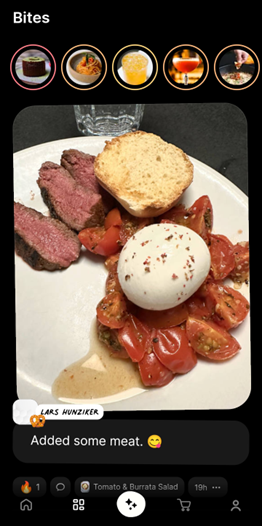
\includegraphics[width=20em]{cremeImage1.png}
    \end{minipage}
    \hfill
    \begin{minipage}[t]{0.4\textwidth}
        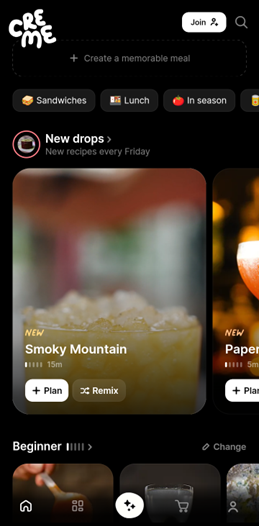
\includegraphics[width=20em]{cremeImage2.png}
    \end{minipage}
    \caption{Creme HomePage and recipe page}
    \label{fig:1}
\end{figure*}

With the sleek but packed interface cognitive load will not be reduced for the user which is negative as the aim is for the user experience to be as smooth and seamless as possible.
To improve I will be Aiming to enhance accessibility in cooking for elderly and visually impaired users through simplified navigation and a high contrast or custom palette design. Creating the objectives of designing a user-friendly login screen with large, high contrast text and customisable font sizes and colour schemes, giving the user options to enhance their experience. Next, I will implement a prototype for the recipe selection interface ensuring a clear layout, as well as simplify navigation by focusing on one instruction per page for clarity and usability.

A further issue with this app is its lack of clarity when it comes to starting the recipe, instead of following simple and coherent terminology such as start or begin they have chosen to use the word plan amongst the layout, this doesn’t stand out to the user and indicate an immediate call to action to them.

\begin{figure*}[ht!]
    \centering
    \begin{minipage}[t]{0.4\textwidth}
        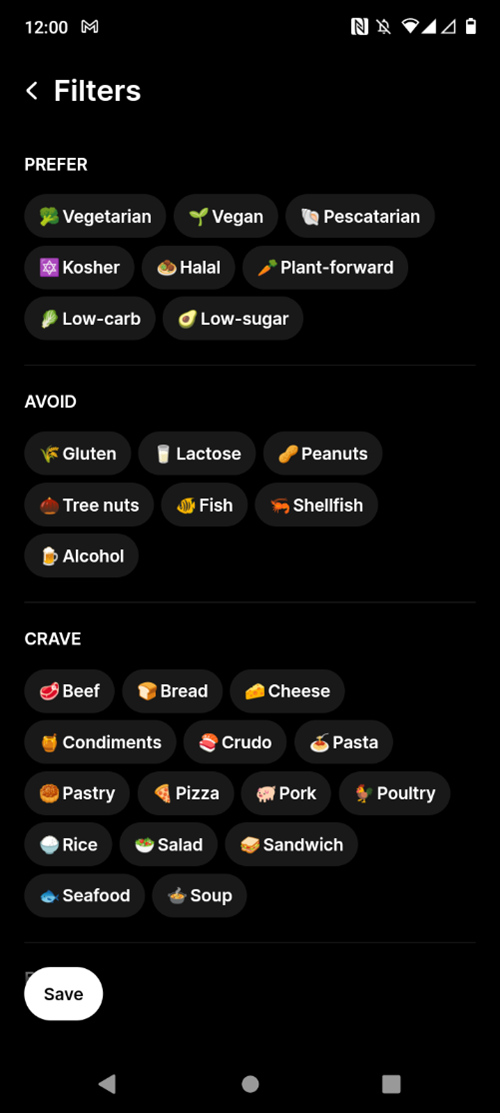
\includegraphics[width=20em]{cremeImage3.png}
    \end{minipage}
    \hfill
    \begin{minipage}[t]{0.4\textwidth}
        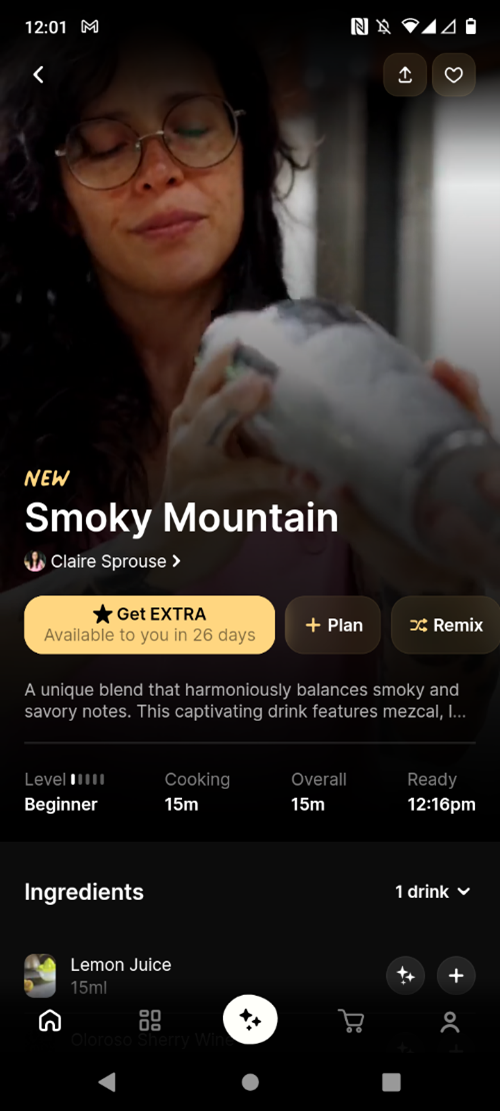
\includegraphics[width=20em]{cremeImage4.png}
    \end{minipage}
    \caption{Creme filters and selected recipe page}
    \label{fig:1}
\end{figure*}

Aspect of the application I did like was the user of icons throughout next to the text, this gives the user multiple forms of feedback on the screen. The consistency throughout the app is also something that I will be aiming for however with simplified interactions, and a better flow through the application inhibiting the user to wander off away from the task, which is: to select a recipe and follow it.

\subsection{Milestones}
The overall aim over the term was to provide and completed and tested app that enhances user experience and is inclusive to all users needs, specifically focusing on the elderly and visually impaired.

Terms 1 developement completed a basic structure to the app and provided alot of feedback for areas of improvement and personal preference.

Week 5 and 6 were dedicated to the further developement of the app, however this was not enough allocated space to act on all feedback and complete all tasks, hence why more time has gone into the app than anticipated.

The structure has been changed again, this time emphasising more images, bold characteristics, and memorable naviagtion in the form of tiktok style mechanics and accessibility tools.

Accessibilkiy tools have been implemented throughout in the form of captions, voice overs and a guided mode.

Following research the colour palette selector has also been changed, however the font size selector has been kept the same as it is adequate.

\scalebox{1}{
    \begin{tabular}{r |@{\bulletPoint} l}
        Week 5 - 6 & Act on supervisor feedback, change structure, add images \\
    \end{tabular}
}

\section{Art Gallery}
The Art Gallery was created to change the way users use and interact with online art galleries and e commerce stores. This was needed as the majority of online e commerce uses the same structure, meanwhile art galleries present all of their pieces in a symmetrical grid within borders and white backgrounds. This is neccessary for some pieces of work but does not represent others, or express the artist properly. By offering the user an immersive experience with artists and their art, and a smooth navigation to the checkout, the aim to increase conversation rates of sales online should be achieved, as well as increasing user engagemnt and task compeltion.
\subsection{Aims and objectives}
The aim of the Art Gallery is to engage the user and present the artists art in a manner which would translate their thoughts, feelings and emotions. This can be achieved through the structure of the page, strucutre of the navigation, or the colours used throughout. With this combination, creating satisfying and engaging pages with art that needs to be explored and can be purchased will keep the user on the site for a longer period of time, increasing the chances of a sale.

By creating different pages for the artists it will set them apart from one another, showing their personalities through methods that do not use vocabulary, instead using techniques that will make the user feel a certain way through compositions on the screen.
\subsection{Motivation}
The third interface identified a problem with the Online Art gallery Market, many platforms focus on transactions for business but neglect the user experience and the artists expression and presentation. Existing system often lack engaging visuals or clear navigation paths that would encourage exploration of different art.
Throughout research it seems that there is a common theme throughout the art galleries, all of the art shown is in grids with white backgrounds, and all of the artists pages are plain and simple with text and their work. This could be improved by connecting the user and the artist through their page, if the artist uses a certain colour palette, I will use that palette for the artist’s page. Different fonts could represent different people, clear and concise fonts would be a good depiction for architectural art while gothic or less coherent fonts would be suitable for abstract artists.

\begin{figure*}[ht!]
    \centering
    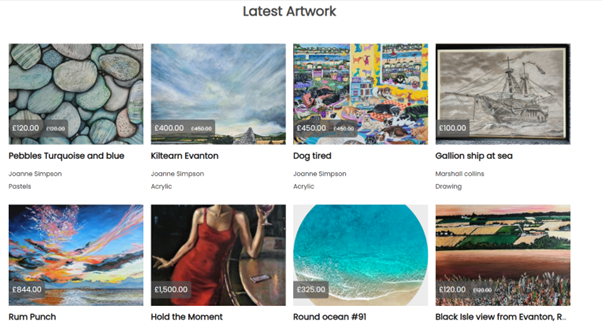
\includegraphics[width=0.4\textwidth]{artGalleryGrid.png}
    \vspace*{0.0cm}
    \caption{Example of online Gallery layout}
    \label{fig:1}
\end{figure*}

\newpage

Artsy is one of the largest online selling platforms of art in the world with a lot of information and content. To improve firstly we would need to simplify the website to show just necessary information and through progressive disclosure more can be revealed as per the users requests.
The next alteration I will make it creating the website more personal to the user and the page to represent the artist. Examples of good design for the user and artist have been shown below:

\begin{figure*}[ht!]
    \centering
    \begin{minipage}[t]{0.4\textwidth}
        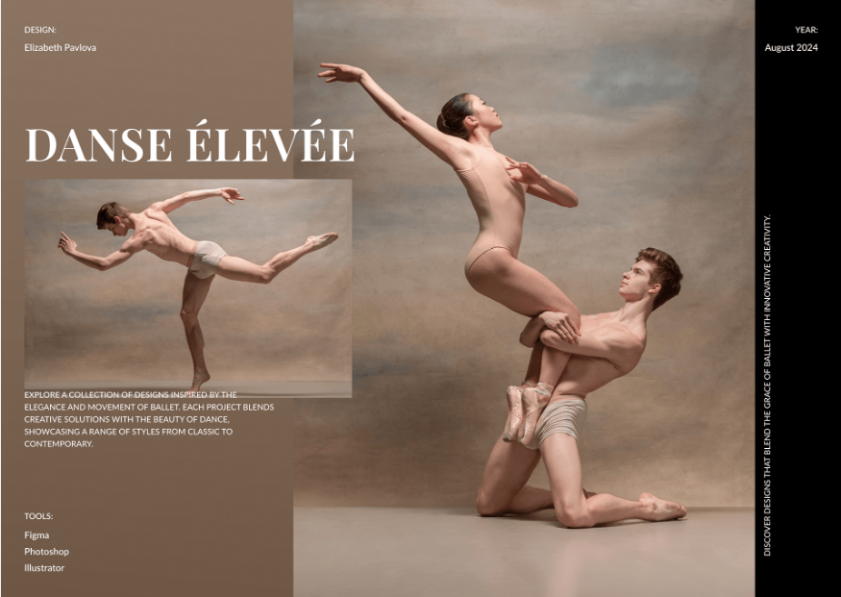
\includegraphics[width=20em]{artGalleryExample.png}
    \end{minipage}
    \hfill
    \begin{minipage}[t]{0.4\textwidth}
        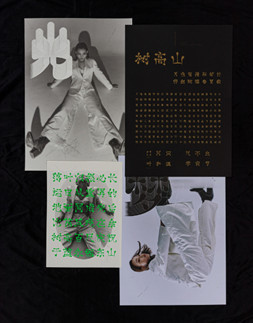
\includegraphics[width=20em]{artGalleryExample2.png}
    \end{minipage}
    \caption{Example of good layouts to showcase artists}
    \label{fig:1}
\end{figure*}
\subsection{Milestones}
In the first term wireframes where developed to outline the desired structure of my e commerce gallery, the aim for this term was to bring those wireframes to life.

I have exceeded this milestone, as i have created the wireframes and developed them into an interface, and then further added randomisation to the main page and completed all of the artists personal pages which reflected their work and styles correctly.

\scalebox{1}{
    \begin{tabular}{r |@{\bulletPoint} l}
        Week 7 - 8 & Develop interface based on wireframes \\
    \end{tabular}
}

\chapter{Background and Theory}
\section{Literature Review}
\subsection{Cognitive Load Theory}
Sweller developed the cognitive load theory during while researching how ”instruction design
interacts with the cognitive architecture of human memory”. The goal of cognitive load
theory is to optimize learning by managing the mental effort required to process information.
There are 3 components to the theory, long term memory, working memory and schema. The
working memory is responsible for the processing of information via either the visuospatial
subsystem which process visual and spatial information such as images and written text.
The other method is through the phonological subsystem which handles auditory and verbal
information such as speech. This theory directly relates with the design and layout of online
interfaces as the interfaces directly interact with the users working memory, if the interface
is poorly designed the working memory can be overloaded which would lead to frustration,
errors and abandonment by the user.
The theory identifies 3 types of cognitive load including intrinsic, extraneous and germane
load which all effect the user in different ways and have different methods of minimisation.\cite{de_jong_cognitive_2010}

\subsubsection{Intrinsic Load}
Intrinsic load is caused by the inherent complexity of the tasks that the users must perform
or the information that they must process on an interface. The load depends on the level
of interactivity which refers to the extent to which the user will understand the task. Tasks
with high interactivity are complex while tasks with low interactivity are simpler. However
the level of interactivity is dependant on the user and their past experiences which are stored
in the schema. For example, you had to translate a sentence from English to Spanish, the
task will be high interactivity for users that do not speak Spanish, however low interactivity
for users who speak both languages.
This has a big impact on the users as high intrinsic load can overwhelm the users which leads
to frustration and a higher percentage of errors. Or worst the user could not engage with the
tasks at hand and leave the interface. This is poor HCI as the aim is always to keep the user
engaged.
To ensure that intrinsic load does not cause negative impacts on the users there are many
methods to lower the load, for example breaking down the information of a larger task into
smaller and simpler steps for the user to follow. Another method would be to provide the
user with tools to guide them through certain tasks, such as templates or extra information.
Progressive learning is also a technique which is recommended and directly related to online
interfaces in my project. This is because progressive learning refers to isolating simpler
elements before showing the full complex task. For example, a filter button may hide a
modal screen with many filters available, but they are hidden behind the button to reduce
the intrinsic load for the user.\cite{de_jong_cognitive_2010}
\subsubsection{Extraneous Load}
Extraneous load refers to the cognitive effort caused by poorly designed interfaces and is
directly related to how the information is presented to the user. Cluttered layouts would
overwhelm the user with too much information displayed poorly for the working memory to
understand. Furthermore redundant content could force users to process unnecessary data
increasing the load.
Increased extraneous load increases the users mental effort without helping towards the task
completion and can frustrate users which causes a higher percentage of errors to be made
during the tasks.
To reduce the extraneous load the design of the interface should be simplified , clean and
uncluttered, this means that any data or information that is obsolete or not needed should
be removed as well as duplicated. Another way to reduce would be to follow common design
principles for interfaces such as visual hierarchy and Gestalt principles to guide the users
attention correctly.\cite{de_jong_cognitive_2010}
\subsubsection{Germane Load}
Germane Load refers to the mental effort needed for learning and understanding and developing our schema. This is considered a positive load and we want to be able to increase
it to the maximum without effecting the intrinsic or extraneous load. It is crucial in how
interfaces are structured as the load helps recognise patterns, apply concepts and learn new
information without any prior knowledge. This is because it focuses on active learning and
pattern recognition and is stimulated by tasks such as connection past experiences to new
information which highlights why interfaces must be kept consistent throughout as the user
is constantly learning how to interact with it and recognising patterns.
The Germane load is increased when the user is included in interactions such as tutorials
or challenges. Prompts to engage the user or focus attention would be equally as effective.
Another effective strategy is to reinforce patterns by using consistent layouts and symbols to
enforce learning and interaction as the user becomes more comfortable on the interface.\cite{de_jong_cognitive_2010}
\subsection{Progressive Disclosure}
Progressive Disclosure is a principle that reveals information gradually to the users, managing cognitive load by revealing information incrementally rather than presenting all available information or options at once. This technique ensures that users can focus on their immediate task presented without feeling overwhelmed by excessive information or options. Research shows that too much transparency or immediate access to all features and information can lead to decision fatigue and distraction which would prevent the user from completing simple tasks to progress the interaction.\cite{uxpin_what_2023}

The goal of progressive disclosure is to show information in a structured manner, when it is needed. This created a better experience for the user as they are being guided through the program to reach the information they are searching for. This is very effective in complex systems where users have multiple options to choose from but do not need all of the information at the same time.

Cognitive Psychology suggests that users process and retain information better when it is presented progressively. Progressive disclosure aligns with the Cognitive Load Theory by reducing extraneous load and ensuring that only relevant information is presented to the user. A study by bailey et al. demonstrated that users complete tasks 27 percent faster when interfaces use progressive disclosure in contrast to presenting all of the information and options at once.

An advantage of this principle is its ability to optimize information hierarchy. Instead of displaying an overwhelming list of options, progressive interfaces prioritize key actions, allowing users to learn and navigate the system naturally. For example, a step-by-step filtering process in digital interfaces can reduce decision complexity and prevent unnecessary distractions.

Many studies have been conducted in usability research and have consistently shown benefits of progressive disclosure and its ability to improve the user experience, decision making and task efficiency. Its biggest advantage is its ability to reduce decision fatigue, this is where a user is overwhelmed when confronted with an excessive amount of choices at once. Schwartz found out that users who were presented with too many options had a higher cognitive strain, leading to increased abandonment of tasks and poor decision making if the user completed the task. However, in contrast, the interfaces that were designed with progressive disclosure had lower abandonment rates as users were able to navigate the options correctly and incrementally rather than being confronted with an excessive amount of options and choices at once.

As much as progressive disclosure reduces cognitive load, it also improves learning and task efficiency. Mayer and Moreno conducted a controlled study on digital learning systems. The study showed that progressively disclosed interfaces led to a 40 percent increase in task completion. The study said this improvement was due to the improved structure of information. The structure also presents the information in a way for the user to more easily process the information and remember more. The findings show how important progressive disclosure is when users need to interact with information, multi step processes or complex datasets.

Progressive disclosure is relevant to planning applications such as the Travel Planner due to its structured filtering mechanisms and the way information is presented in multiple layers. Many different methods of progressive disclosure can be used, for example, the Travel Planner uses step by step filtering where the user has to select a Travel month first and then gets the option of additional filters. Zoom based information control to dynamically adjust which markers are relevant on the screen at certain zoom levels.\cite{springer_progressive_2019}

\subsection{Colour Theory}

Colour Theory refers to how colours interact and influence human emotions, perceptions and behaviours. Within human computer interaction colour plays a big role in interface design as it can be used to show user information, guide them throughout or enhance accessibility. Colours can also effect how the user perceives the content, for examples certain colours or combinations could infer trust, usability and engagement to the user through triggering subconscious responses that will influence the user decision making and perception.\cite{interaction_what_nodate}

\subsubsection{Psychological and emotional impacts of colour}

Humans have an instinctive response to colours. Warm colours such as red, orange and yellow would represent warmth while cool colours such as blues, green, purples would represent cold areas or cooler parts of the world. However there are many representations for colours within contextual scenarios, for example, red can raise heart rates and grab attention as it is associated with emotions like anger or passion, therefore relating to danger and danger signs. In contrast Blue is a colour associated with trustworthy. Through studies conducted, it is shown that lighter blues produce calming effects while darker blues feel more confident and authoritative. Green is often linked to nature and tranquillity which aids stress relief. These emotional effects are so reliable that they have real world application in things such as branding of companies. Fast food restaurants use energetic colours such as red and yellow to stimulate the audiences appetite, such as MacDonalds.\cite{inbook}

Colour can also influence decision making unconsciously. Research within psychology showed that even subtle colour cues impacted task performance. A study had participants working with a red background performed 31 percent better on detail oriented tasks than those that had a blue background. However participants with a blue background had a doubled creativity output compared to the red participants. This is because sub-consciously re is associated with danger and caution, for example stop signs, this triggers focus to avoid the danger. Blue is associated with the sky and openness which creates a explorative mindset that encourages creative thinking.\cite{elliot_color_2015}

Colours can also regulate the mental effort required to process information. Interfaces with too many clashing colours demand more cognitive processing which could overwhelm users. By simplifying the colour palette it would help the user focus on information and reduce cognitive load. For example, neutral backgrounds with one bold main colour that contrasts for important buttons will allow users to quickly recognise actionable elements on the page. Research shows that a suitable colour contrast can boost readability by up to 40 percent which would lead to fewer errors from the user. This means that the right colour choice for the interface has the ability to guide the user into a certain emotional or cognitive state that the program wants.

Valdez and Mehrabian conducted research to see how colours effect emotions and judgements. They found that people tend to rate brighter and more saturated colours as pleasant, and consistently reacted to colours in the same way, for example blue and green tones for calmness. This is where the idea that colour can affect the emotions and judgement came about.\cite{article}


\subsubsection{User Perception of colour}

Users interpret colours, their meanings and the expectation they have from seeing the colour on individual elements. Online red is perceived as a error indicator in error messages or delete buttons. Green on the other hand shows the user their process has been successful or provides a confirmation screen in the form of a valid checkmark or any other positive connotations. Blue is commonly used for hyperlinks and interactive elements because in the early web users would associate blue with reliable interactivity. By understanding the way users interpret colours we can understand a lot of conventions within interfaces. For example, when a form field highlights red the user will be able to see that there is an error without extra explanation, or a green success message that would confirm completion of the form.

Colour, saturation and colour harmony are important in lead design choices. Contrast between text, icons and background is critical for clear readability for the user, for example, dark grey text on a light background is better for the eyes than pure black text on a white background and the grey still keep the clarity and contrast for the user. WCAG guidelines suggest 4:5:1 contrast ratio for normal text, this would ensure that the content is legible for most users. Furthermore, saturation, which refers to the intensity of the colours used, can be used throughout the interface to emphasis centre parts or information as it draws the eyes to that area. A bright saturated colour such as a bright orange "Buy Now" button will draw the users eye to the call of action button. However highly saturated colours can be overwhelming, therefore interfaces create visual hierarchy through mixing a dominant neutral tone with minimal saturated colour to make elements stand out.

Achieving colour harmony means combining colours in a visually appealing way often through the use of classical colour schemes. The colour harmony palette helps the user concentrate on the content rather than distract the user. Good harmony support usability of the interface by providing consistency as users learn to associate certain sections of functions in the interface with certain colours. By creating this consistency throughout, the interface becomes to feel intuitive to the user as all of the colour cues are logical. This reduces the mental effort needed to interpret the interface which would improve the user experience.

Studies that have been completed on usability support these principles and theories. For example, one study found that colour coding sections of a complex website reduces the task completion time by 30 percent as the users could skip to the section identified by a specific colour. This increases navigation speed. Similarly, suitably contrasting interface elements aid readability and lower the user error rate throughout the interface.\cite{colour_what_nodate}

\subsubsection{Cultural Variations in Perception of colour}

The meanings of colour and their harmony however is not universal, they vary widely across cultures. This means interfaces must be careful with the palette selection as colours that represent something positive in one society may represent negative emotions in another. For example the colour Red. Red has connotations to danger and errors within western society, in contrast Chinese culture views red as a symbol of luck and prosperity and is widely used in events with positive connotations such as festivals and weddings. This different view of the colour could cause issues within interfaces as an interface element coloured red in a Western app might signal “stop, something’s wrong,” whereas a red accent in a Chinese app could seem celebratory or positive. The west view the colour white as positive, it is used in weddings and is associated with cleanliness and purity, however parts of east Asia such as China, Korea and Japan use the colour white to symbolise mourning and death.

%When designing interfaces cultural adaptation is necessary if the interface is for a global audience, this is so that the correct message and meanings are conveyed. For example, A notable case study is Pepsi in Southeast Asia, when Pepsi changed its vending machines to light blue, which is a colour seen as refreshing in the west, they didn’t realize that light blue is associated with mourning in that region. The result was a sharp drop in sales until Pepsi reverted to a more culturally neutral colour​.

Adams and Osgood and Hupka et al both studies cultural colour associations across 23 nations. Throughout they found that blue, green and white were perceived as positive across most countries, especially in the west, and red was universally linked to strong emotions. However these emotions have a wide range of meanings from danger in the west to good fortune in China. This means that colours should be localised for the cultural expectations if the interface is worldwide.\cite{inc_how_2020}

\subsubsection{Task Performance and cognitive load}

Colour plays a vital role in affecting both task performance and cognitive load as different colours influence attention and focus which would guide how the user interfaces with the interface. Studies suggest that warm colours are more attention grabbing than cool colours which promote concentration and cognitive persistence. Stone found that many user interfaces in red improved reaction speed by 12 while blue interfaces increased task endurance. Similarly, chaparro et al showed that participants completed visual search tasks 20 percent faster when high contrast colours were used foro key information which shows that colour can reduce search time and increase efficiency for the user within the interface.

However it is not only the colour that plays a effect , it is also its contrast. The contrast affects the task completions and user accuracy of tasks in the interface. This is because high contrast schemes help the user find the key information faster, while low contrast combinations would increase the reading effort for the user and slow down finding the key information. Hill and Scharff found that users reading black text on a white background had the fastest reading times, whereas low contrast colour pairs increased reading times by 30 percent. Bauer and Cavonius also discovered that interface elements with a  contrast ration of 4:5:1 led to 38 percent less errors. This shows that the interface needs a well balances contrast to be optimal for the user.\cite{colour_readability}

\subsection{Accessibility}
Accessibility design is important because it ensures that digital interfaces are usable by a wide range of individuals with different abilities including visual, auditory, motor and cognitive impairments. By enhancing accessibility for all users the interfaces would increase usability, user retention and inclusivity. This would give the interface or company a larger audience. Accessibility guidelines are in place such as the Web Content Accessibility Guidelines (WCAG) which set global standards for design inclusivity. Accessibility is also a legal requirement in many countries from the United Kingdom who have the equality act (2010) or the United States who have the Americans with Disabilities Act (ADA).

\subsubsection{WCAG accessibility standards}

The first is Perceivable, this means that all users can perceive the content presented regardless of visual or auditory ability. For example, images should have alternate text, videos should have captions, and text should be high contrast to enhance readability. Lazar et al found that implementing alt-text descriptions improved navigation speed of visually impaired users by 35 percent.

The second is operable, this means that the user must be able to interact and navigate the system. For example, there should be multiple options from keyboard navigation, voice commands and adjustable time limits for interactions.  Babu and singh found that keyboard accessibility increased task completion by 28 percent in users with motor impairments.\cite{babu_understanding_2010}

The third is understandable, this means interfaces should be predictable, intuitive and easy to understand. This would include the interface having readable fonts, simplified workflows and consistent navigation structures. Gargiulo et al showed that clear interfaces reduced cognitive effort in users with dyslexia by 40 percent.

Finally, the fourth is robust, this means that content must be compatible with assistive technologies and different devices. For example being screen reader support compatible, and compatible with different environments.\cite{noauthor_web_nodate}

\subsubsection{Importance of accessibility}

Accessibility is not only important because it helps the user but also because there are many legal obligations for companies in place. Law and regulations ensure accessibility in digital platforms through acts such as the Americans with Disability Act (ADA) or Equality act or European Accessibility Act (EAA). Companies working under the acts must comply or risk facing financial penalties, legal action or reputational damage to the company or interface.\cite{gada_importance_nodate}

In 2019 Dominos Pizzas was taken to supreme court in the United States due to failing to comply with the Americans with Disability Act. This is because they failed to make their website accessible for visually impaired users.
Another example is Netflix. They were sued in 2012 for failing to provide captions for hearing-impaired users which lead to a financial penalty and mandatory changes and
improvements to accessibility.\cite{higgins_supreme_2019}

Furthermore, being accessible allows your interface or brand access to more customers. 15 percent of the global population live with some form of disability according to the world health organisation. This is a large market that would be left untouched for businesses if accessibility is not considered. In 2021 Microsoft implemented accessibility features which increased user retention by 25 percent. Another study showed that accessible websites see a 20 percent increase in sales conversions due to improved usability for all users.

\subsubsection{Different types of accessibility}

The visually impaired face many challenges such as difficulty reading small text, distinguishing colours and interpreting images. This includes over 2.2 billion people across the globe which all suffer from some form of visual impairment.
Implementing High contrast colours to improve readability is supported by Bailey et als studies. They found that high contrast interface elements improved readability by 32 percent. This means that interfaces should have multiple options such as dark mode for users with light sensitivity and allow customisable contrast settings or colour palettes.\cite{noauthor_web_nodate}

Some users suffer from motor impairments, which means they could have a difficulty using precise cursor movements, mouse clicks or complex gestures on devices. Furthermore, users with cerebral palsy and Parkinson's may rely on alternative input methods.
It is best to implement keyboard navigation and shortcuts, this is supported by Babu and Singhs study which found that keyboard accessibility increased task completion by 28 percent.
Another method to include these users is through voice control methods. Dragon NaturallySpeaking research found that voice navigation improved efficiency of users by 24 percent.\cite{babu_understanding_2010}

Not all challenges for the user are visible, for example ADHD, dyslexia and memory impairments which could make complex layouts overwhelming. Garguiulo et al found that simplifying navigation reduced cognitive strain by 40 percent. To make layouts simpler the interface should be a structured navigation and have readable fonts. Suk and Irtel found that sans-serif fonts improved readability by 30 percent . Another method could be using Progressive Disclosure to gradually reveal content, information and options. Mayer and Moreno found that the gradual reveal of content improved task performance by 27 percent.\cite{sans_serif}




\subsection{Visual Hierarchy and Eye Tracking}

Visual Hierarchy and eye tracking are concepts that are user in the interface to create a better user experience. Together they explain how users interact with visual content and navigate interfaces through studies which track the human eyes natural behaviour when interacting with a interface. Understanding the principles of visual hierarchy and the eye tracking studies will lead more efficient interfaces which better cater to the users needs.

Visual Hierarchy refers to the arrangement of elements on the page to guide the user in a structured manor. This means that the user will be directed to the most important information first as well as understand relationship or connected content and components in the interface.\cite{visual_heirarchy}

According to Djamasbi, visual hierarchy determines the sequence in which the user will
process content on the screen. Effective Hierarchy focuses attention and reduces cognitive
load. The sequence can be impacted by many different principles such as:
Size - Larger elements on the interface will attract more attention as demonstrated by
Faraday who conducting an experiment on directing search behaviour with size.
Contrast - High contrast between elements makes the content easier to read and understand.
Colour - Vibrant or bold colours enmphasis specific elements while muted tones will go into
the background.\cite{djamasbi_visual_2011}
Positioning - Lavie and Tractinsky showed that central placement often correlates with user
engagement due to a natural gaze pattern from user behaviour.

Eye tracking is the measurement of eye movement to understand how users will interact
with interfaces. It shows the natural flow of user attention and identifies which part of the
interface capture the most attention. This can help with optimising the layout of an interface
to improve usability and the user experience. The Nielsen Norman Group found that users
follow similar predictable patterns such as the F-pattern or the Z-pattern which were found
via heatmaps which reveal ”hot zones” where attention is concentrated such as the central
and upper left areas of the page.\cite{eye_tracking_nn}

\subsection{User Experience}
User experience refers to a users overall feelings and perceptions of the interface when interacting with it. The international standards organisation (ISO) defines user experience as a person's perceptions and responses that result from the use or anticipated use of a product, system or service”.

Good user experience design manages cognitive load. To do this the interfaces need to be simplified and align with users mental models to prevent overload. For example Hicks law and Fitts Law are applied to interaction design to be able to streamline the users actions. Fitts law states that the time to move to a target, in this case a element for example a button on the screen, depends on the distance to the target and its size. This means interfaces can make targets that are more important larger and closer on the screen.\cite{hicks_law}

\subsubsection{Impact on User engagement and efficiency}

The Nielsen Norman Group reported after they focused on usability the users task success rate and conversions increased by an average of 135 percent. This shows that features such as an undo or back option are significant as they reduce task completion times and user errors.

Google differentiated themselves with a clean and minimalistic homepage which set them apart from other search engines who had adds and selections of categories.  Another example of a company who makes their app through user research and iterative design to achieve the best user experience is Airbnb. They redesigned the app and its navigation to make it hierarchical and visual with labels such as "Homes" and "experiences" which allowed users to find what they were looking for faster and increasing booking rates.

\subsection{Information Architecture}

Information Architecture Refers to the structural design of information on the interface, how the content is organised, labelled and arranged. This determines how quickly the user is able to navigate and find the information that they need. To make this easier information should have a logical hierarchy with categories and labels. A good interface will have information grouped intuitively using familiar conventions which allows users to search confidently throughout the interface and not feel lost. however a poorly structured site may have information scattered and force the users to use more cognitive effort to find what they need. This often leads to abandonment of the interface due to frustration and reduces engagement.\cite{information_architecture}

\subsubsection{Real-World Examples}

Search engines such as Yahoo! had a complex hierarchy of topics that users had to click through to navigate, in contrast Google offered a singular simple search box that algorithmically organised the web for the user. This made information accessible through key words which improved the speed of navigation.


\subsection{Emotional Design}

Emotional design refers to how an interfaces makes the user feel. This is done through a wide range of elements from colour, imagery, typography, shapes and animations. These will form aesthetics within the interface and make the user feel a certain way, by provoking emotions such as happiness, trust, frustration or surprise for example, it affects the users feelings towards a product or information. Colours carry phycological connotations that can be used in different circumstances.\cite{noauthor_what_nodate}

Similarly, typography and the layout can influence a users emotions. A cluttered layout with hard to read text could induce stress and frustrate the user, while generous white space and a clean font can make a user feel relaxed. This extends to subtle details, for example, rounded corners on buttons feel more friendly and inviting than sharp corners which feel more efficient and formal. This would convey the products tone online.

\subsubsection{Normans Emotional Design Framework}
The Emotional Design model breaks down the user experience into 3 levels: visceral, behavioural and reflective. At the visceral level the users reactions are instinctive and refer to how the user reacts to the interface, its look and feel, at first glance. It usually focuses only on appearances and is the users first impression. For example, seeing a visually appealing hero page or load in page to the interface will evoke a positive response through the user instinctually.\cite{komninos_normans_2020}
The behavioural level relates to the effectiveness of the product. Does it feel easy to use and accomplish set tasks? The emotions at this level arrives depending on how the interface or product behaves.
The reflective level is the highest level as it involves conscious thought. This is because it touches on peoples personal experiences and emotions such as pride, nostalgia or sense of trust in that interface.

Norman suggests that designers should address all three levels to create a good experience for the user as his model is supported by research which states that first impressions are formed by the user within the first 50 milliseconds. Interfaces which are meaning full to the user (reflective) are cherished longer, however to get to that stage the user must be engaged with the visceral level, meaning that the aesthetic must be good looking instantly.\cite{noauthor_3_nodate}


\section{Technology choices}
The Travel Planner was developed in the svelte framework which is ideal for building reactive web applications. It was also chosen for its good performance and minimal runtime JavaScript.
The Mobile Recipe App was developed in the flutter framework as it provides a "hot reload" feature that allows me to quickly view changes and refine the app to my needs quickly and efficiently.
MapBox was used to power the 3D Interactive globe as it supports layers  and styling of the globe, as well as providing documentation and guidance in languages such as svelte help me start off the project.
Turf.js is a geospatial analysis library that is used to calculate distances and similar geographical operations. In my project I needed to calculate the area of a country and map its borders to be able to map colours and layers within restrictions outside of the.
Hugging Face interface API has been used due to its easy setup and minimal requirements in comparison to other APIs such as chatgpt which requires python integration and uses more tokens.

The Dart language is also an intuitive language that is easier to pick up in comparison to other language due to it structural approach. This along with extensive documentation online made it and the flutter framework chosen for my app.

The Art Gallery was created in svelte due to its increased performance and simplified state management. Furthermore svelte is a very intuitive framework for web development with a low learning curve, making it easier to learn and implement in my work. I needed complete control over the designing of the webpage, hence why I used Vanilla CSS rather than frameworks.

\chapter{Implementation}
\section{Travel Planner}
The Travel Planner is an interactive web application that has been created with the aim
of simplifying the process of exploring Travel destinations around the world. It provides
essential travel data to the user progressively through techniques such as progressive disclosure and colour theory to reduce the users cognitive strain in the process of navigating and understanding the information.

\subsection{Initial Screen}
\subsubsection{Globe Placement}
The initial design of the Travel Planner is structured to ensure an engaging experience and provoke user interaction with the interface. This interface focuses on many techniques from progressive disclosure to visual hierarchy that will ensure that users gradually interact with the system without being overwhelmed.

The globe is positioned centrally within the interface as it is the primary interactional element. Following Gestalts principles of central focus, he states that users attention naturally gravitate towards the centre of the screen. This is reinforced by eye tracking studies completed by Djamasbi et al who found that users start scanning the interface from the centre and top left parts of the screen in most interfaces.

\begin{figure*}[ht!]
    \centering
    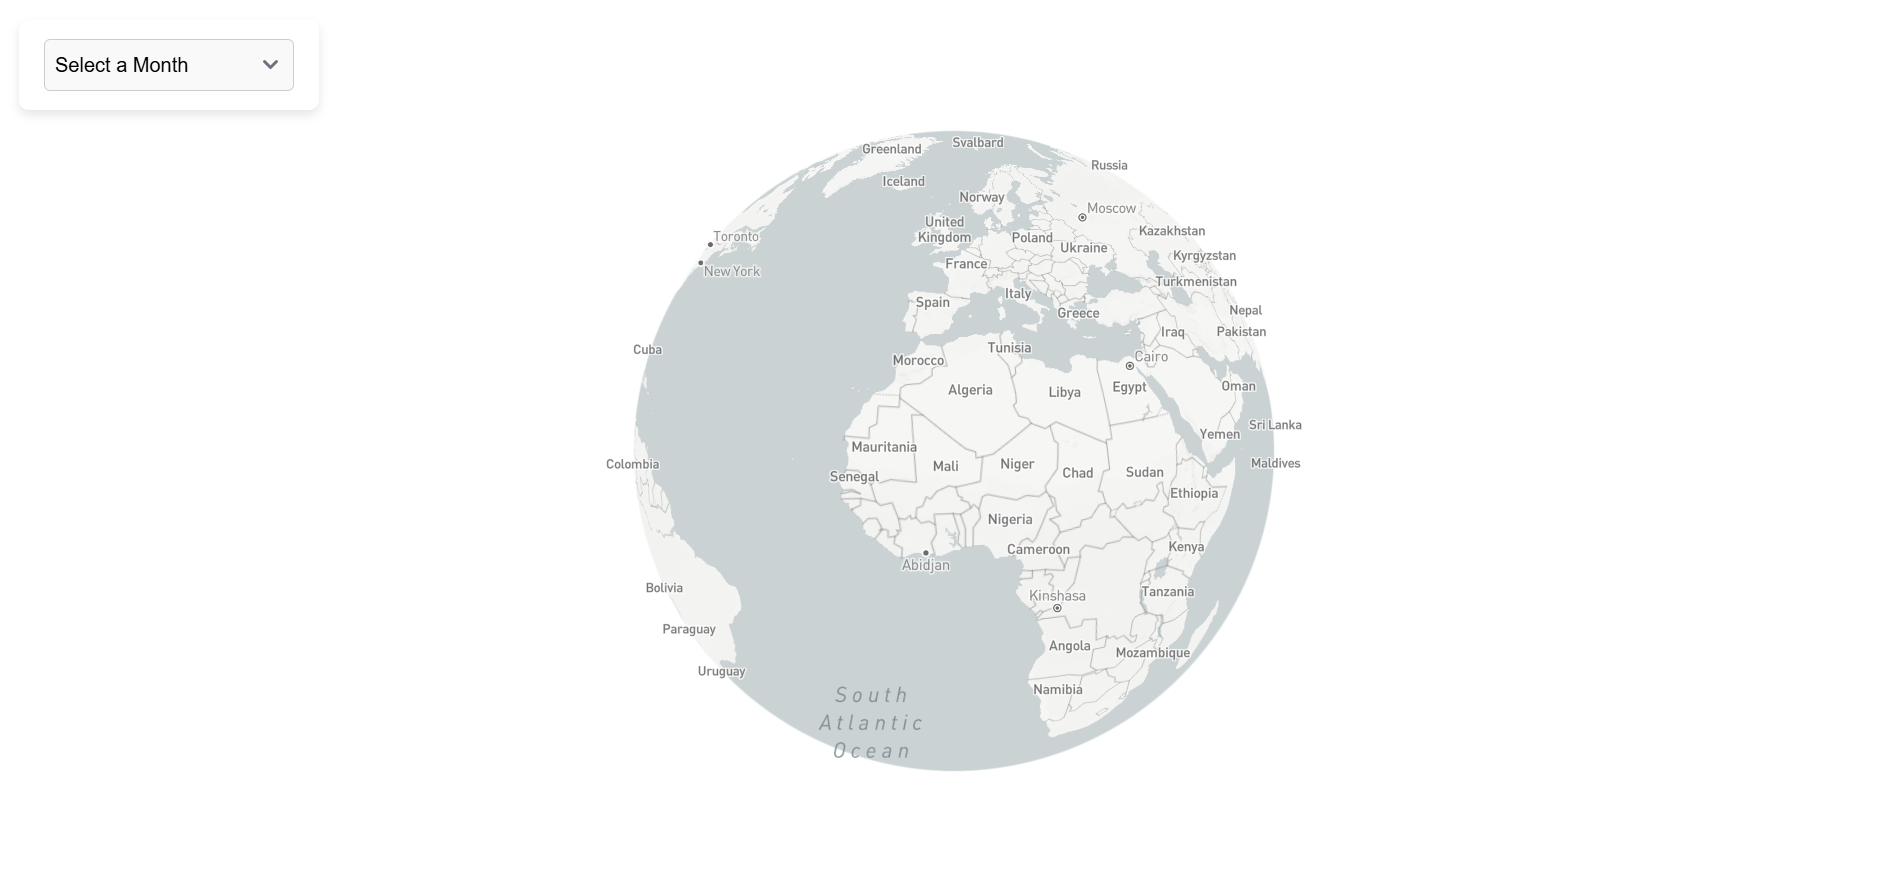
\includegraphics[width=\textwidth]{1.png}
    \caption{Central Placement of the Globe}
    \label{fig:1}
\end{figure*}

The globe as a focal point within the interface ensures that users immediately recognize it as the primary interactive element. This is confirmed to the users through the large scale of the globe and minimal distractions to prevent decision fatigue. The lack of other elements throughout this page avoids clutter and ensures that the users focus on the geospatial information.

\subsubsection{Button placement}

The dropdown menu is in the top left for many reasons, firstly, Nielsen found that users start scanning from the top left, this ensures that the first action they see if selecting a month. This runs in accordance with research in the F-Pattern reading flow.

To reduce cognitive load only one clear option is available to the user. This doesn't overwhelm them and is called progressive disclosure. This is because the user is guided step by step through the selection process as additional filters only appear once a month is selected.

\begin{figure*}[ht!]
    \centering
    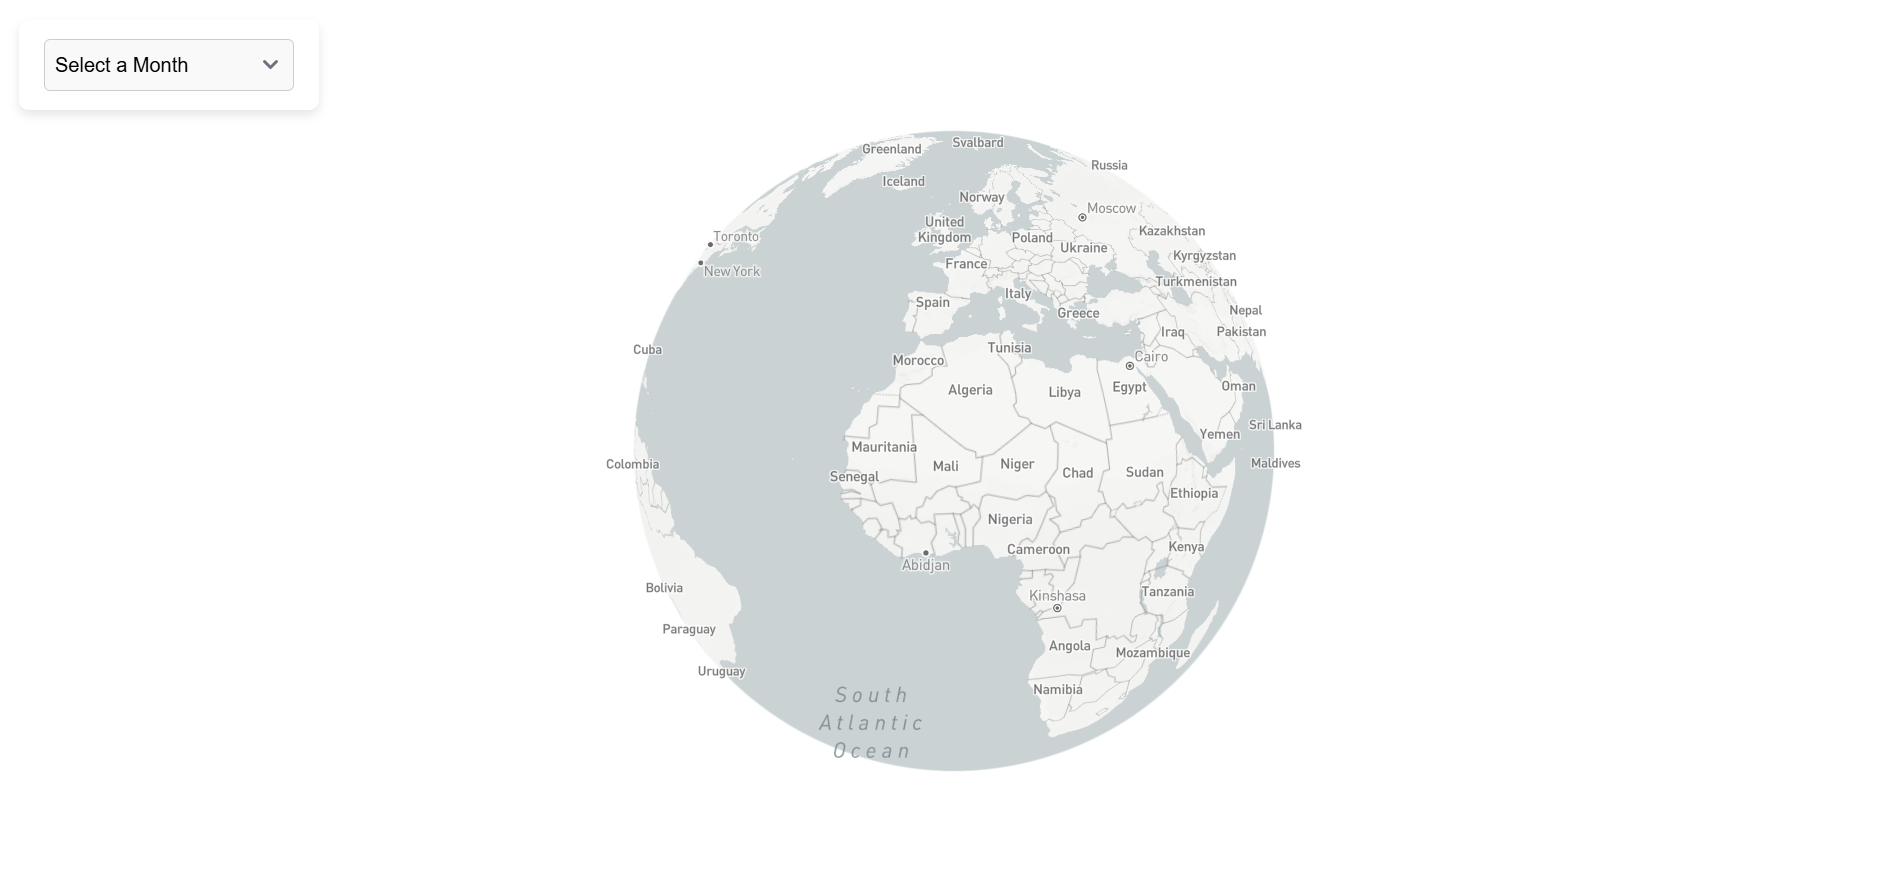
\includegraphics[width=\textwidth]{1.png}
    \caption{Filters in the top left following F-Pattern Design}
    \label{fig:1}
\end{figure*}

The filters button has round corners as they align with emotional design principles. Norman conducted a psychology study which found that soft and curved edges create a more friendly user experience as they are less intimidating and create a welcoming atmosphere.  Furthermore, sharp corners are usually seen in professional settings, such as a website for lawyers or financial advice as they are serious topics.

\begin{figure*}[ht!]
    \centering
    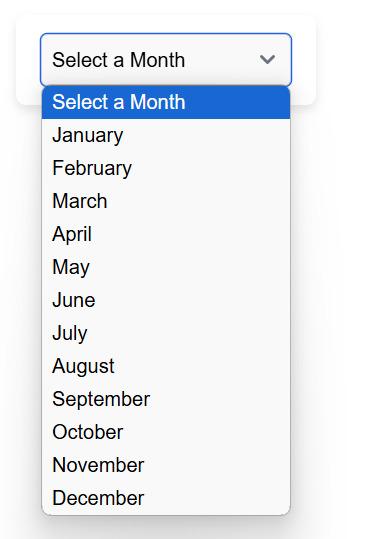
\includegraphics[width=.5\textwidth]{2.png}
    \caption{Progressive Disclosure example when user selects the filters}
    \label{fig:1}
\end{figure*}

\begin{figure*}[ht!]
    \centering
    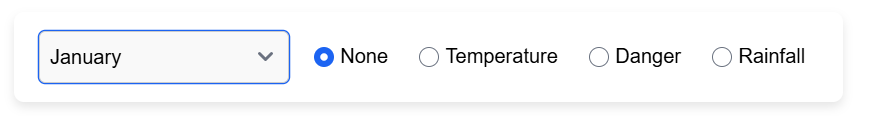
\includegraphics[width=\textwidth]{3.png}
    \caption{Progressive disclosure example when a user has selected a month}
    \label{fig:1}
\end{figure*}

Only one button is used to ensure that the users do not feel overwhelmed at the start of the interaction. Furthermore the progressive disclosure and gradual interaction keeps the users attention and engages them while reducing cognitive strain. Further filters such as temperature, safety and rainfall will only appear when they become relevant in the decision making process which maintains a smooth user experience.

\subsubsection{Travel month selected}

Colour coded overlay uses a gradient scale to represent different datasets. The colour of the gradient is selected through the previous associates the user will have with colours intuitively. Cyr et al showed that colours influence user perception and usability. For example, if the temperature dataset is represented the gradient used would be from warm colours to cool colours.

Warm hues are associated with heat, so red and orange will represent hotter regions on the globe in that month.

Yellow will represent mild warmth as the colour will be a visual transition to the user from the hot and cool areas.

Cooler tones will represent lower temperatures which will align with the users expectations, so the colour blue and green will be used for the colder regions.

\begin{figure*}[ht!]
    \centering
    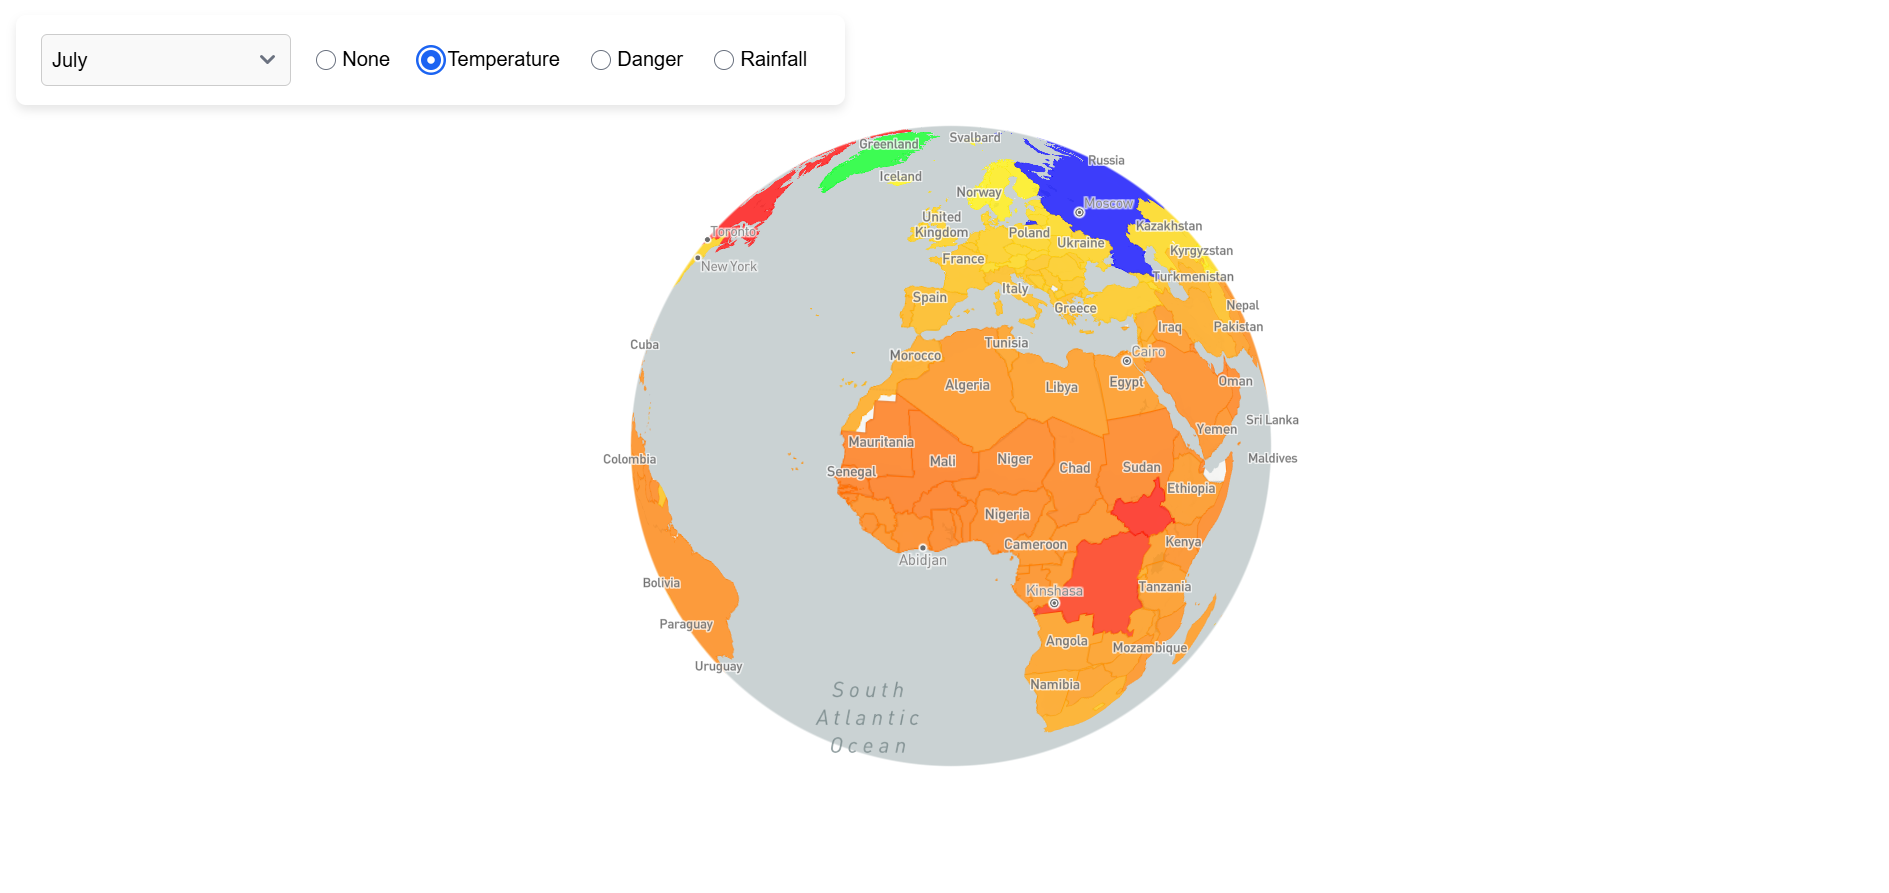
\includegraphics[width=0.4\textwidth]{4.png}
    \caption{Temperature dataset visually represented in July}
    \label{fig:1}
\end{figure*}

\begin{figure*}[ht!]
    \centering
    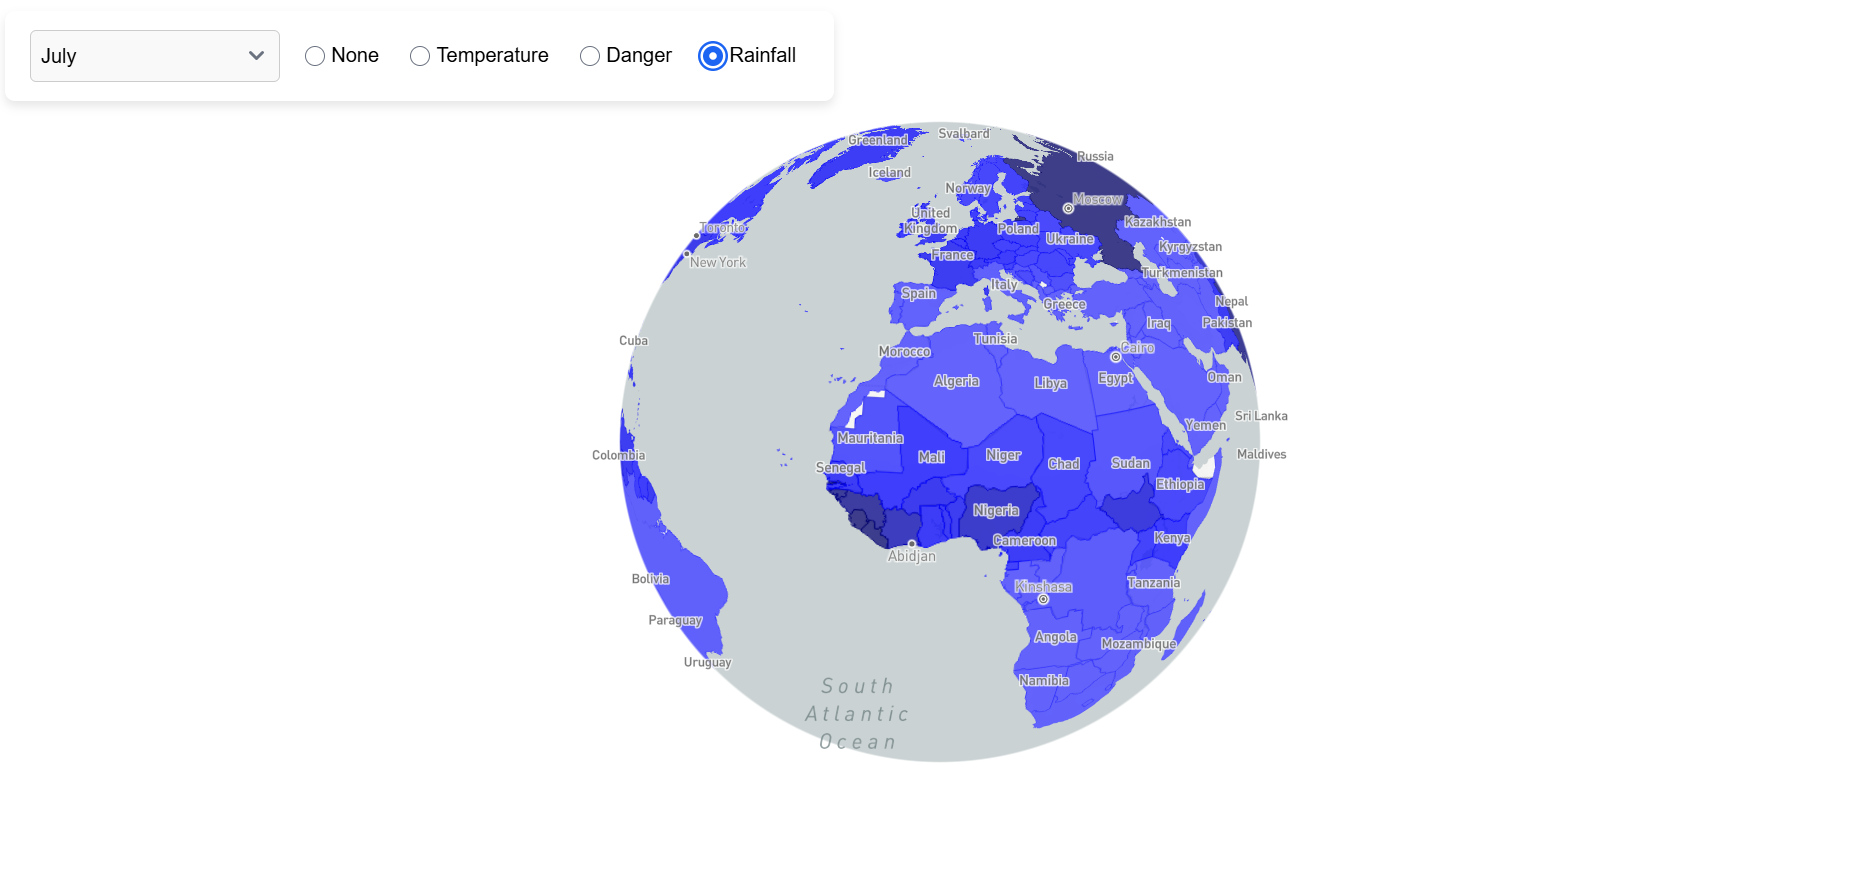
\includegraphics[width=0.4\textwidth]{5.png}
    \caption{Rainfall dataset visually represented in July}
    \label{fig:1}
\end{figure*}
Rainfall is represented in a blue gradient due to humans natural association with the colour blue and water.


\begin{figure*}[ht!]
    \centering
    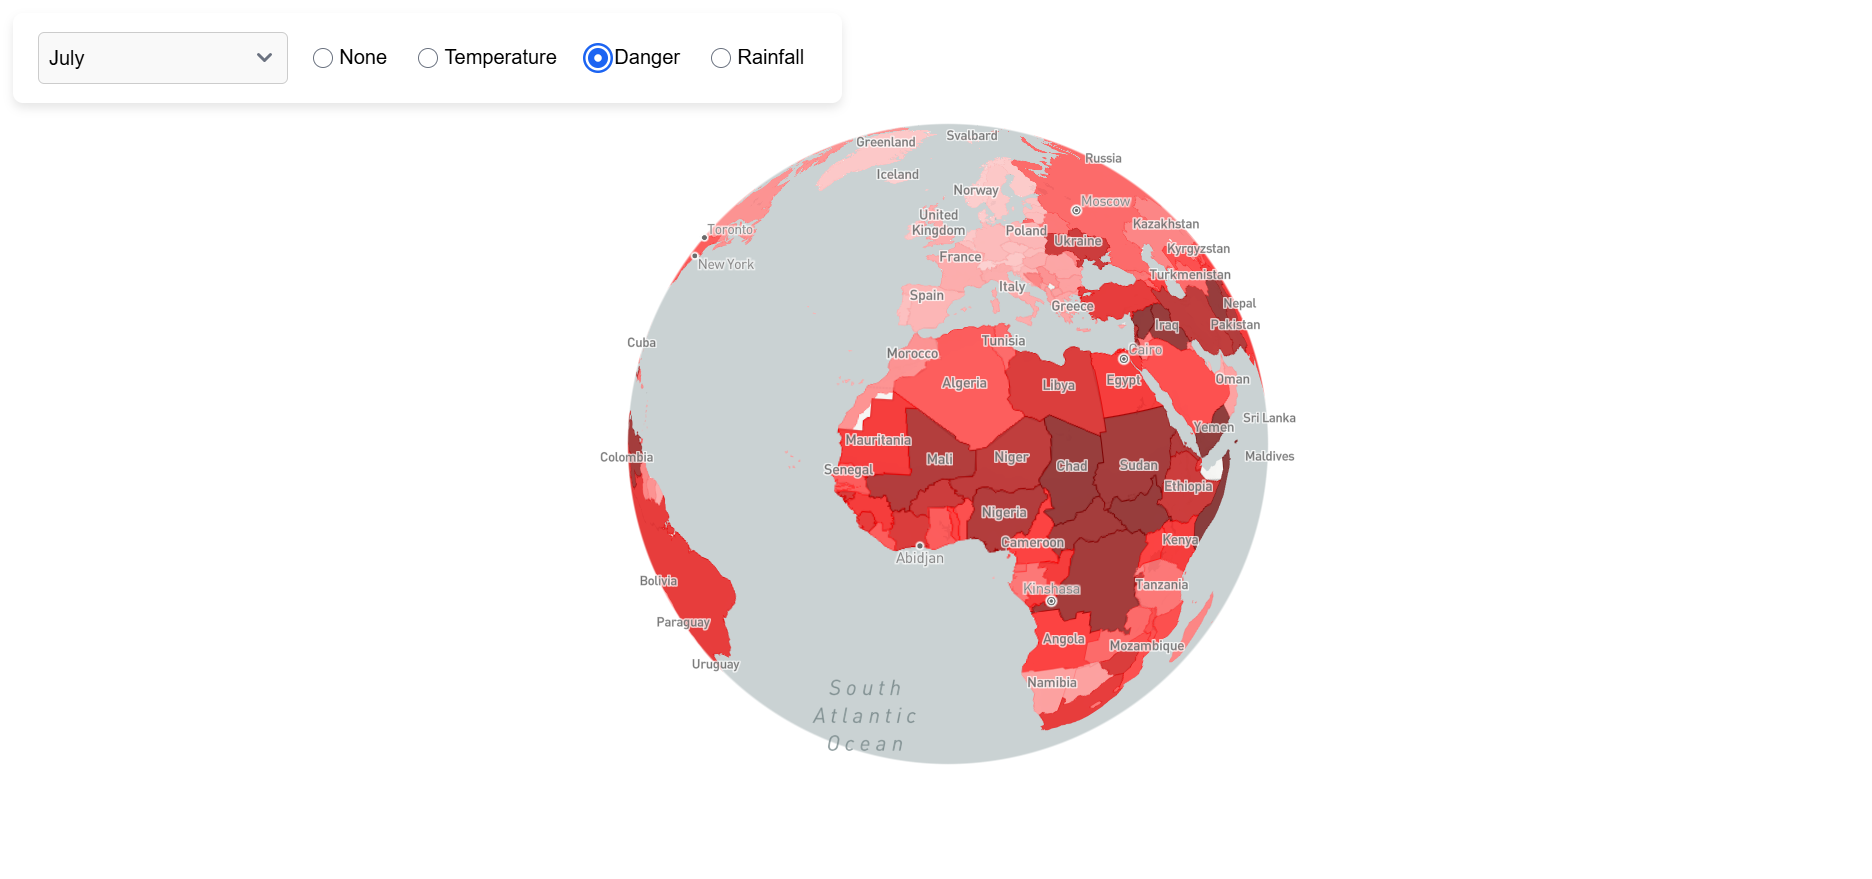
\includegraphics[width=0.4\textwidth]{6.png}
    \caption{Danger dataset visually represented in July}
    \label{fig:1}
\end{figure*}
Danger is represented in a gradient of red. This is because red has a universal association with warnings and danger, every country has its own risks and danger, a higher risk will be shown with a darker and stronger red while other countries would have a mild red. The use of red to indicate caution aligns with global conventions which makes it easier to sub consciously interpret.

\begin{figure*}[ht!]
    \centering
    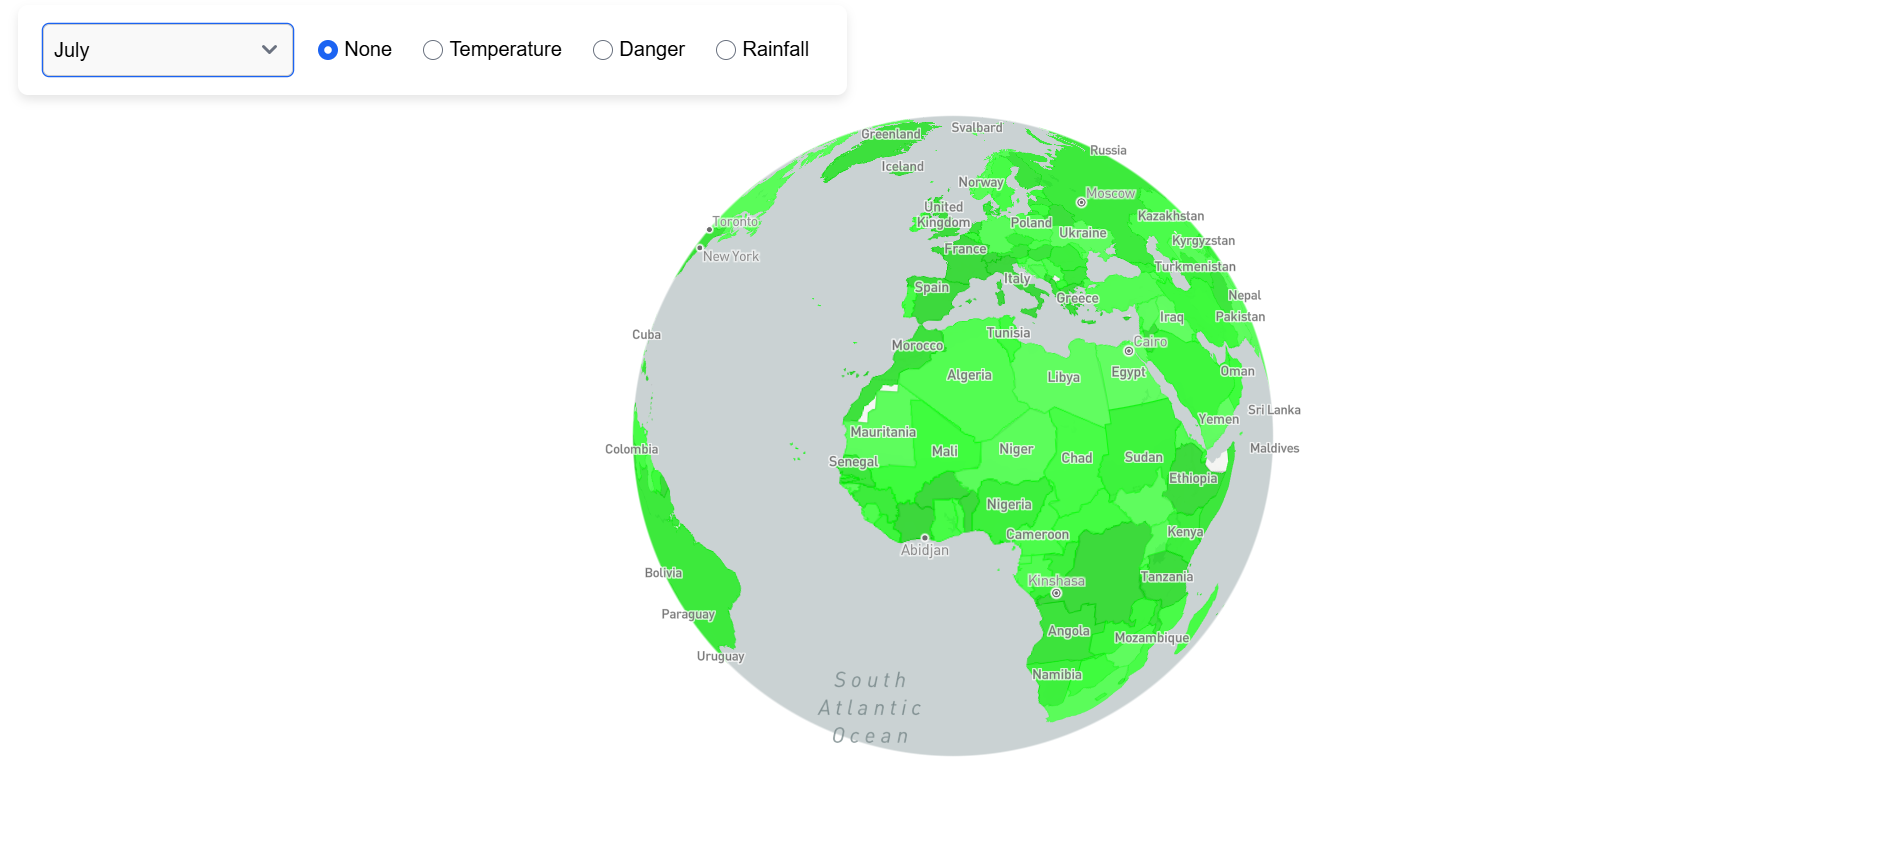
\includegraphics[width=0.4\textwidth]{7.png}
    \caption{Recommendation dataset visually represented in July}
    \label{fig:1}
\end{figure*}

\subsection{Country selection}
\subsubsection{User hovering over country}
When the user hovers over a country within the 3d travel planner the interface responds with a bold black outline around the selected country. This reinforces the users focus and provide real time feedback in the form of the country outline.

The thick black border distinguishes the country being hovered over from surrounding countries. This is effective within the interface as it provides users with immediate visual feedback to confirm their actions are registered and minimizes distractions. This follows Jakob Nielsen's usability heuristics which emphasise the need for clear feedback mechanisms.

\begin{figure*}[ht!]
    \centering
    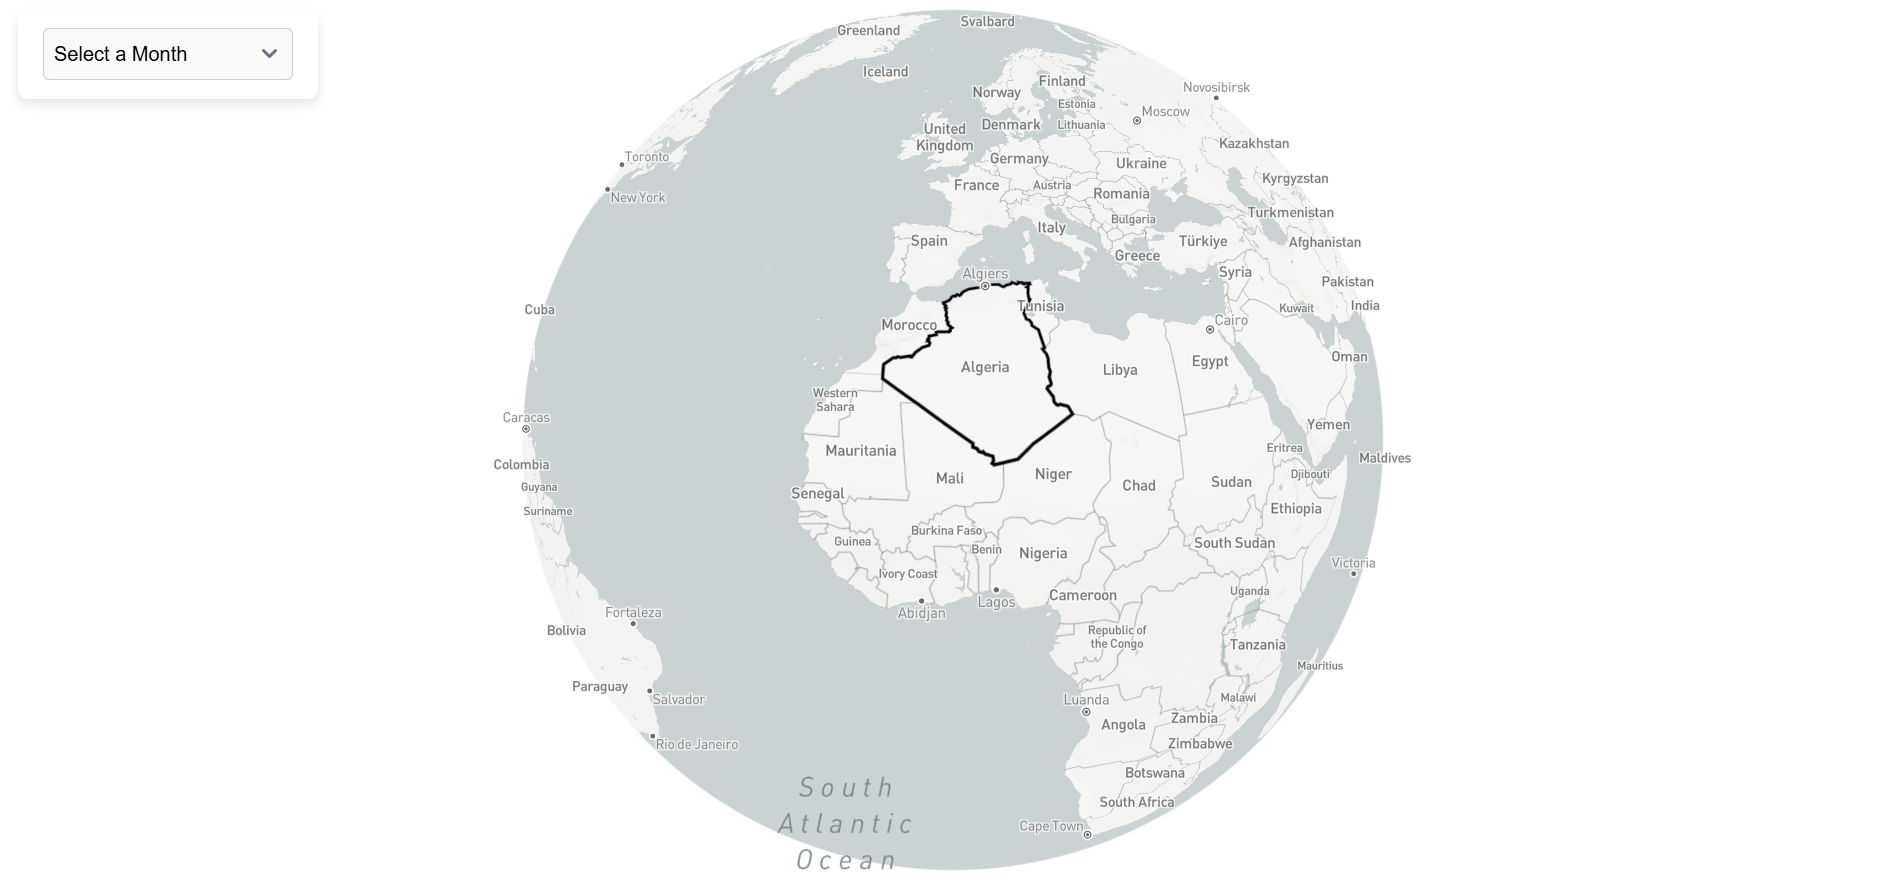
\includegraphics[width=0.4\textwidth]{8.png}
    \caption{User hovering over country response.}
    \label{fig:1}
\end{figure*}

The bold outline of the country improves scanning ability as it follows eye tracking studies completed by Faraday that show high contrast elements can reduce search time which makes navigation more efficient for the user.

\subsubsection{Country Selected By User}
When a country is selected by the user the interfaces focuses on the country and emphasising it. This is done by dimming all of the countries outside of the selected one while the chosen country remains in its original colour form, whether with a filter or not. This is a form of visual framing which is used to reduce distractions for the user and enhance their focus on the chosen country.
It aligns with the cognitive load theory presented by Sweller as it removes irrelevant information and stimuli from the interface, consequently the user is not bothered with information that it no longer useful. Bailey and Konstan suggested that removing the "visual noise" will improve the users performance. Lavie and Tractinsky found that background dimming increases attention to active zones in the interface and aids with the user flow.

\begin{figure*}[ht!]
    \centering
    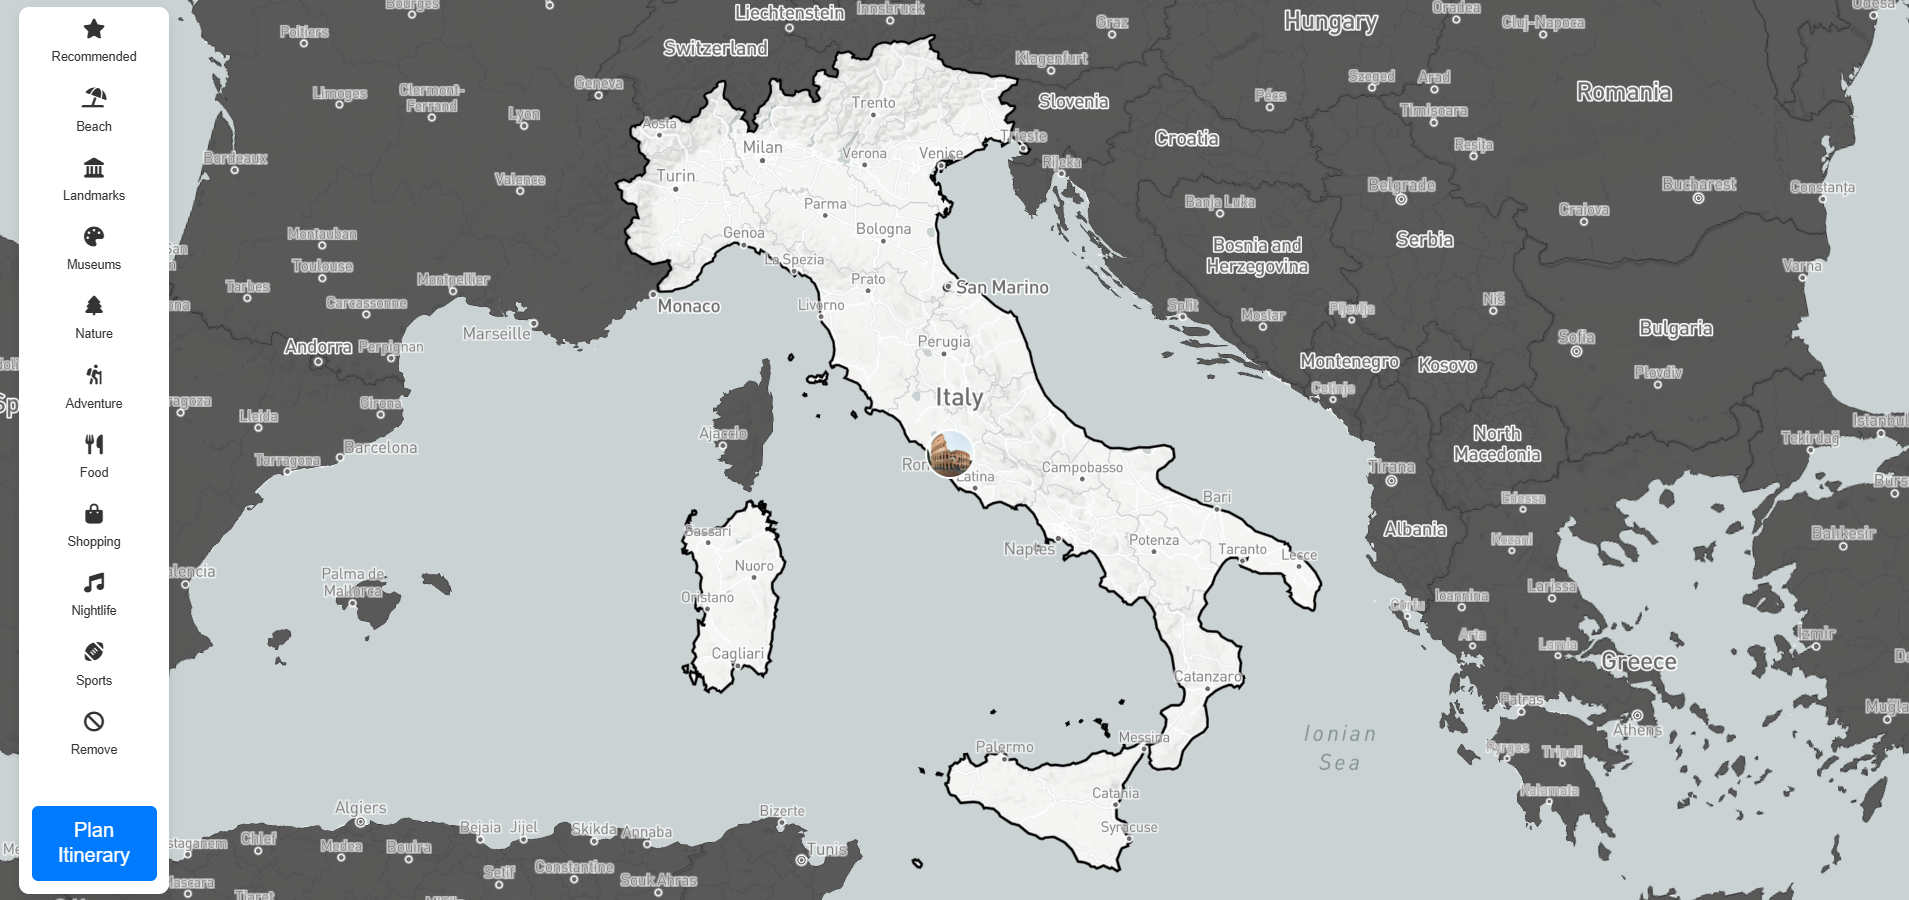
\includegraphics[width=0.4\textwidth]{9.png}
    \caption{User hovering over country response.}
    \label{fig:1}
\end{figure*}

Upon selection a vertical navigation bar appears on the left hand side of the screen which represents category filters for the map. Users are shown a clear vertical list of categorical attractions which are presented with both words and icons. This layout supports the idea of visual hierarchy by grouping related filters into a column. The column was used as Djamasbi et al confirmed that users prefer vertical scanning zones over scattered layouts on the interface.

%SHOW CLOSE UP OF THE VERTICAL FILTERS
\begin{figure*}[ht!]
    \centering
    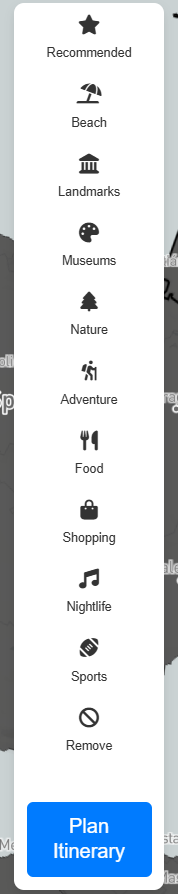
\includegraphics[height=0.4\textwidth]{Vertical filters.png}
    \caption{User hovering over country response.}
    \label{fig:1}
\end{figure*}

Further more the use of icons reduce cognitive effort and make the filters understandable and accessible to a vast variety of users as well as navigating around a language barrier. This is because icons are universally recognisable. Accessibility is also achieved as the black text on a white background achieves WCAG recommended contrast ratio which will help with readability for users with low vision.

\newpage

MARKERS:
An important feature at this point in the interface is the dynamic zoom based marker system. It has been created to reveal information incrementally to the user as they explore the country. Initially only the most popular and relevant attractions or points of interest are visible on the map, however as the user zooms further into the country more attractions and points of interest will appear.

%SHOW MARKERS IN INITAL STATE
\begin{figure*}[ht!]
    \centering
    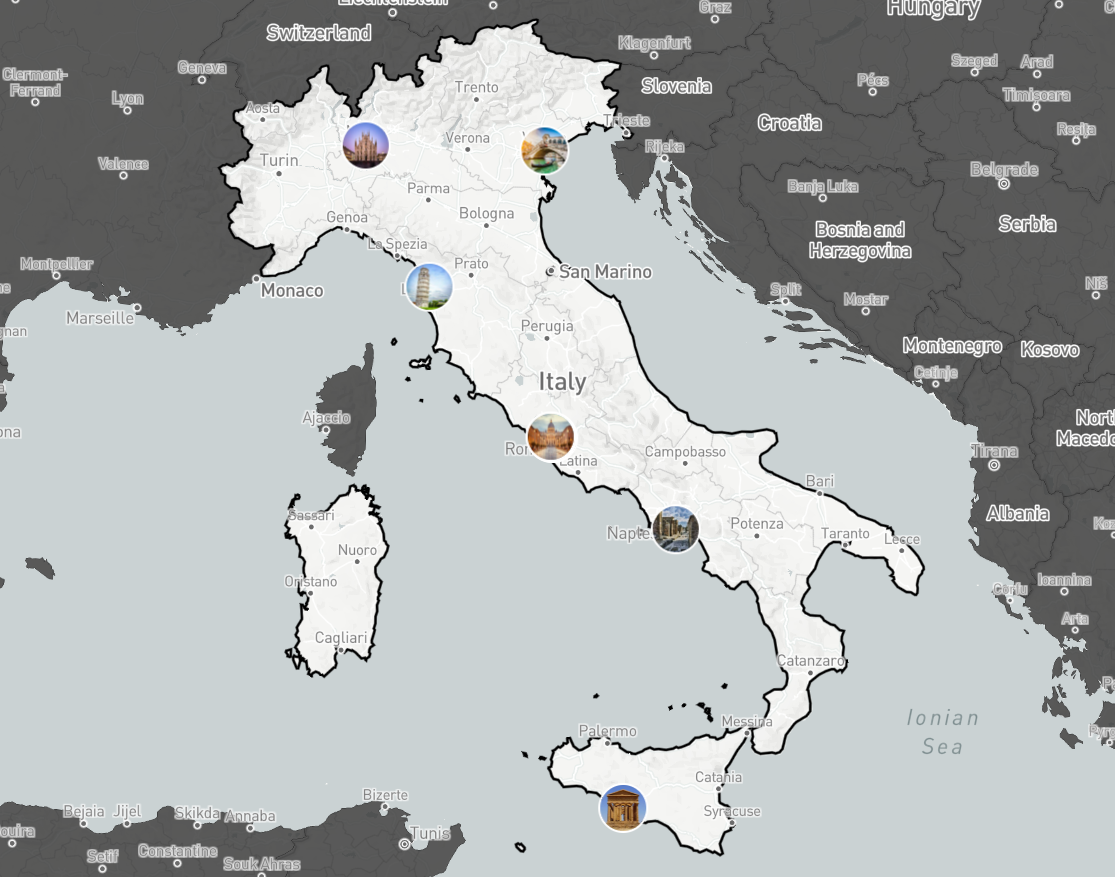
\includegraphics[width=0.4\textwidth]{basezoom.png}
    \caption{Baseline zoom when the user is loaded in}
    \label{fig:1}
\end{figure*}
%SHOW MARKERS IN ZOOMED STATE
\begin{figure*}[ht!]
    \centering
    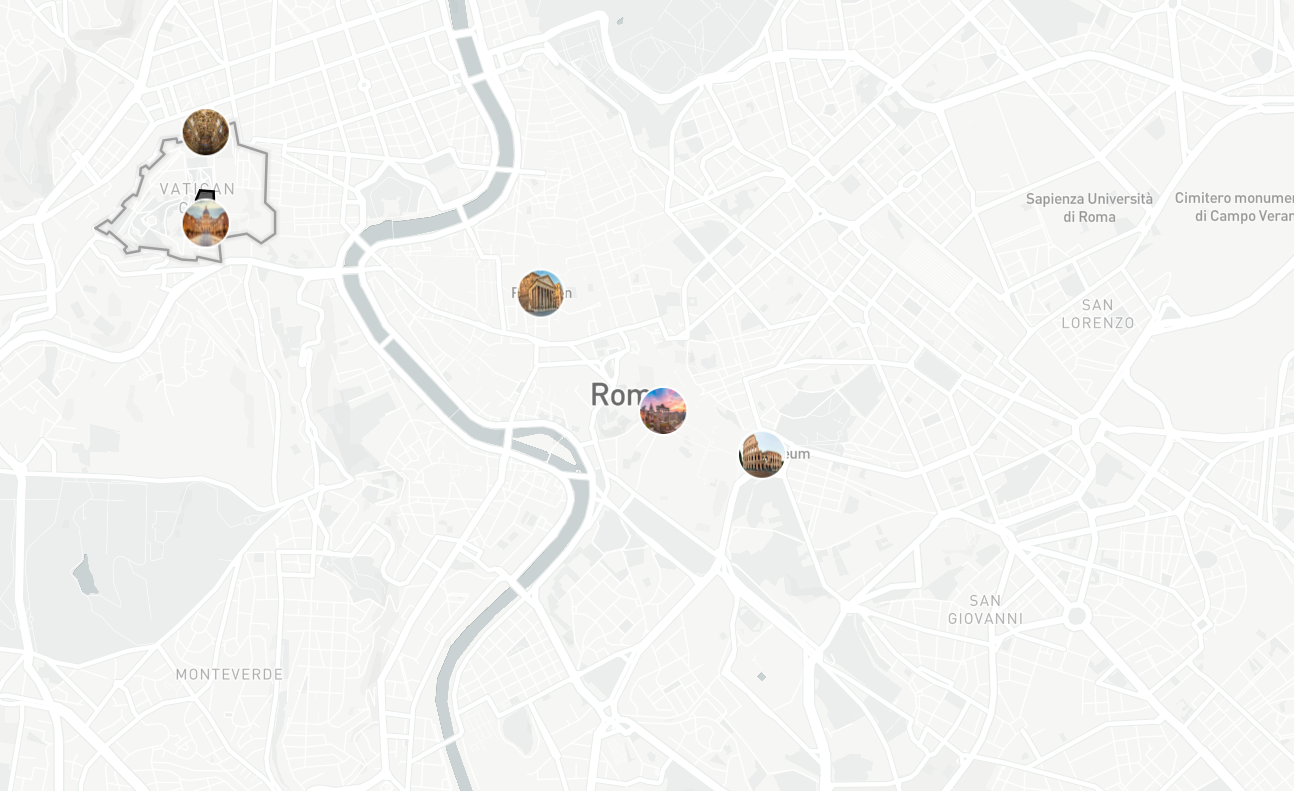
\includegraphics[width=0.4\textwidth]{biggerzoom.png}
    \caption{User has zoomed into Rome to view more attractions}
    \label{fig:1}
\end{figure*}

Progressive Disclosure through Zoom Levels:
At the initial zoom level the user will be presented with Key national landmarks.

%SHOW FIRST ZOOM STATE

As the user zooms in further they will be presented with secondary points of interests that are popular.

%NEXT ZOOM STATE
\begin{figure*}[H]
    \centering
    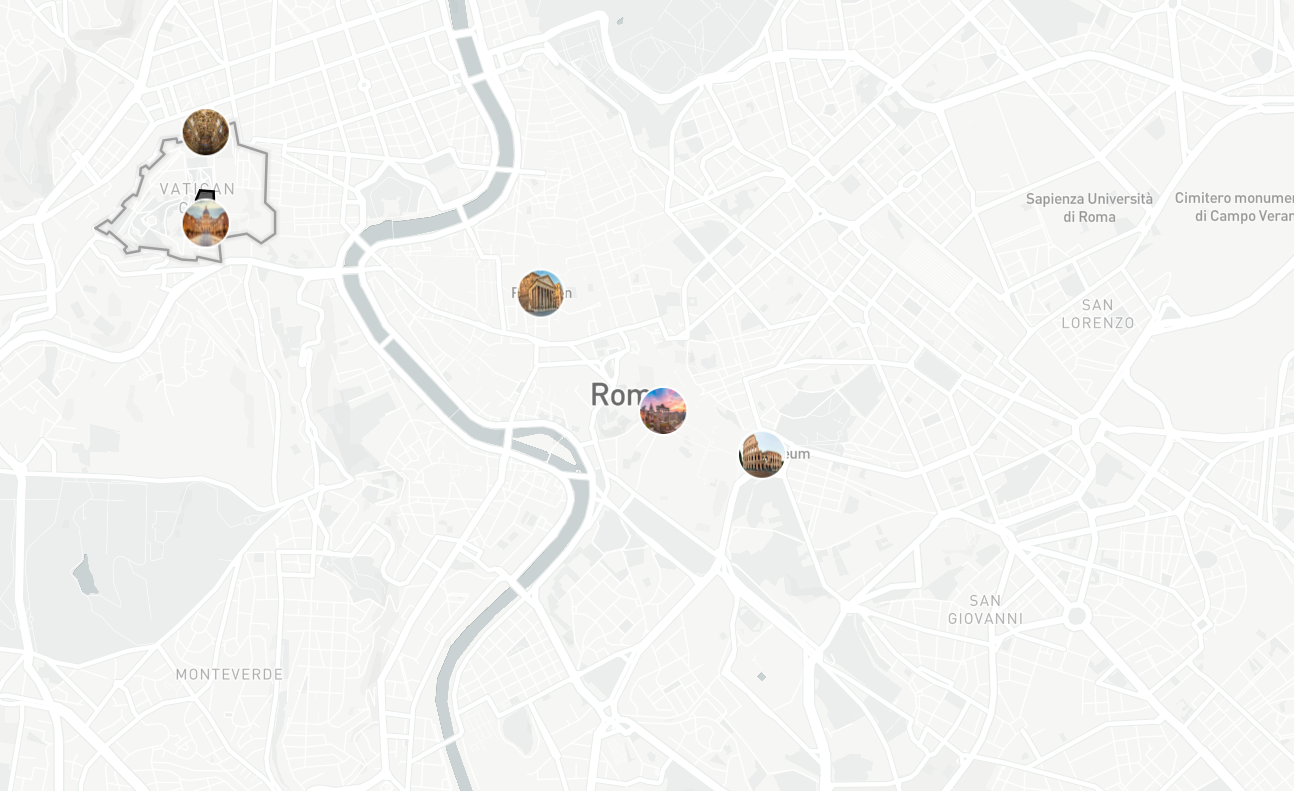
\includegraphics[width=0.4\textwidth]{biggerzoom.png}
    \caption{User has zoomed into Rome to view more attractions}
    \label{fig:1}
\end{figure*}

Zoom based filtering is an implementation of progressive disclosure which was found by Nielsen and supported by research from Bailey and Konstan who found that interfaces that reveal data in stages have up to a 26 percent higher usability rating and lower cognitive load on the user.

Furthermore the interface follows a visual hierarchy and guides the users attention logically by spacing the marker density over multiple zoom stages. This allows the user to only focus on the relevant markers at each zoom and makes sure that they are presented cleanly.

\subsubsection{Plan Itinerary Selected}

When the user selects the "Plan Itinerary" button from the vertical menu a modal window will appear on the screen grabbing the users attention.
The modal separates the attractions and visiting options into defined tabs at the top of the screen. The tab at the top of the screen supports flat information architecture which in this case reduced the number of clicks the user will need to find their desired information. The tab the is highlighted in blue directs the users attention to that category.

%SHOW THE MODEL POP UP
\begin{figure*}[H]
    \centering
    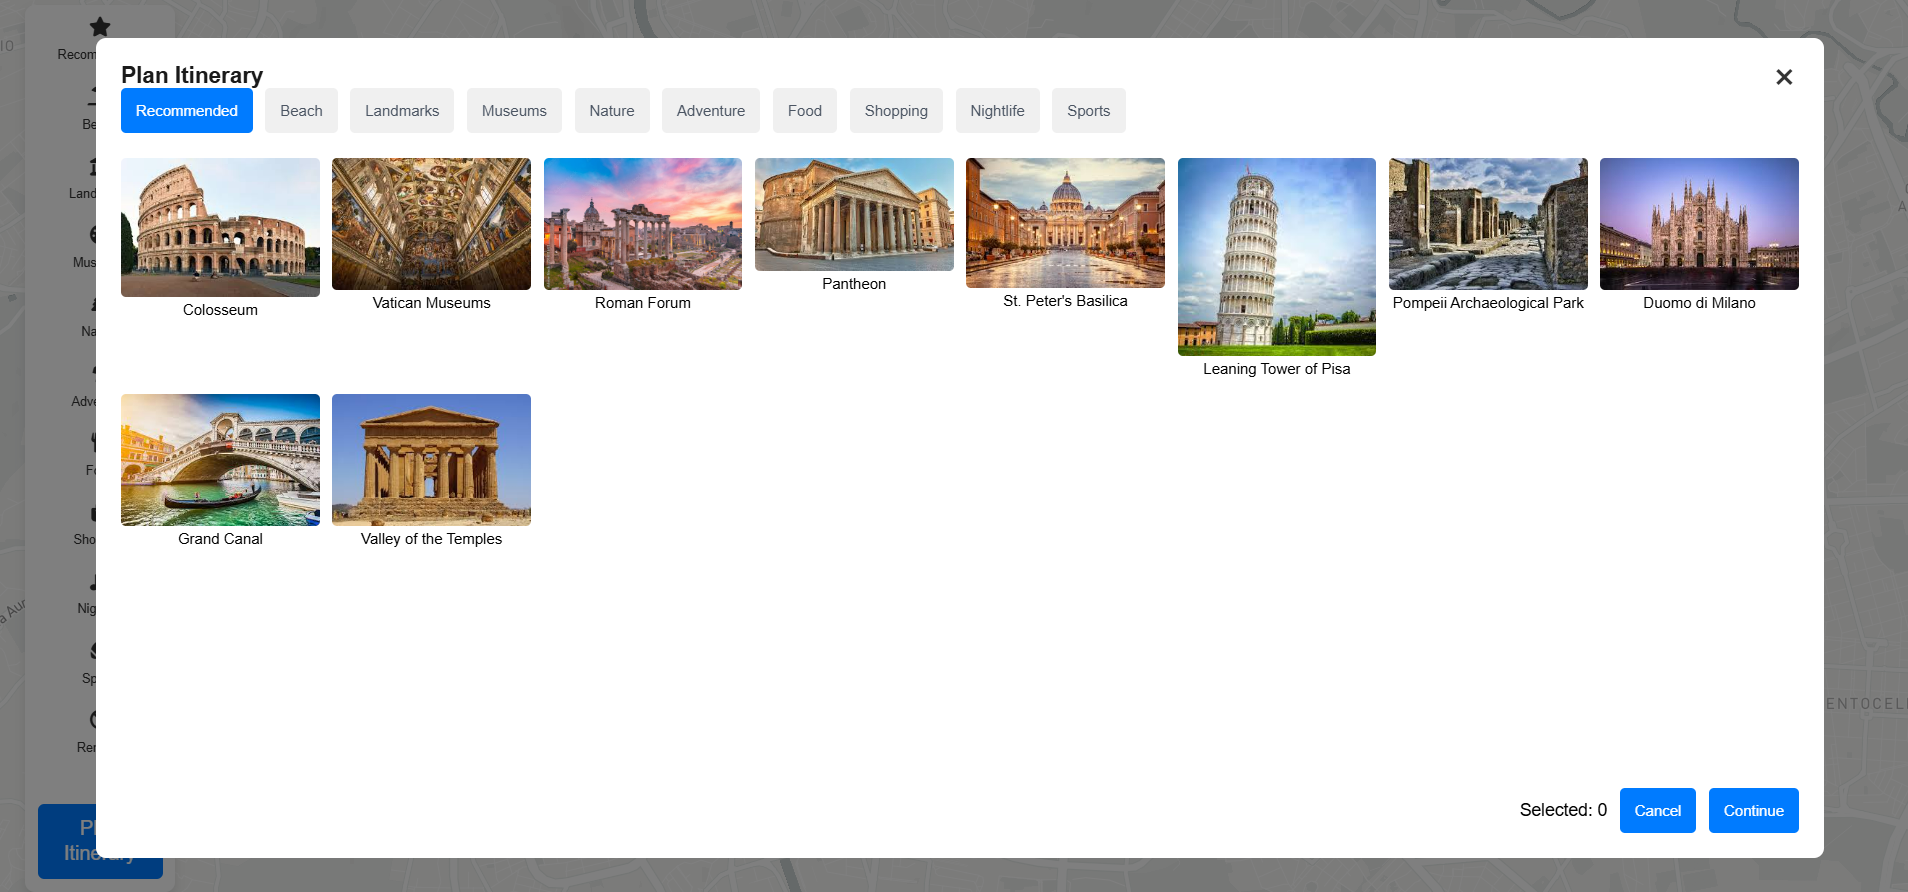
\includegraphics[width=0.4\textwidth]{planItin.png}
    \caption{User has zoomed into Rome to view more attractions}
    \label{fig:1}
\end{figure*}

The content is presented as large image cards which have pictures of the attraction or activity as well as a caption.

The modal implements progressive disclosure by avoiding presenting all of the possible activities and attractions at once. This helps avoid decision fatigue and simplifies visual scanning. This is because Djamasbi et al showed that well grouped content on interfaces enables faster comprehension.

%SHOW THE TABS
\begin{figure*}[ht!]
    \centering
    
\includegraphics[width=0.4\textwidth]{tabs.png}
    \caption{User has zoomed into Rome to view more attractions}
    \label{fig:1}
\end{figure*}

Furthermore the modal has a selection tracker implemented at the bottom right which provides users with immediate feedback on their actions when it comes to selecting activities or places of interest. This supports Nielsen's usability heuristics around the visibility of system status to the user.

%SHOW IMAGE OF THE ACTIVITY COUNTER IN THE BOTTOM RIGHT
\begin{figure*}[ht!]
    \centering
    \begin{minipage}[t]{0.4\textwidth}
        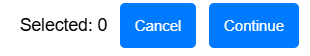
\includegraphics[width=\textwidth]{0 selected.png}
    \end{minipage}
    \hfill
    \begin{minipage}[t]{0.4\textwidth}
        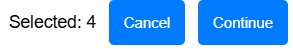
\includegraphics[width=\textwidth]{4 selected.png}
    \end{minipage}
    \caption{Example of good layouts to showcase artists}
    \label{fig:1}
\end{figure*}

Cancel and continue buttons are placed to follows Fitts law and conventional web behaviour as the user will be used to that. This makes the interface more intuitive to use.

These buttons and tiles for selection of activities have rounded corners and hover effects to make the interface seem more friendly and engaging to the users, this gives them comfort to explore. These small details increases the perceived usability and trust as stated by Googles user experience research.

%SHOW IMAGE OF THE PLAN ITINERARY SCREEN LOADING
\begin{figure*}[ht!]
    \centering
    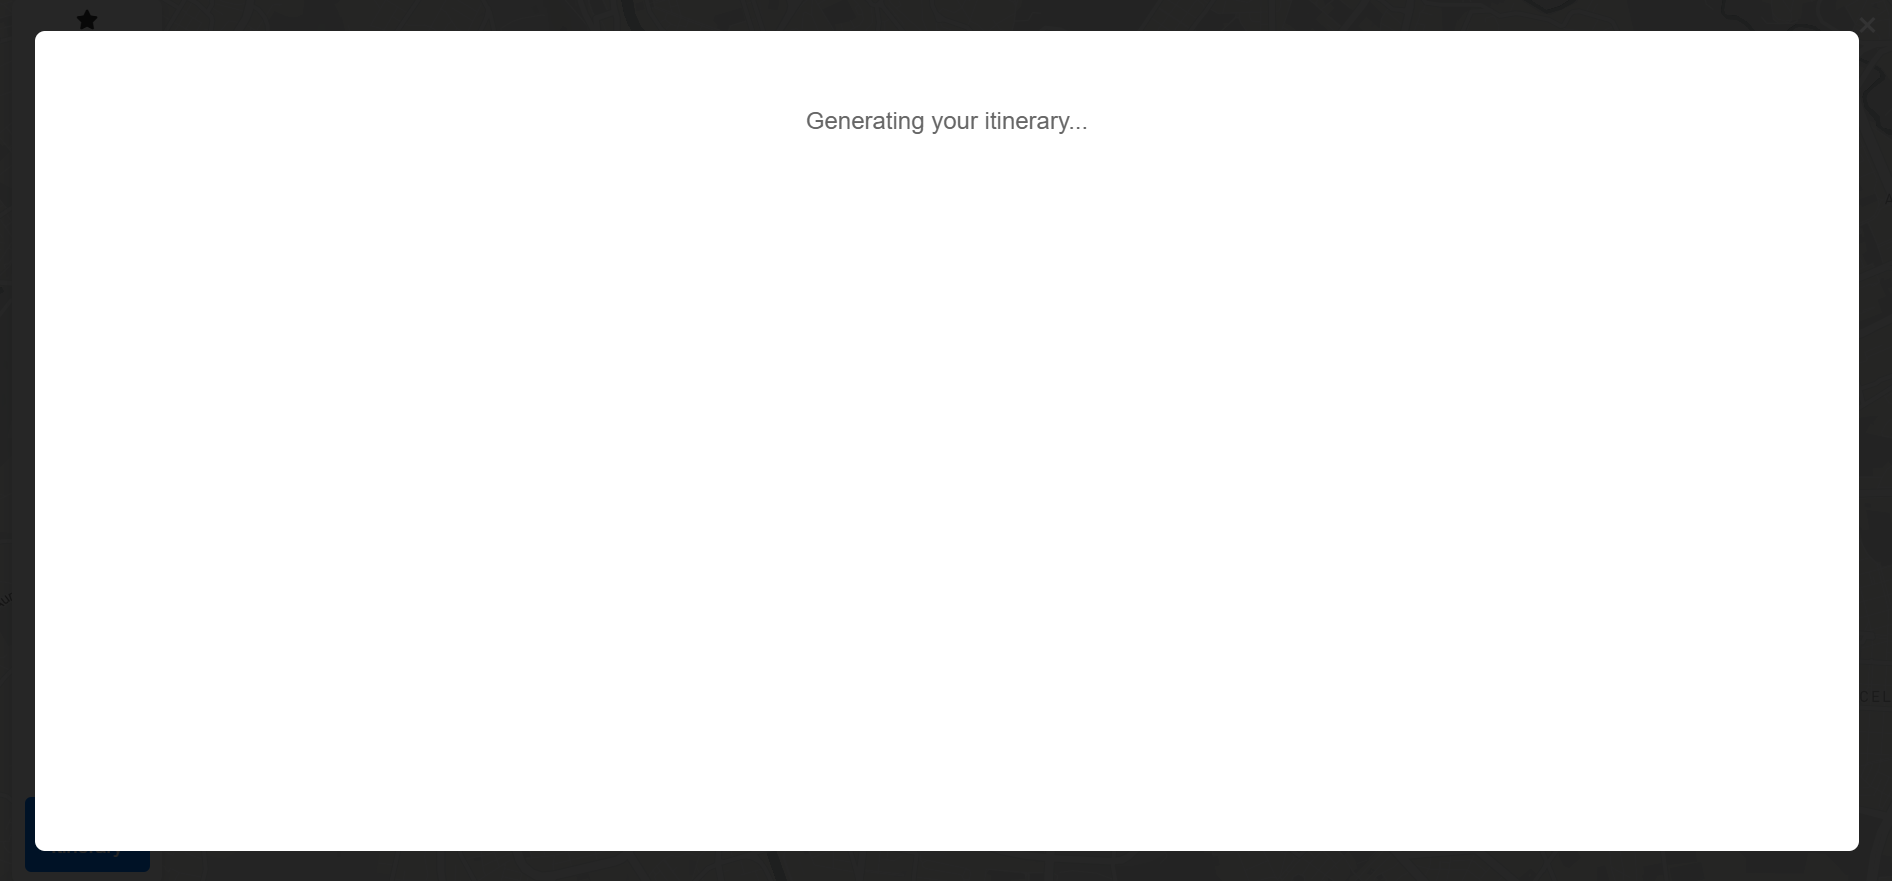
\includegraphics[width=0.4\textwidth]{loading screen.png}
    \caption{User has zoomed into Rome to view more attractions}
    \label{fig:1}
\end{figure*}

%SHOW IMAGE OF THE ITINERARY PLAN
When the itinerary is generated a timeline is presented that improves the user comprehension by 32 percent due to the linear and sequential mapping.

Cards are used to enforce the chunking principle of information, also putting all similar information together.


\begin{figure*}[ht!]
    \centering
    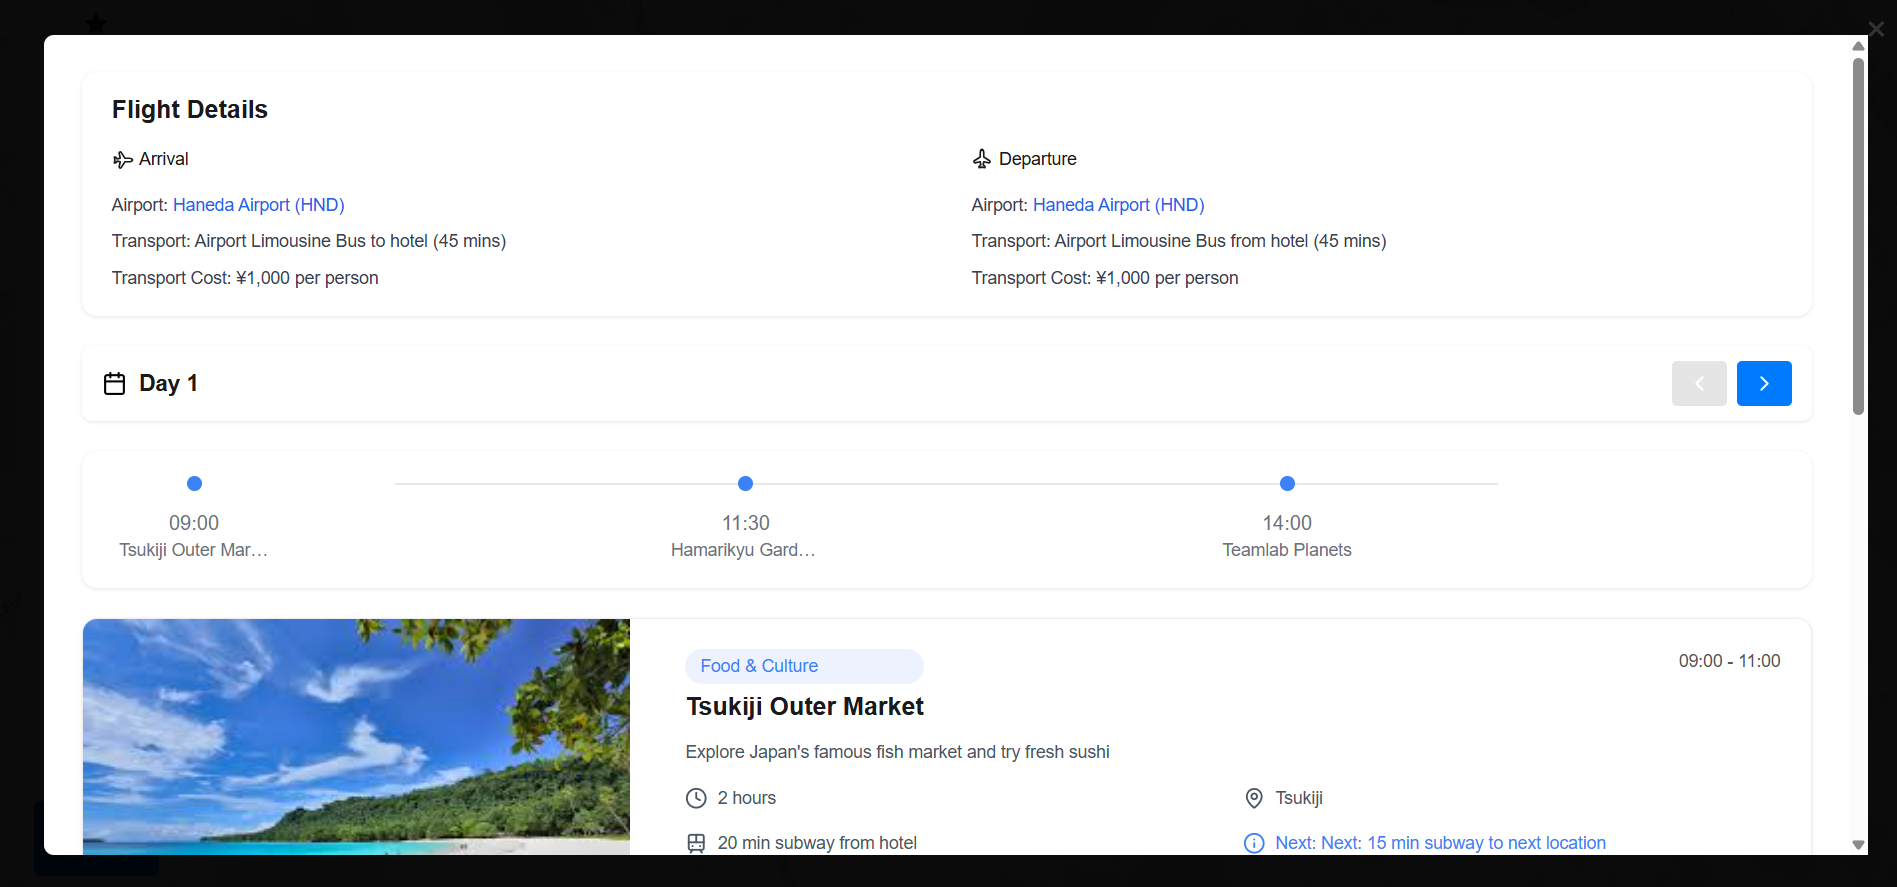
\includegraphics[width=0.4\textwidth]{itin1.png}
    \caption{User has zoomed into Rome to view more attractions}
    \label{fig:1}
\end{figure*}

The page categorises the activities such as "Food and culture" or "nature" and improves user recognition by 36 percent according to Rosch research which calls this "categorical perception".

The page includes day based navigation with bi directional control of days meaning that the user can navigate forwards and backwards through days and through the itinerary.
By consistently using this layout errors are reduced by 31 percent as it has navigational consistency and follows Card et als research.

\begin{figure*}[ht!]
    \centering
    \begin{minipage}[t]{0.4\textwidth}
        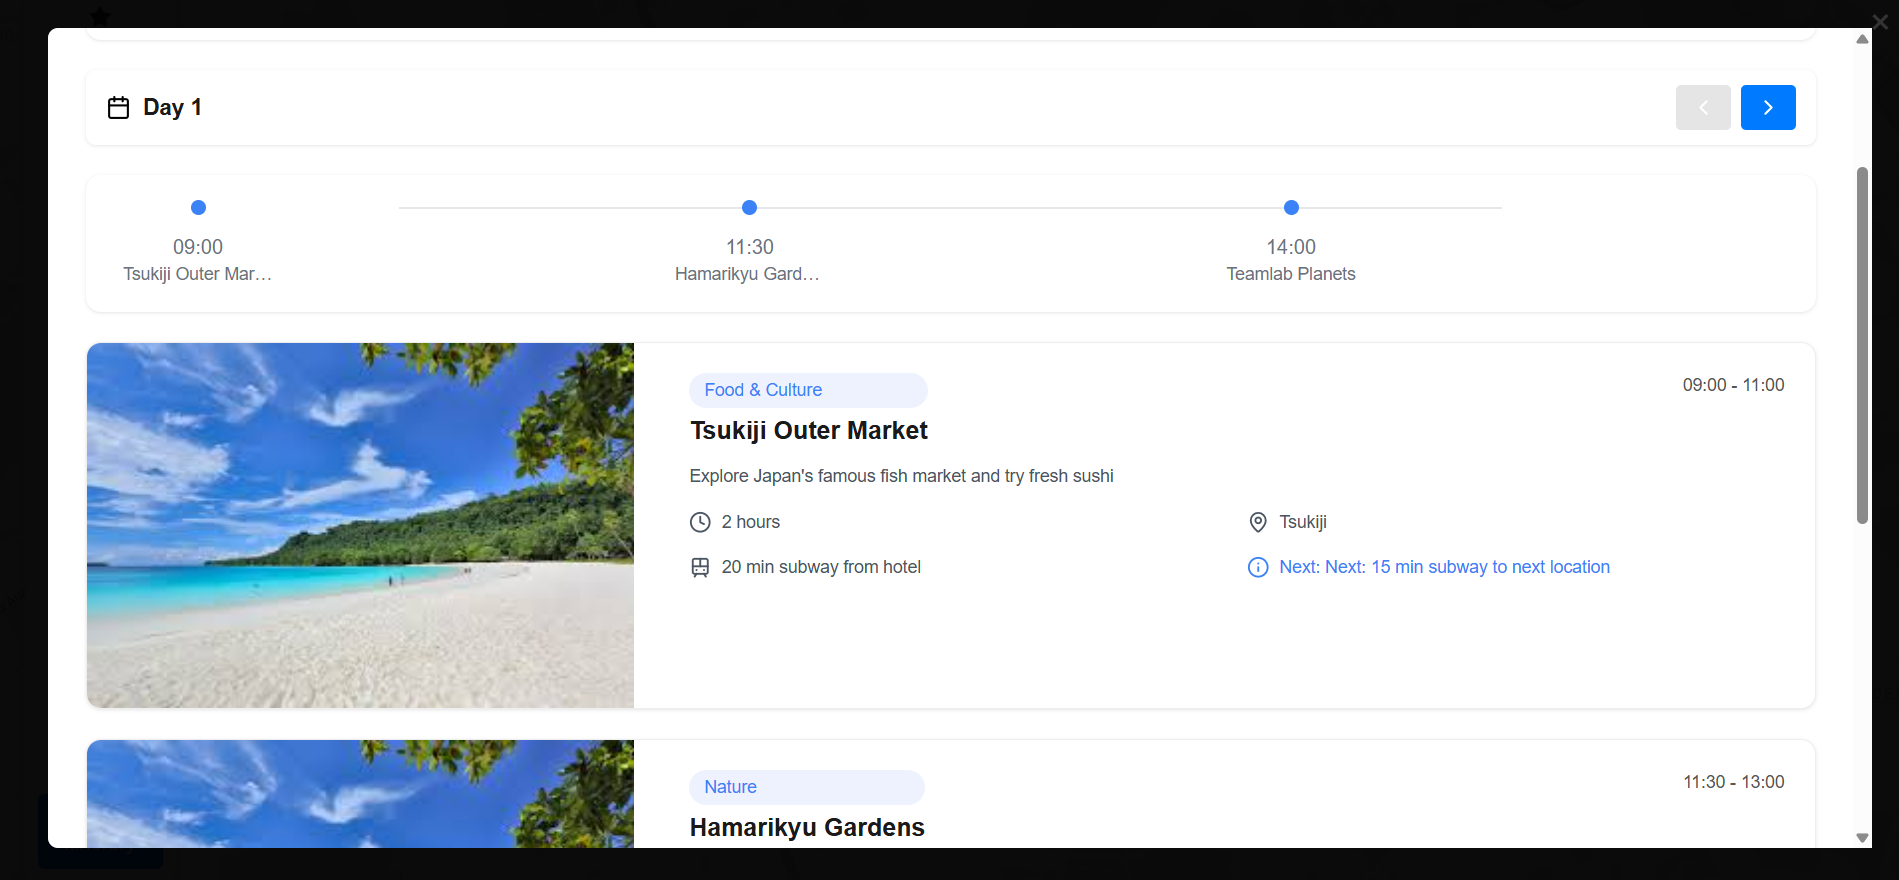
\includegraphics[width=0.4\textwidth]{itin2.png}
    \end{minipage}
    \hfill
    \begin{minipage}[t]{0.4\textwidth}
        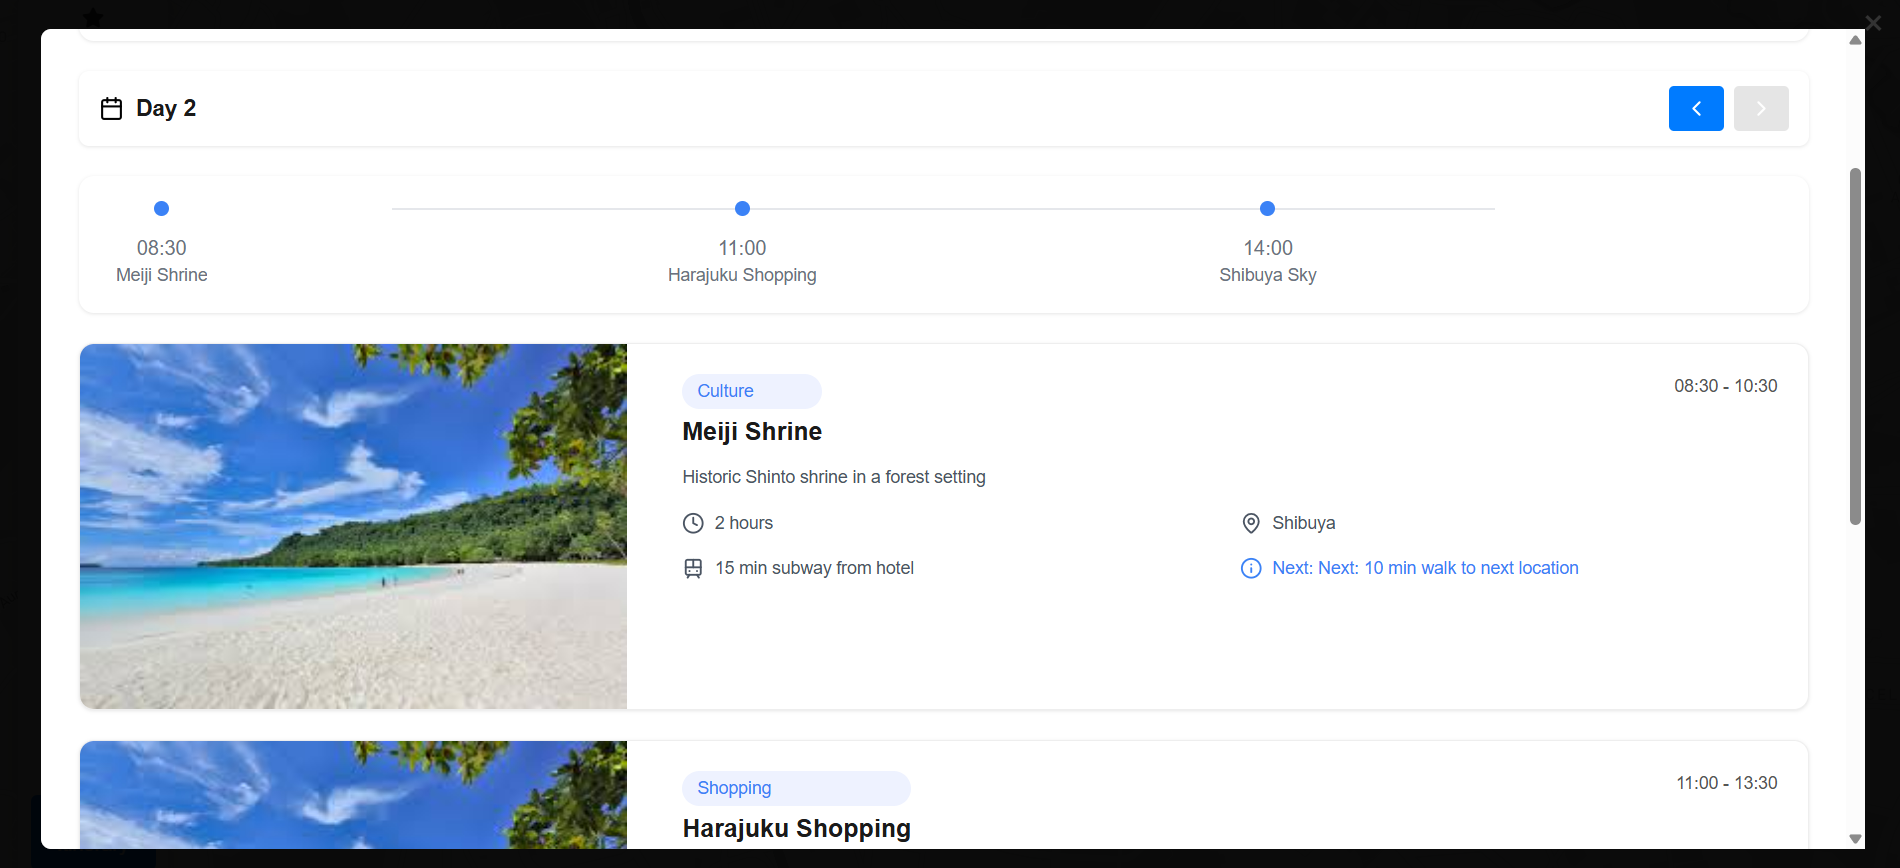
\includegraphics[width=0.4\textwidth]{itin3.png}
    \end{minipage}
    \caption{Example of good layouts to showcase artists}
    \label{fig:1}
\end{figure*}


\newpage




\section{Mobile Recipe App}
The Mobile Recipe App is a Cooking App that prioritises accessibility and ease of use for the elderly and visually impaired users. It does this by reducing cognitive load and enhancing the user experience through human computer interaction principles such as consistency, and implements research from interactions with computers to how differently abled user would see the screen to cater every element from the colour schemes to the typography for the users. This means that standards such as WCAG AAA have been met and ensure that the app is inclusive and easy to use.

\subsection{Welcome Screen}
The Welcome Screen is the first interaction for the user and is an entry point to the app which provides clear options to the user that include Log In, Sign Up and Continue as a Guest.

The global population of over 65 sis projected to double by 2050 according to the world health organisation with 80 percent experiencing a vision decline. As well as 285 million people in the world who live with visual impairments led me to create a specific starting colour scheme.

The navy blue background with white text (14:1 contrast ratio) substantially exceeds WCAG AAA requirements. Owsley's longitudinal studies (2001, 2011) demonstrated that contrast sensitivity declines approximately 25 percent per decade after age 65, requiring higher contrast for equivalent visibility.

For the guest button I selected yellow (FFD700) based on Okabe and Ito's research establishing a universal design colour palette. Their work at Tokyo University demonstrated this specific yellow remains distinguishable across all three major types of colour blindness—protanopia, deuteranopia, and tritanopia—affecting 8 percent of males and 0.5 percent of females.

%HERE ADD AN IMAGE SHOWING THE COLOUR PALETTE
\newpage

\begin{figure*}[ht!]
    \centering
    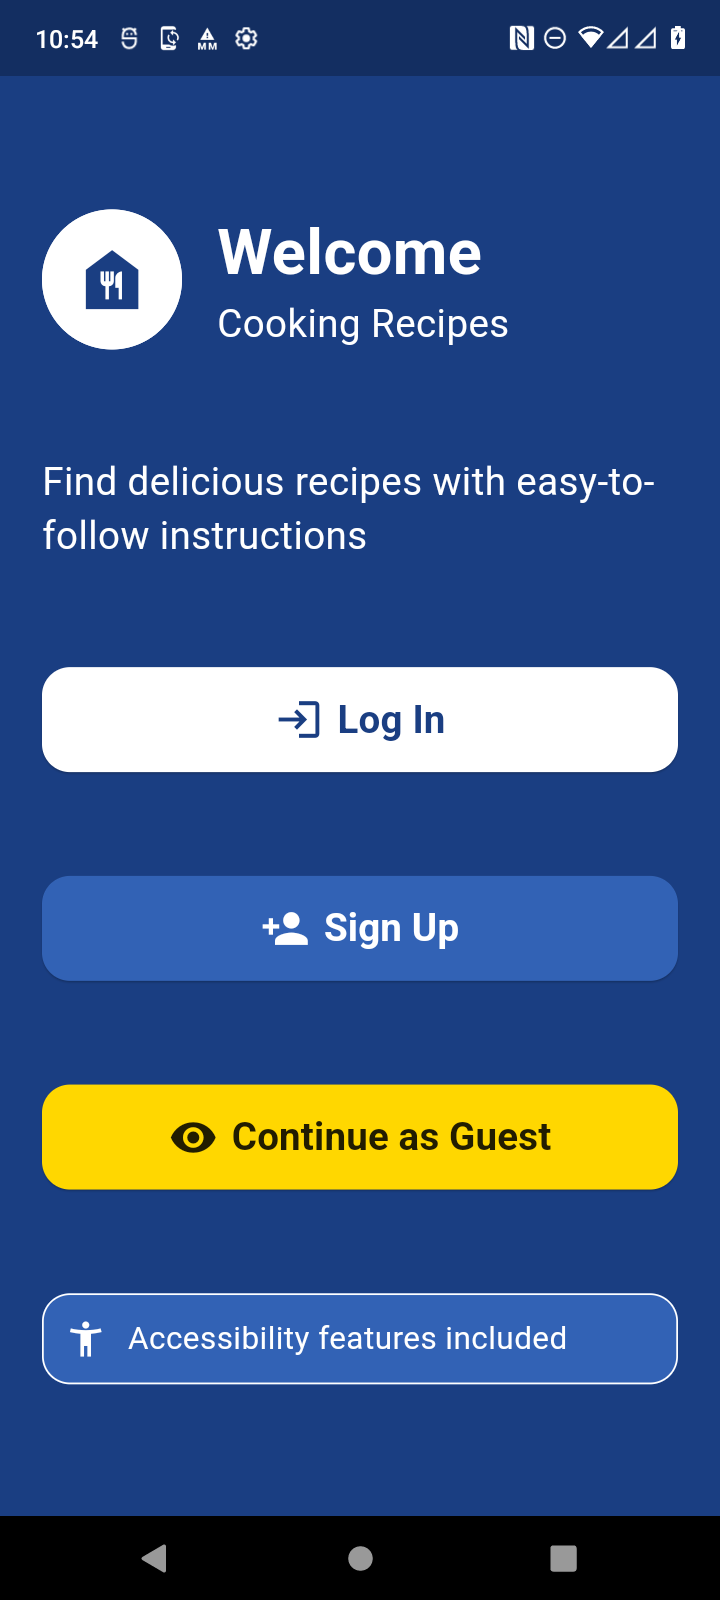
\includegraphics[height=0.4\textwidth]{10.png}
    \caption{Welcome Screen}
    \label{fig:1}
\end{figure*}

Button shapes incorporate Nielsen Norman Group findings showing rounded corners reduce cognitive processing time by 9 percent for elderly users. Also sharp corners create additional fixation points that require extra cognitive processing which is not needed for our targeted users and can become problematic with age related working memory decline.

MIT Age Lab's touch studies (Jin et al., 2007) established that users over 65 experience a 26 percent higher touch error rate than younger adults. This meant that they provided a recommendation from their research which was for there to be a minimum 16.5mm touch target, based on this I made the button design full width across the screen which gives the user a large touch target even with reduced motor precision.

%HERE ADD IMAGE SHOWING BUTTONS, SIZE AND EDGES
\begin{figure*}[ht!]
    \centering
    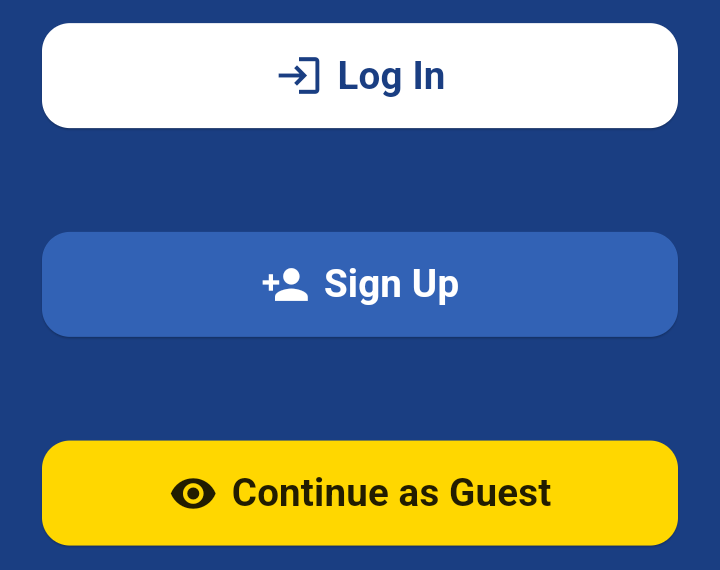
\includegraphics[width=0.5\textwidth]{m1.png}
    \caption{Size of buttons and curved edges}
    \label{fig:1}
\end{figure*}


Stanford completed a study in the visual aging laboratory on scan path efficiency. Their eye tracking studies showed that AMD patients showed vertical scanning preserves 80 percent efficiency in comparison to 47 percent efficiency for horizontal patterns. This aided me to make the decision to stack the buttons one on top of the other vertically.

Gestalts principles of perceptual organisation  are followed with this button ordering in my welcome page as it creates a natural progression that Hawthorns research showed as reducing cognitive load for users with early stage dementia. This is also a demographic that comes with elderly.

%SHOW HOW THE BUTTONS ON THE WELCOME SCREEN ARE STACKED

I decided to use text and icons throughout the page which is supported by Paivios Dual Coding Theory which shows that cognitive processing and memory retention increase when the user is shown both verbal and visual cues, in this case, text and icons representing the same button or information.

%SHOW THE ICONS AND TEXT ON THE BUTTONS

\subsection{Login Screen}
The login screen is a entry point to the cooking app and allows the user to enter by inputting their credentials to be verified, in this case an username and password. It also includes options like “Remember Me” for convenience, “Forgot Password?” for recovering lost credentials, and demo credentials for users who wish for quick access to the account features.

The Navy header with a 14:1 contrast ratio continues from the welcome screen which provides consistency for the user and is a key principle in human computer interaction.
Further more the Yellow sign in button also keep consistency with the welcome screens colour hierarchy and gives the user the maximum clarity and visibility due to the 16:1 contrast with black text, this will help all users including ones that have achromatopsia, which is complete colour blindness.

The Yellow Sign In bar has been used as a visual cue and driver in the page that draws the users attention away from the colour scheme as a call to action.

Continues with consistency of resarch shown before with the rounded corners and hierarchy and button sizes.

%SHOW THE SIGN IN SCREEN, FOCUS ON THE COLOURS AND YELLOW BUTTON
\begin{figure*}[ht!]
    \centering
    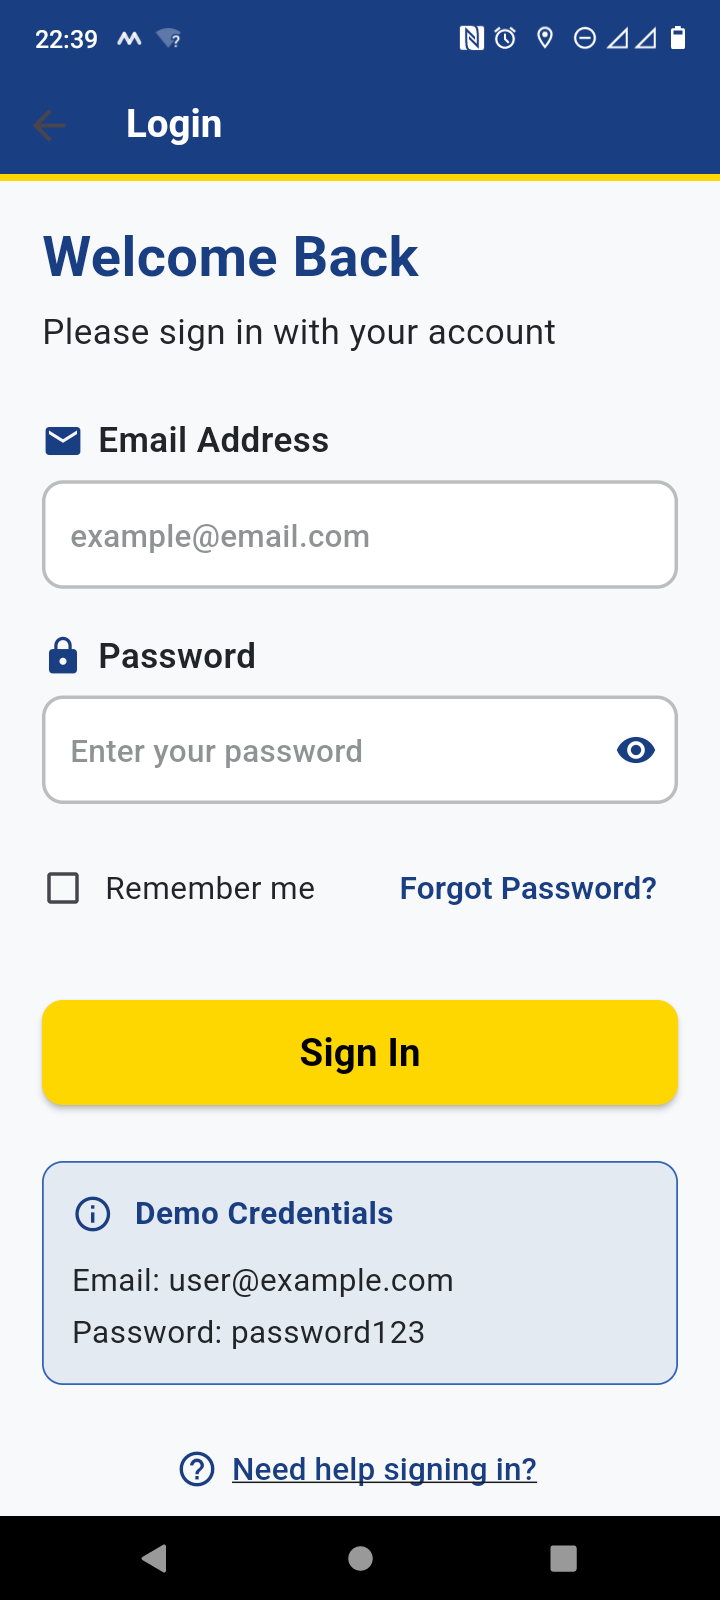
\includegraphics[height=0.4\textwidth]{M Login screen.png}
    \caption{Size of buttons and curved edges}
    \label{fig:1}
\end{figure*}

Light grey background has been used to provided a subtle contrast against the white (3:1 ratio) without creating visual strain as there have been studies completed by Wolffsohn et al of glare sensitivity to elderly users.

Sayago and Blat found that 78 percent of elderly users struggle with password entry and prefer visible confirmation, this lead to my implementation of the password visibility toggle.
\newpage
%SHOW THE SIGN IN VISIBILIY PASSWROD TOGGLE
\begin{figure*}[ht!]
    \centering
    \begin{minipage}[t]{0.4\textwidth}
        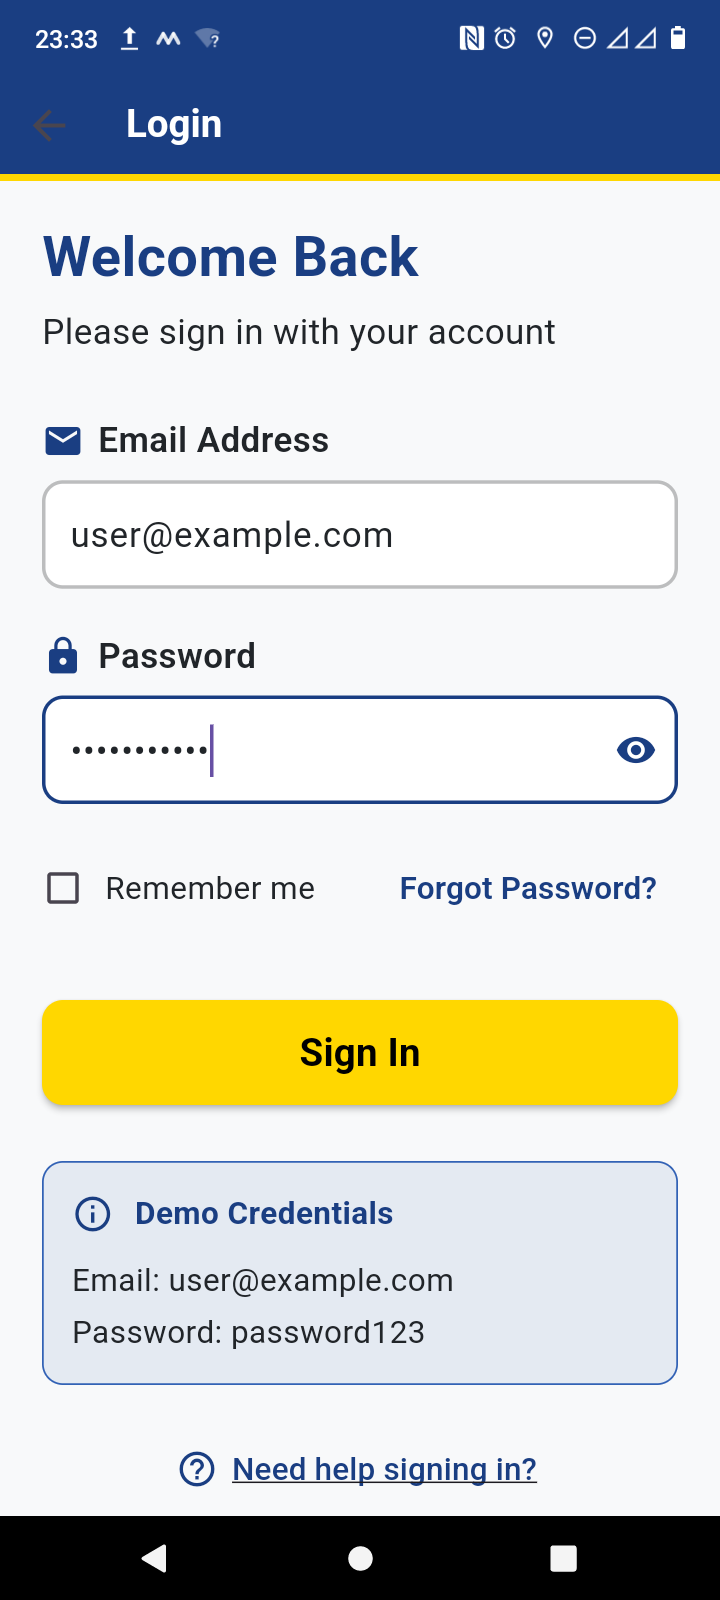
\includegraphics[height=\textwidth]{M hidden pass.png}
    \end{minipage}
    \hfill
    \begin{minipage}[t]{0.4\textwidth}
        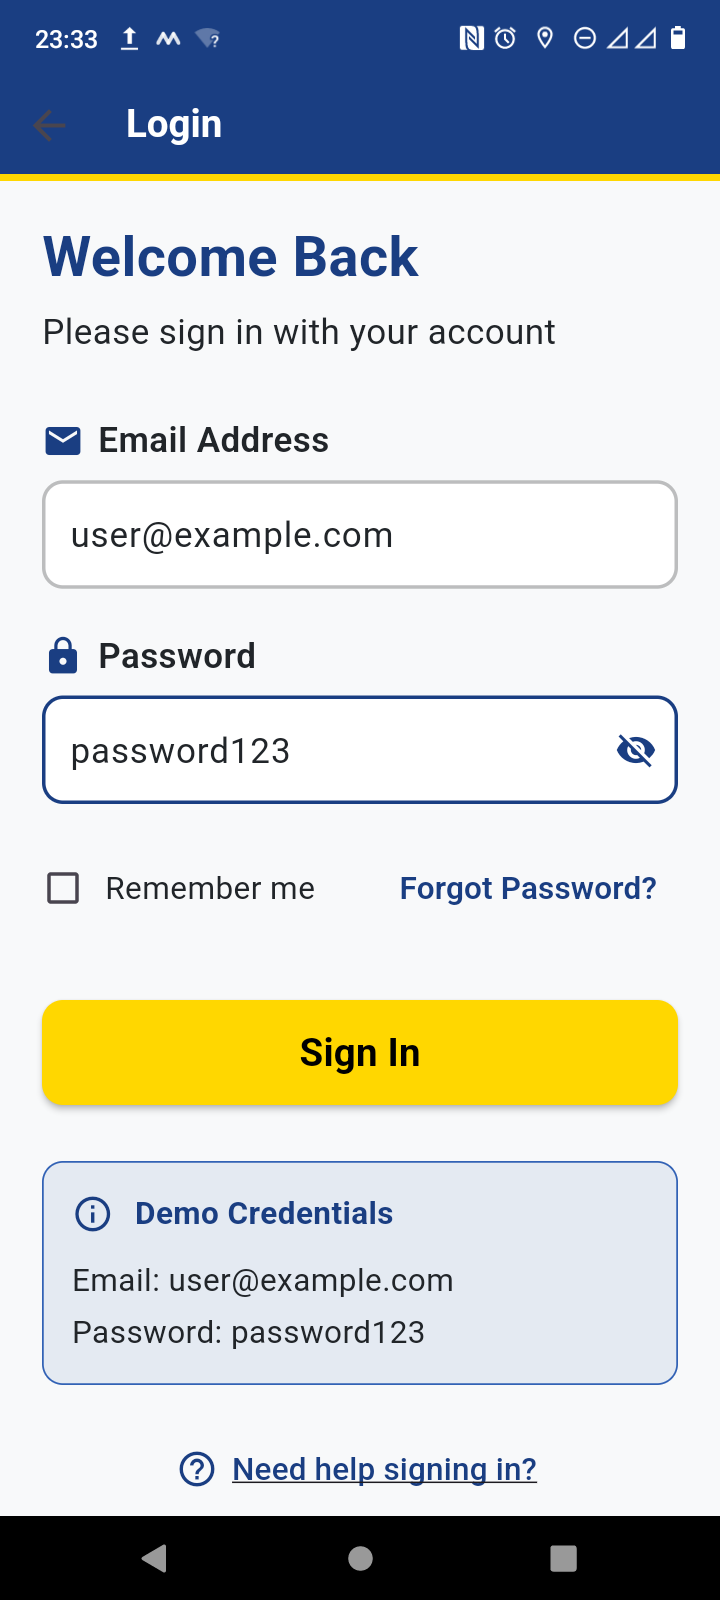
\includegraphics[height=\textwidth]{M shown pass.png}
    \end{minipage}
    \caption{Example of good layouts to showcase artists}
    \label{fig:1}
\end{figure*}

The Demo credentials box uses Nielsen's recognition-over-recall principle, which reduces cognitive load to the user by providing working login details.

%SHOW THE DEMO CREDENTIALS PICTURE
\begin{figure*}[ht!]
    \centering
    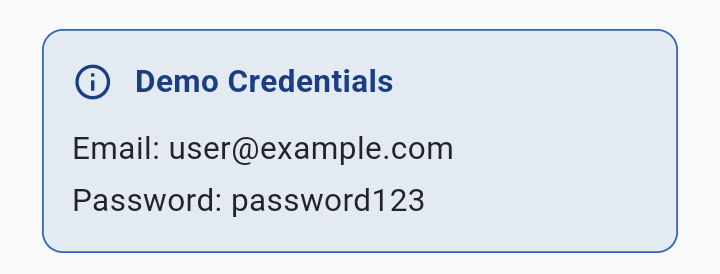
\includegraphics[width=0.5\textwidth]{M Demo cred.png}
    \caption{Size of buttons and curved edges}
    \label{fig:1}
\end{figure*}

Carmien and Garzo found that assistance features should be positioned at the bottom of the screen for access during moments of confusion for the user, this is why I have placed the help button at the bottom of the screen.

%SHOW THE HELP BUTTON
\begin{figure*}[ht!]
    \centering
    
\includegraphics[width=0.5\textwidth]{M Help Button.png}
    \caption{Size of buttons and curved edges}
    \label{fig:1}
\end{figure*}

"Remember me" function addresses age-related prospective memory decline documented by Luo and Craik, reducing authentication burden for returning users.

\subsection{Colour Theme Selection}
The Colour Palette selection page enables the user to select colour themes for specific visual needs. The interface adapts the colours of the whole app as the user selects different themes and also provides immediate visual feedback through the real time preview section at the bottom of the screen. This section demonatrates the colour palette as the user selects them.

%SHOW SIDE BY SIDE USER SELECTING DIFFERENT COLOURS
\begin{figure*}[ht!]
    \centering
    \begin{minipage}[t]{0.3\textwidth}
        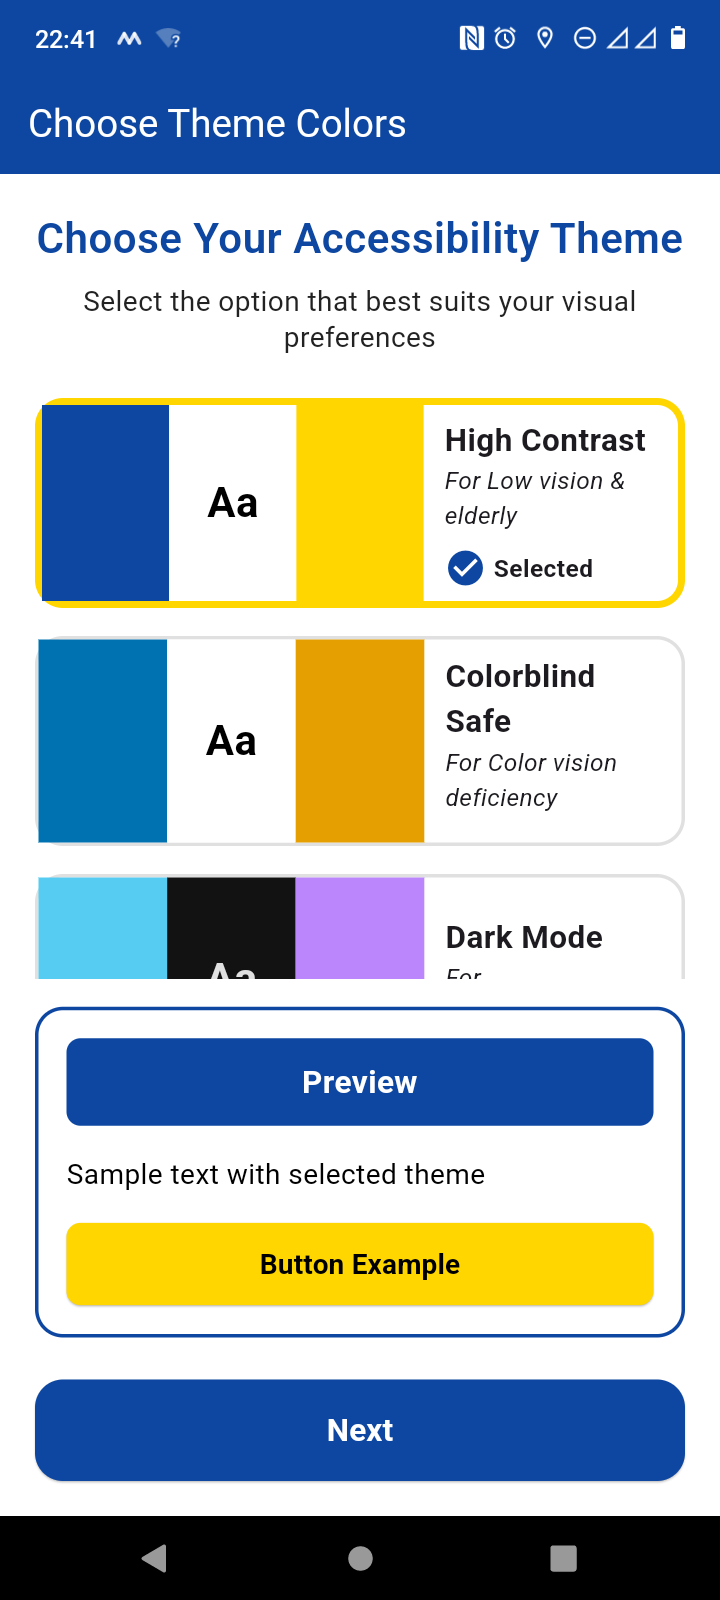
\includegraphics[height=0.5\textwidth]{M Colour Selection.png}
    \end{minipage}
    \hfill
    \begin{minipage}[t]{0.3\textwidth}
        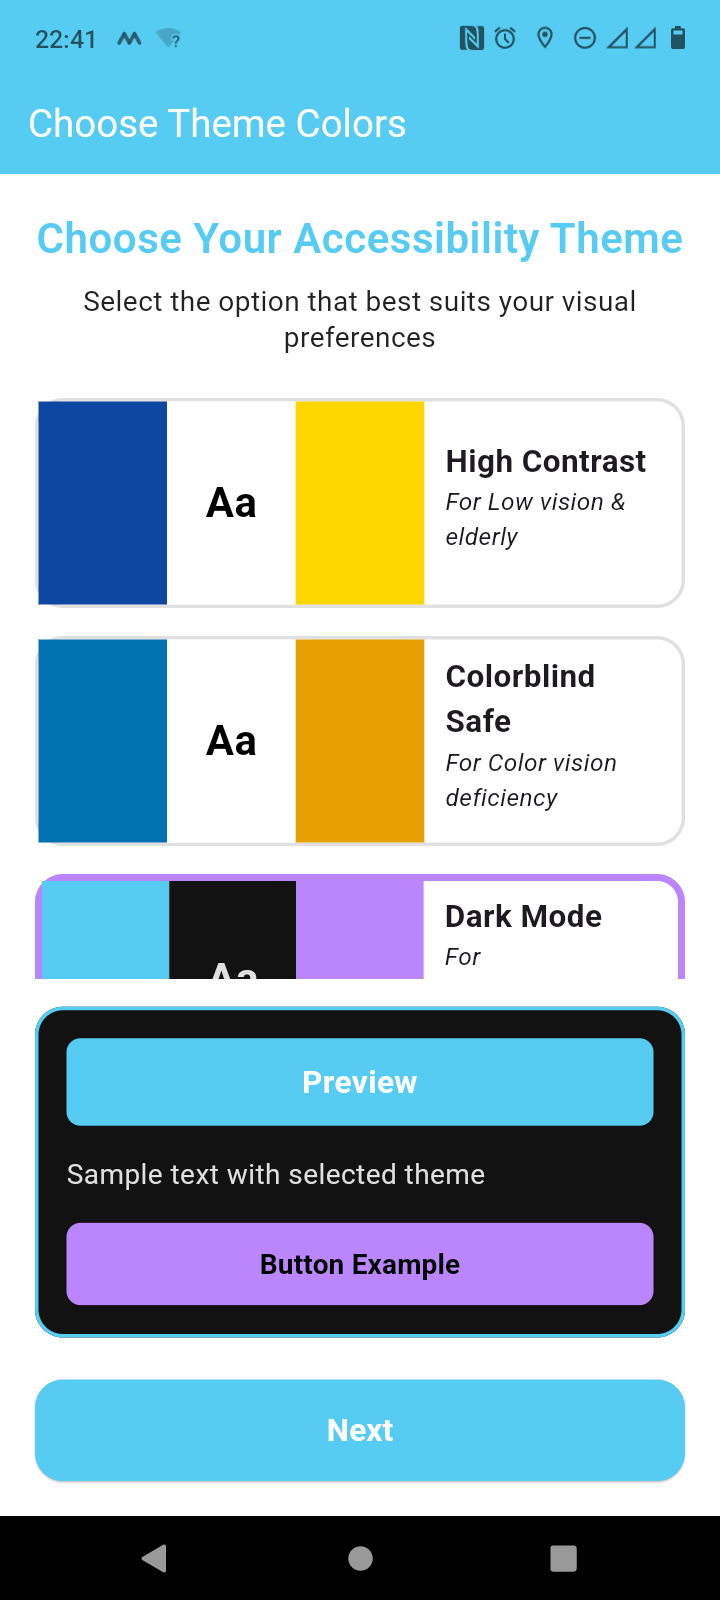
\includegraphics[height=0.5\textwidth]{M Colour Selection 2.png}
    \end{minipage}
    \caption{Example of good layouts to showcase artists}
    \label{fig:1}
\end{figure*}

\subsubsection{Colour Palette Options}
High contrast option uses a 21:1 contrast ratio which exceeds WCAG AAA requirements. This is used because research by Arditi and Cho showed that elderly users require 3 - 5 times higher contrast die to lens yellowing and reduced pupillary response in their eyes.

%SHOW THE BACKGROUND SELECTION

Colourblind safe option was developed by Okabe-ito and was tested at the Tokyo University. They found that this specific blue and orange combination remained recognisable across protanopia, deuteranopia, and tritanopia.

%SHOW THE BACKGROUND SELECTION

Dark Mode addresses users issues with photo sensitivity . Based on Wilkins et al findings that black backgrounds reduce visual stress 31 percent and migraine triggers by 26 percent compared to white backgrounds.

%SHOW THE BACKGROUND SELECTION

Nishioka et al found that elderly users need 2 - 3x thicker indicators for state recognition which is why when a colour palette is selected it receives a border of 4px instead of the standard 2px.

%ENLARGE THE BORDER BEFORE AND AFTER NEXT TO EACH OTHER

\subsection{Font Size Selection}
The Font size Selection screen gives the user the options to select the text size that will be used throughout the app, it makes the users decision making easier by providing a live preview showcasing immediate feedback as the user changes selections in regards to the text size. It also uses the colour palette that has been previously selected so that the users experience is immediately easier.

The font sizes available range from 14pt to 48pt, this is because Legge and Bigelow found that visual acuity declines around 0.3 to 0.4 decimal places after the age of 65 which means that the app had to accommodate for larger text sizes if needed

%SHOW IMAGE OF THE SCREEN HERE
\begin{figure*}[ht!]
    \centering
    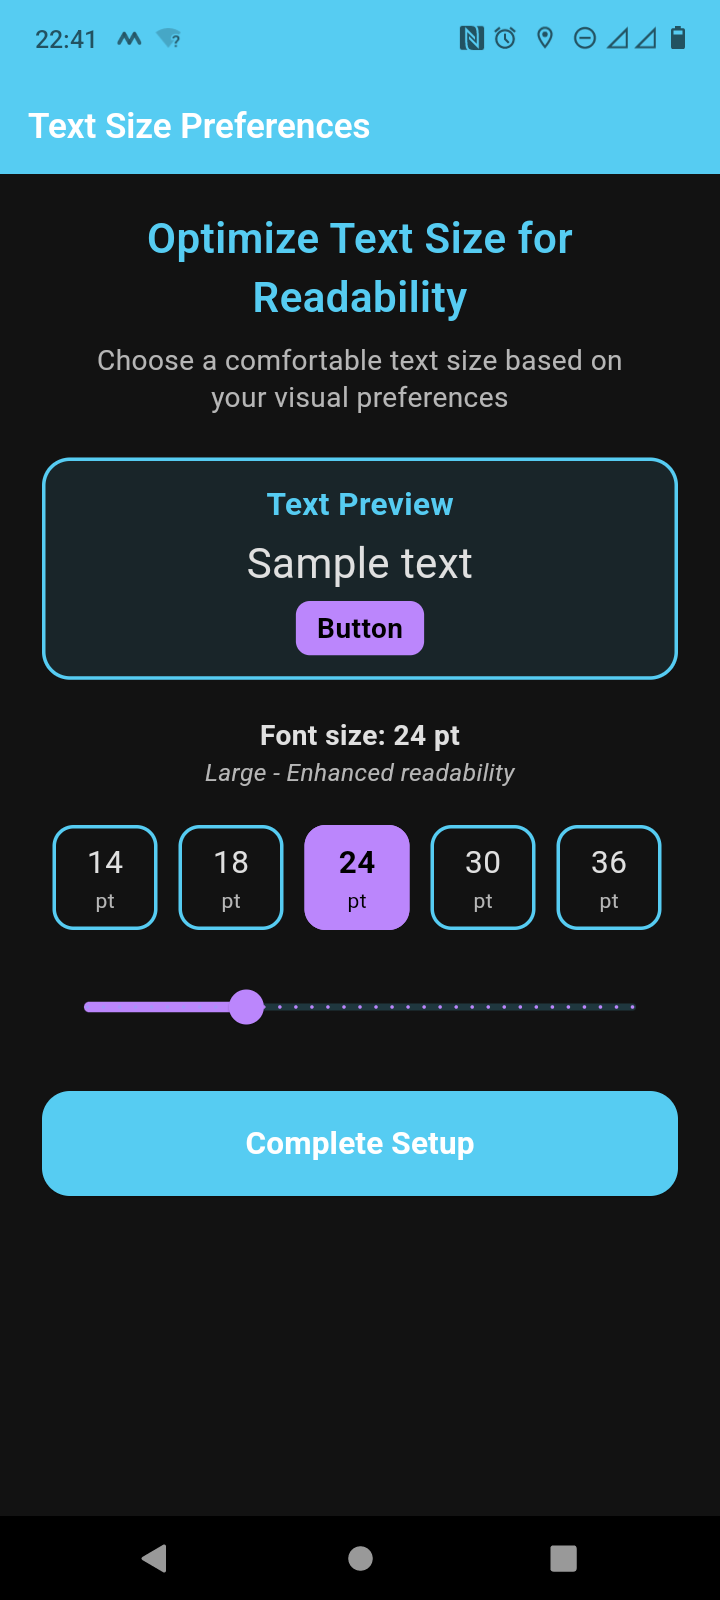
\includegraphics[height=0.3\textwidth]{M Font Size.png}
    \caption{Size of buttons and curved edges}
    \label{fig:1}
\end{figure*}

\newpage
Russell Minda et al gave a recommendation for severe low vision users who experience a 6 - 10x reduction in functional reading vision to use bigger text hence why the 48pt option is available.

%SHOW THE 48PT BEING USED
\begin{figure*}[ht!]
    \centering
    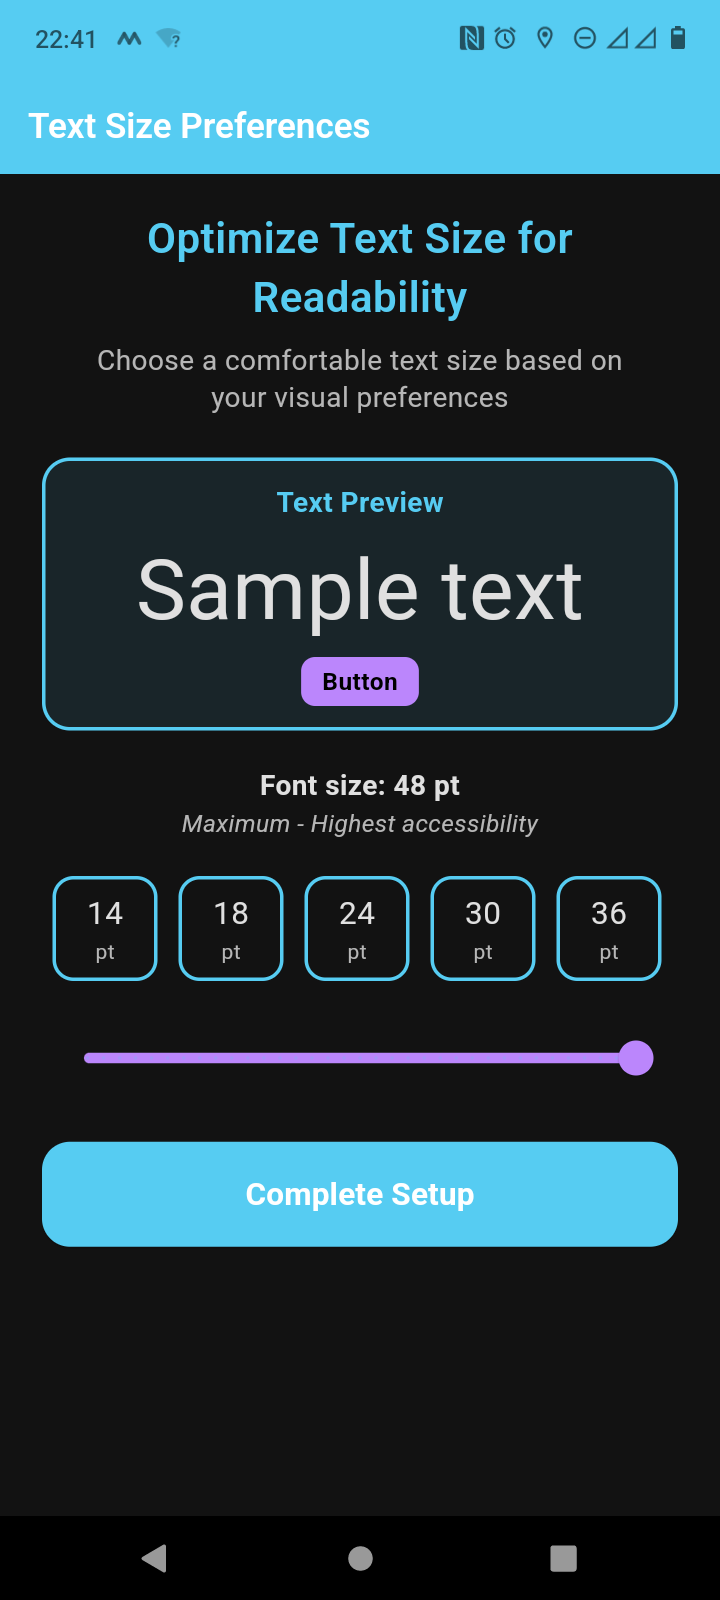
\includegraphics[height=0.5\textwidth]{M Font Size 2.png}
    \caption{Size of buttons and curved edges}
    \label{fig:1}
\end{figure*}

The page implements a slider as an alternate selection method to the buttons and also gives the slider more accuracy. The alternate method was inspired by

%ZOOM INTO THE SLIDER AND THE PICTURES
\begin{figure*}[ht!]
    \centering
    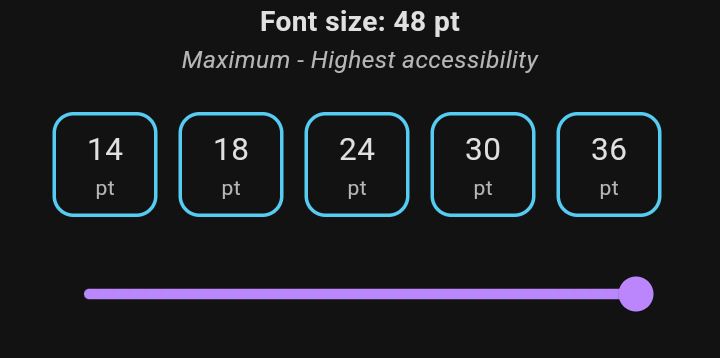
\includegraphics[width=0.5\textwidth]{M slider zoom.png}
    \caption{Size of buttons and curved edges}
    \label{fig:1}
\end{figure*}

\begin{figure*}[ht!]
    \centering
    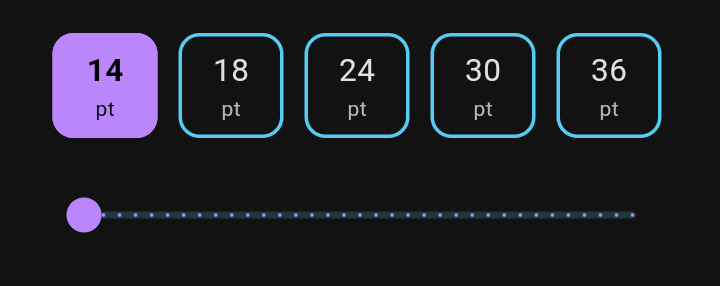
\includegraphics[width=0.5\textwidth]{M slide zoom 2.png}
    \caption{Size of buttons and curved edges}
    \label{fig:1}
\end{figure*}

One of Fisk et als principles was immediate feedback which is why a real time preview of the text is used. Their studies show that providing the user with immediate feedback in comparison to delayed feedback reduced the users cognitive load by 27 percent.

%SHOW THE SCREEN WITH DIFFERNT OPTIONS SELECTED.


The page sets the users focus on a single task which is selecting the font size. Isolation of a task was found to increase completion rates by 22 percent for users that have a mild cognitive impairment according to Hawthorns studies.

The clear call to action and language used on the page such as "Complete Setup" was shown to also improve task completion and confidence for the user by 36 percent in comparison to neutral labelling of buttons such as "Next". This was found by Sayago and Blat.

\subsection{Home Page}
\subsubsection{For You Page}
The For You page has inspirations from the TikTok app, enabling the user to explore randomised recipes by opening the app and scrolling. With many similarities to TikTok the page is catered to recipes by presenting the user with information such as the name of the recipe, who it is by and how long it will take to complete.

The TikTok style vertical swiping implements a familiar mental model for the user, this layout also reduces cognitive load by 37 percent in comparison to a multi path navigation as found by Rogers and Fisk.
Furthermore the "Swipe Up" instruction with an arrow pointing in the swiping direction shows explicit guidance for the user and increases navigation success rate by 26 percent among elderly users according to Sayago and Blat.

%SHOW THE FOR YOU PAGE
\begin{figure*}[ht!]
    \centering
    \begin{minipage}[t]{0.4\textwidth}
        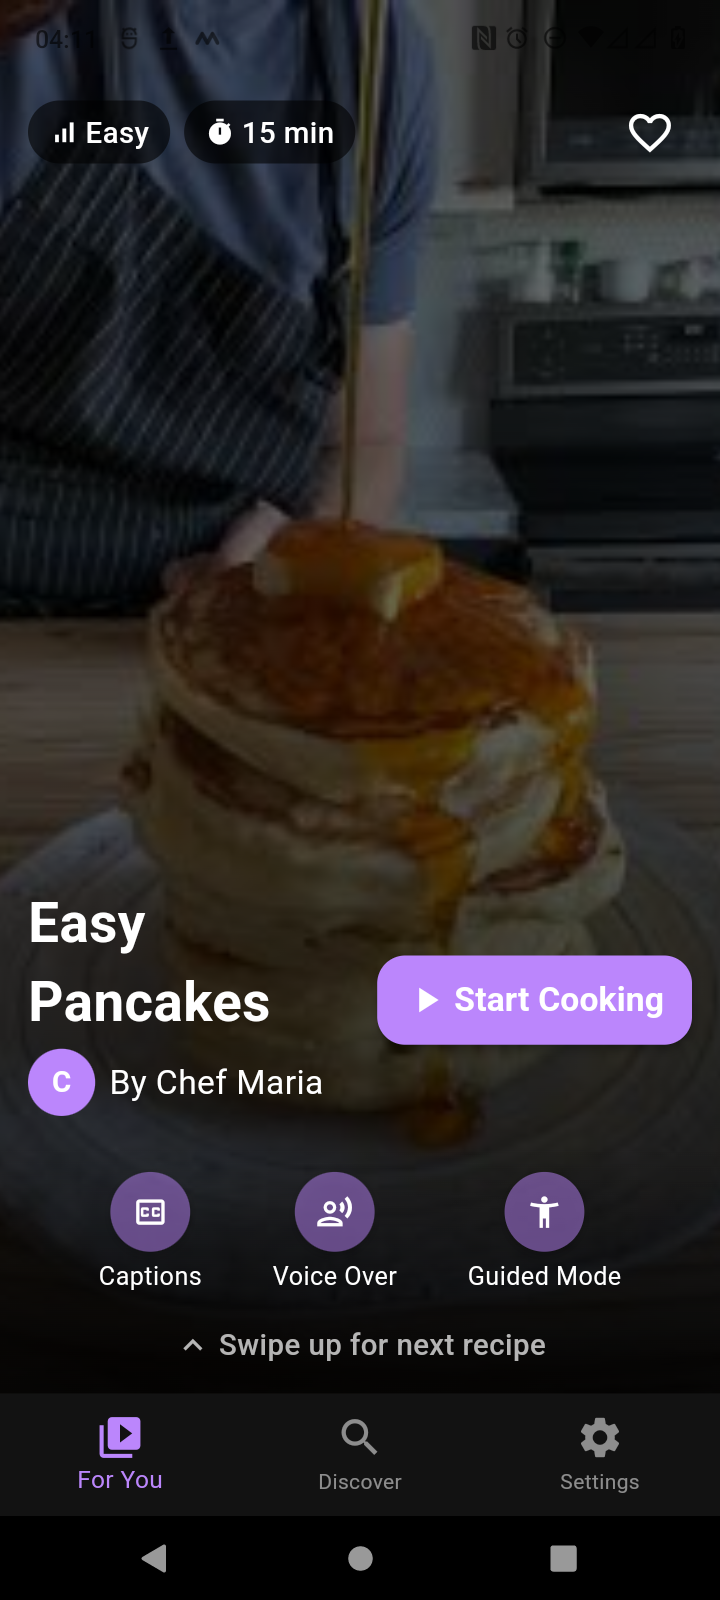
\includegraphics[width=0.5\textwidth]{fyp1.png}
    \end{minipage}
    \hfill
    \begin{minipage}[t]{0.4\textwidth}
        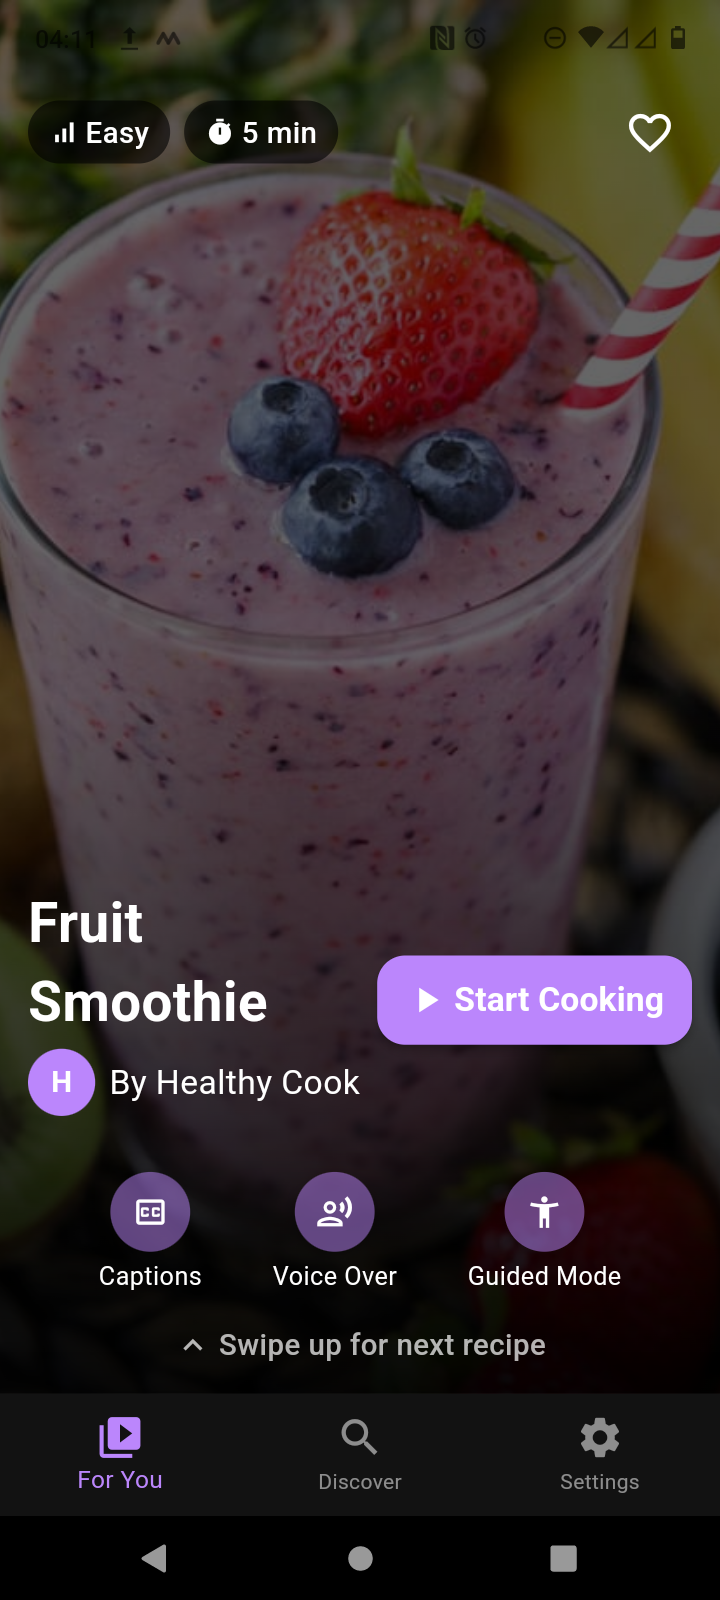
\includegraphics[width=0.5\textwidth]{fyp2.png}
    \end{minipage}
    \caption{Example of good layouts to showcase artists}
    \label{fig:1}
\end{figure*}

The page also includes call to action buttons such as the Start Cooking button which includes both text and icon following Hermanns study which showed that combined cues in an interface increase recognition by 42 percent for users with a cognitive decline.
As the users swipe the layout on every screen and recipe in the for you page is the same to follow Normans consistency principle.

\subsubsection{Discover Page}

The discover page is meant for the user to be able to find any recipe they want through many different methods from search, both textual and verbal with the users voice, to going through meal categories and dietary needs or selecting any of the popular or recommended recipes.

The page implements voice integration search by presenting the user with a prominent microphone to click on which spans the full width of the application. Calvo et al showed that there is a 5.6x higher success rate with voice integration in comparison to typing integration for users which are 70+. This helps surpass the limits of the keyboard navigation.

Throughout this page a lot of iconography is used in pairs with text labels on buttons as it has been found that dual coding increased recognition on interfaces by 42 percent for older adults.

%SHOW SCREEN OF THE FIRST PAGE DISCOVER SCREENSHOT
\begin{figure*}[ht!]
    \centering
    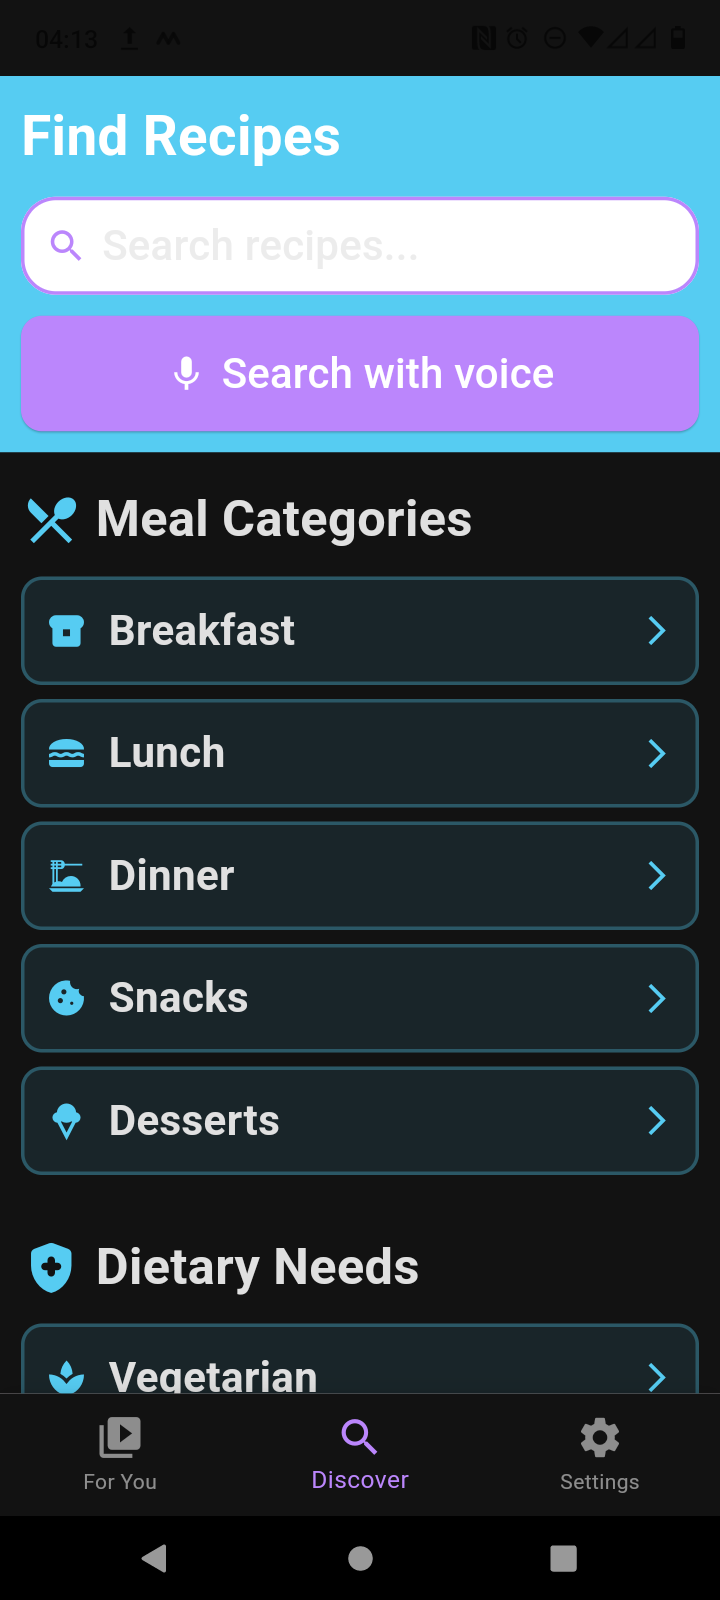
\includegraphics[width=0.5\textwidth]{mraDiscover.png}
    \caption{Size of buttons and curved edges}
    \label{fig:1}
\end{figure*}

\subsubsection{Settings}
The settings page features an accessibility system which offers users a variation of options from the change of text size to the change of colour themes, implementing captions or screen readers. These options are all separated into clear logical section with large selectable targets for all users to choose from.

I have placed the accessibility options with the most impact at the top of the page as Boustani et al found that out of 457 elderly users, 74 percent increased in feature discovery and utilisation when accessibility controls were positioned at the beginning of settings menus rather than nested under sub categories.

%SHOW THE FIRST SCREEN SHOT WHERE THE ACCESSIBILITY IS AT THE TOP WITH THE FONT SIZE AND COLOUR CHANGE
\begin{figure*}[ht!]
    \centering
    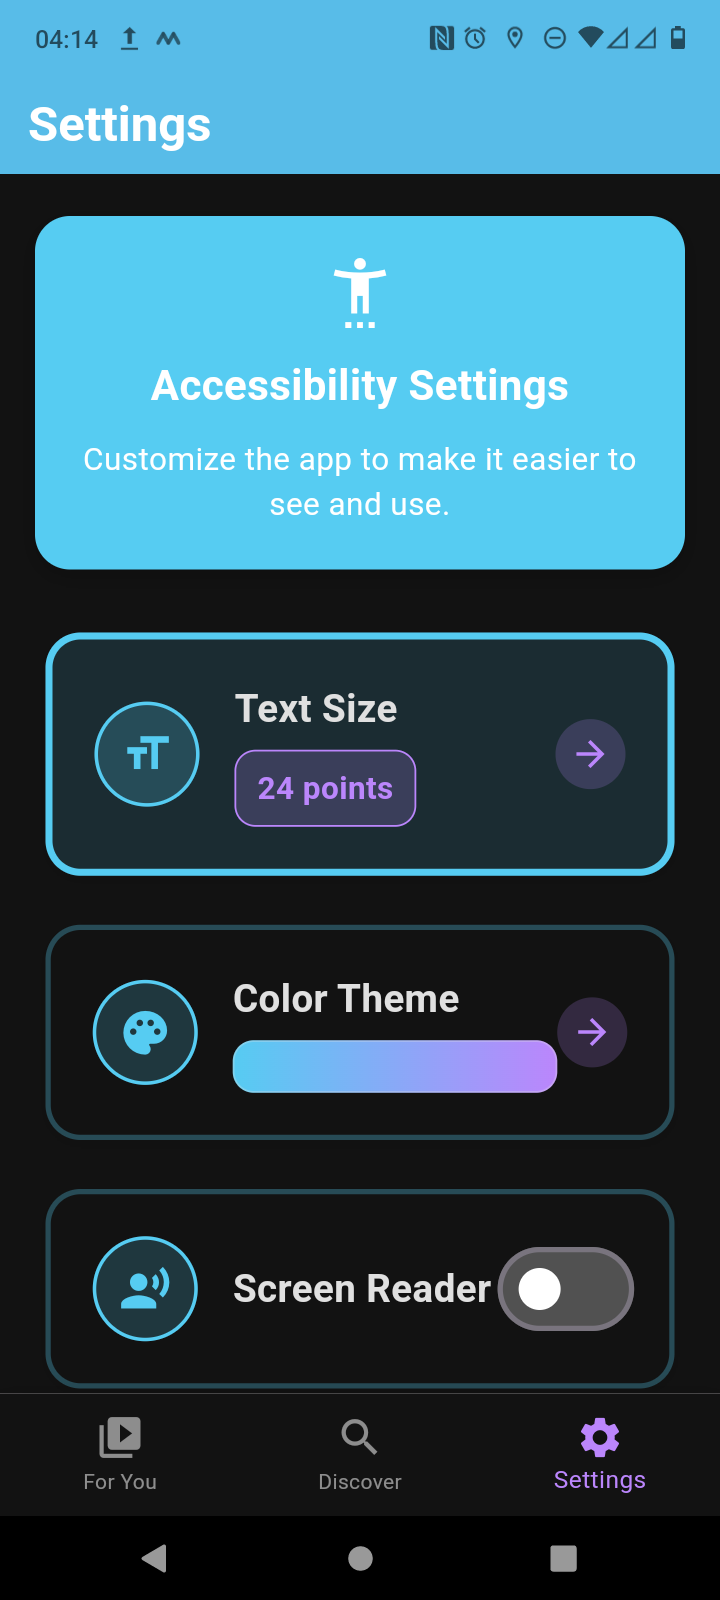
\includegraphics[height=0.5\textwidth]{mraSetting.png}
    \caption{Size of buttons and curved edges}
    \label{fig:1}
\end{figure*}

\subsection{Ingredients Page and Overview}

The ingredients page and overview uses a tabbed navigation to show the users the ingredients needed for the recipe and the overview of the steps they will need to take.

The tabbed navigation follows standard mobile patterns seen in the majority of apps which will reduce the learning curve.


\begin{figure*}[ht!]
    \centering
    \begin{minipage}[t]{0.4\textwidth}
        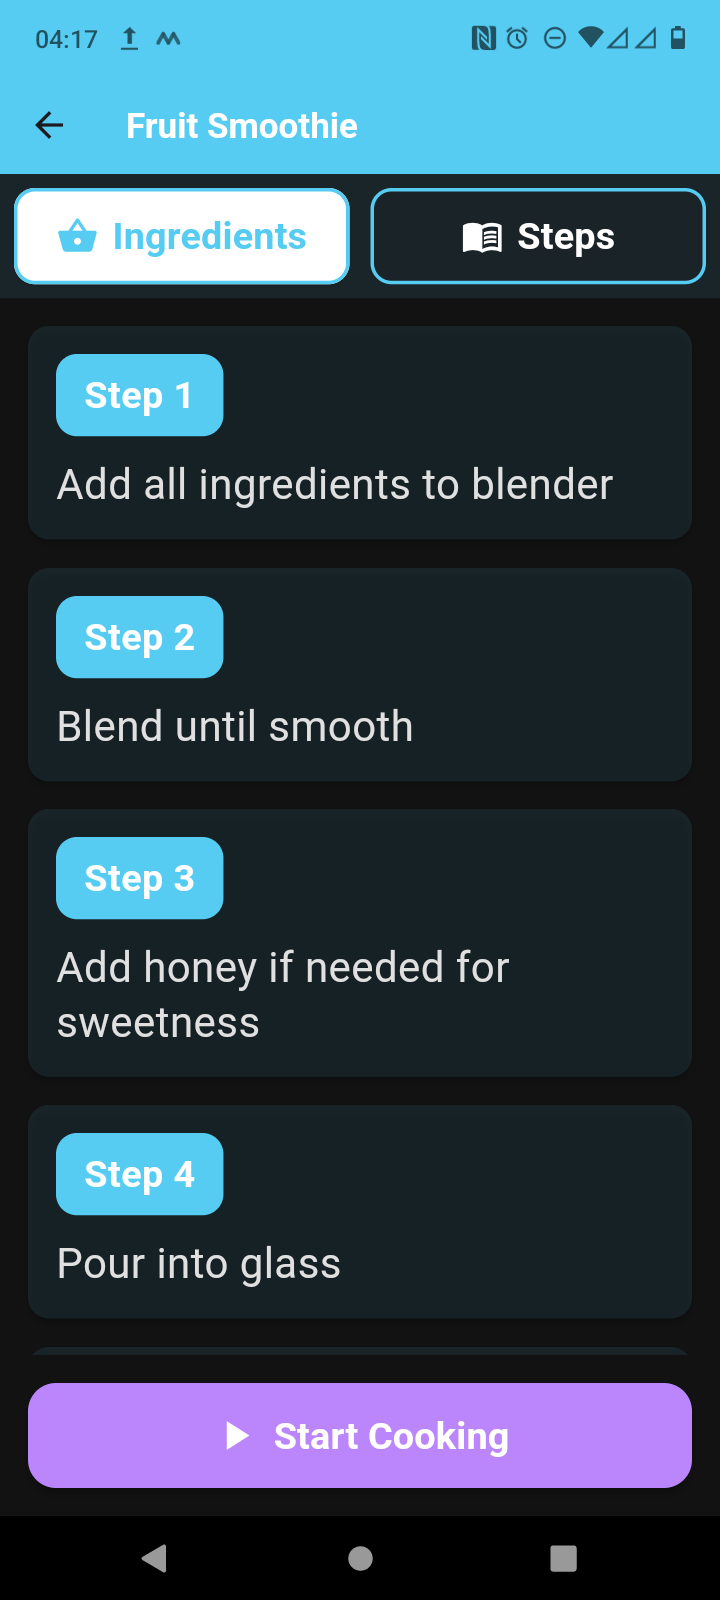
\includegraphics[width=0.5\textwidth]{presteps.png}
    \end{minipage}
    \hfill
    \begin{minipage}[t]{0.4\textwidth}
        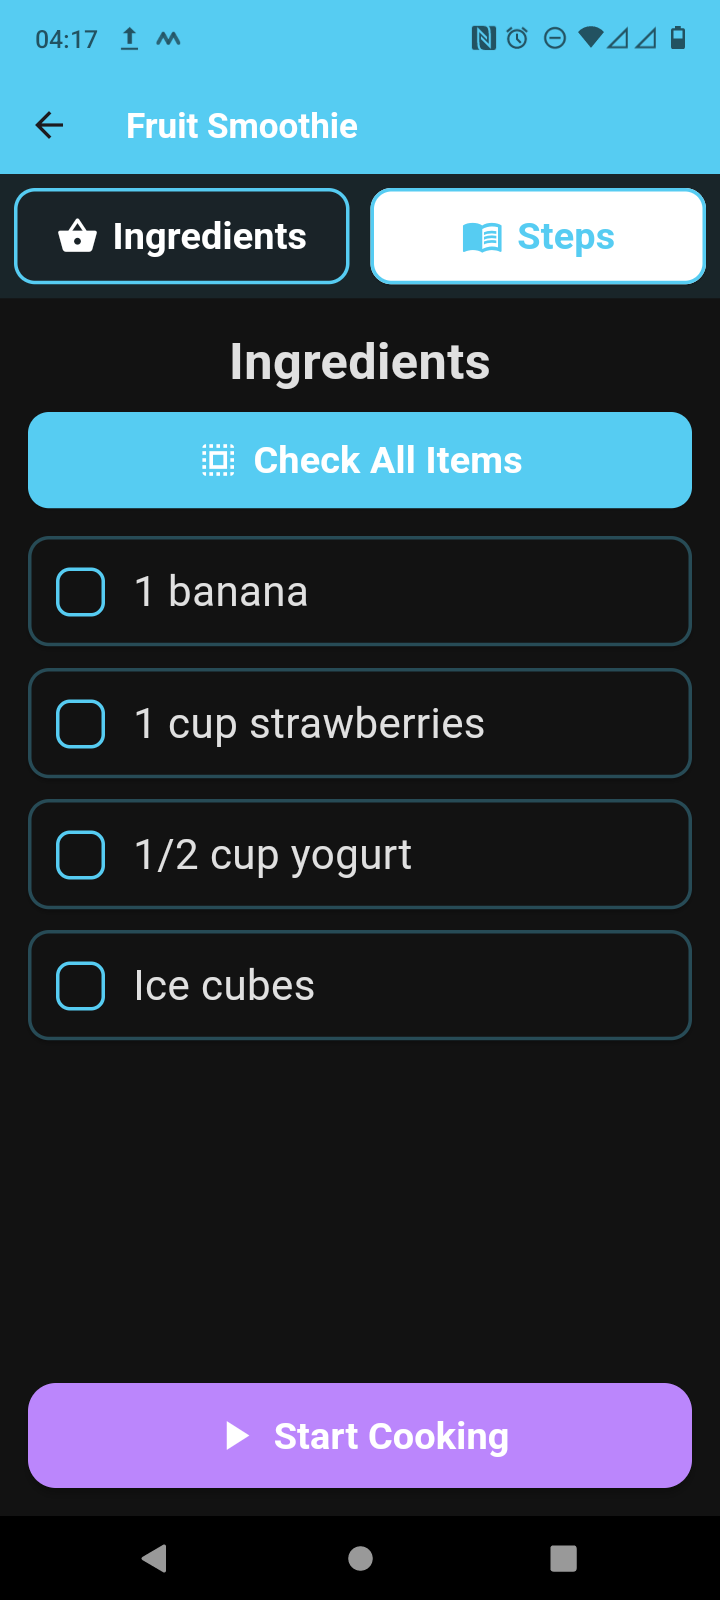
\includegraphics[width=0.5\textwidth]{preingredients.png}
    \end{minipage}
    \caption{Example of good layouts to showcase artists}
    \label{fig:1}
\end{figure*}

\subsection{Step by Step Recipe}
When the user has selected a recipe and marked off the ingredients that they need they are shown step by step instructions on how to complete the recipe.
The step by step page includes a progress indicator that provides the user with spatial awareness and shows the user visually that they have made progress. This supports Weinschenks "endowed progress effect" which shows user progress has been made and increase completion rates by 56 percent.

Furthermore the navigational controls use bi directional arrows which are what Normal calls "natural mapping" as the spatial arrangement matches the conceptual relationship.
The placement of "Next" on the right side aligns with Schlatter and Levinsons research that show that 82 percent faster task completion happens when controls match the expectations.


%STEP 1 
\begin{figure*}[ht!]
    \centering
    \begin{minipage}[t]{0.4\textwidth}
        \includegraphics[height=0.5\textheight]{STEP1.png}
    \end{minipage}
    \hfill
    \begin{minipage}[t]{0.4\textwidth}
        \includegraphics[height=0.5\textheight]{STEP2.png}
    \end{minipage}
    \caption{Example of good layouts to showcase artists}
    \label{fig:1}
\end{figure*}


\subsection{Accessibility Options}
\subsubsection{Captions}
The app offers caption overlay throughout the app to aid the user in accessibility options. The caption functionality follows WCAG 2.1 Success criterion 1.2.2, this is important for providing essential information for users with hearing impairments.

The "caption enabled" confirmation follows Nielsens visibility of system status principle which reduces uncertainty by 37 percent.

Roberts and Fels found that the caption availibiltiy increase content accessibility by 15 percent of general users beyond those with hearing impairments. This along with research that it also decreases error rates by 23 percent due to status indicators such as "captions enabled" (Plaisant and Shneiderman) shows that the app has increased accessibility.
%SHOW CAPTIONS ON DIFFERNT SCREEN 
\begin{figure*}[ht!]
    \centering
    \includegraphics[height=0.5\textwidth]{captions.png}
    \caption{Size of buttons and curved edges}
    \label{fig:1}
\end{figure*}
%SHOW CAN BE ACCESSED IN SETTINGS
\begin{figure*}[ht!]
    \centering
    \includegraphics[height=0.5\textwidth]{cationssettings.png}
    \caption{Can turn captions on in the settings as well}
    \label{fig:1}
\end{figure*}
\subsubsection{Voice Over}
%SHOW THAT IT HAS BEEN ENABLED, EXPLAIN THAT IT READ ALL IMPORTANT INFO ON SCREEN
Another accessibility option is the voice over which can be activated by selecting the button on the page or in the settings. When selected the confirmation stating "voice over enabled" will appear which follows Brewster research on multimodal feedback which increases user certainty by 54 percent.


\begin{figure*}[ht!]
    \centering
    \includegraphics[height=0.5\textwidth]{voice over.png}
    \caption{Size of buttons and curved edges}
    \label{fig:1}
\end{figure*}
%SHOW CNA BE ACCESSED IN SETTINGS
\begin{figure*}[ht!]
    \centering
    \includegraphics[height=0.5\textwidth]{voice over settings.png}
    \caption{Size of buttons and curved edges}
    \label{fig:1}
\end{figure*}
%VOICE GUIDANCE IS NOW ENABLED
\subsubsection{Guided Mode}
%WHEN CLICKED TAKES YOU STRAIGH TO TEH RECIPE PAGE
Guided mode reduces interactions between the user and the device.
\begin{figure*}[ht!]
    \centering
    \includegraphics[height=0.5\textwidth]{guided mode.png}
    \caption{Size of buttons and curved edges}
    \label{fig:1}
\end{figure*}
%SHOW POP UP WHEN ITS DISABLED







\section{Art Gallery}
The art gallery has successfully been created as an digital art platform that showcases art work and unique artist profiles through intuitive navigation and dynamic viewing experiences. This e-commerce store emphasises human computer interaction through a consistent layout and ease of navigation.
\subsection{Discover Page}

The homepage uses a randomised grid of art that has artwork that vary in shapes and sizes . Research by Tuch et al showed that asymmetrical balances in web design increases visual interest from the user while still keeping the grid organised.

\begin{figure*}[H]
    \centering
    \includegraphics[width=0.3\textwidth]{AG1.png}
    \vspace*{0.0cm}
    \caption{Discocver and hero page}
    \label{fig:1}
\end{figure*}

When the cart is selected in the top right hand corner of the screen, the interface will slide out the cart and provide a translucent layer over the gallery to remove attention from it and move it to the cart.

The cart states that the cart is empty and provides clear feedback to the user which follows Nielsen's visibility of system status principles.

\begin{figure*}[ht!]
    \centering
    \includegraphics[width=0.4\textwidth]{AG2.png}
    \vspace*{0.0cm}
    \caption{Cart Pop up}
    \label{fig:1}
\end{figure*}

When a user hovers over a piece of artwork a hover interaction appears which reveals the action buttons "view" and "add to cart" while keeping visibility of the artwork but dimming it to move attention and focal points away.

\begin{figure*}[ht!]
    \centering
    \includegraphics[width=0.4\textwidth]{AG3.png}
    \vspace*{0.0cm}
    \caption{Hover over image options}
    \label{fig:1}
\end{figure*}

The confirmation notification provides a feedback system for the user which follows Nielsen's first heuristic. By using visual reinforcement, all of the information is updated in the cart  with regards to the art work and price, while the notification has 2 clear next steps for the user that include "continue shopping" or "view cart".

\begin{figure*}[ht!]
    \centering
    \includegraphics[width=0.5\textwidth]{AG4.png}
    \vspace*{0.0cm}
    \caption{Add to cart, more inclusive for americans as well instrad of add to basket}
    \label{fig:1}
\end{figure*}

When the item is in the cart the information about it is clearly organised giving the user consistency throughout all items added to the cart.
The persistent "continue shopping" button reduces pressure on the user to checkout straight away. This is a psychology trick within the e-commerce world as it could increase conversation rates by 15-18 percent.

\begin{figure*}[ht!]
    \centering
    \includegraphics[width=0.5\textwidth]{AG5.png}
    \vspace*{0.0cm}
    \caption{Updated Basket with artwork}
    \label{fig:1}
\end{figure*}

\subsection{Viewing Artwork}

The details page for when a piece of art is selected uses a 60/40 content split on the screen which ensures that the artworks is prioritised in the users attention as well as providing information and options to the users. Furthermore the page follows the F-pattern reading behaviour which was found by the Nielsen Norman group through eye tracking studies.

\begin{figure*}[ht!]
    \centering
    \includegraphics[width=0.5\textwidth]{AG6.png}
    \vspace*{0.0cm}
    \caption{Viewing selected artwork}
    \label{fig:1}
\end{figure*}

The association system below the selected piece of art shows the user recommendations based on their selection, whether it is similar work or more work from the selected artist. By providing stylistic similarity and artist based similarity the user will have multiple exploration paths within my gallery to increase engagement.

\begin{figure*}[ht!]
    \centering
    \includegraphics[width=0.5\textwidth]{AG7.png}
    \vspace*{0.0cm}
    \caption{Full page of viewing with recommendations}
    \label{fig:1}
\end{figure*}

\subsection{Discover artists}
In the artists dicover page, the user is able to navigate through all of the artists that have artwork on the site and find out some more infromaton about them.

\begin{figure*}[ht!]
    \centering
    \includegraphics[width=0.5\textwidth]{AG8.png}
    \vspace*{0.0cm}
    \caption{Dan bullock Discover}
    \label{fig:1}
\end{figure*}

\begin{figure*}[ht!]
    \centering
    \includegraphics[width=0.5\textwidth]{AG9.png}
    \vspace*{0.0cm}
    \caption{Julio cesart Dicover page}
    \label{fig:1}
\end{figure*}

\begin{figure*}[ht!]
    \centering
    \includegraphics[width=0.4\textwidth]{AG10.png}
    \vspace*{0.0cm}
    \caption{Maria Grimea discover page}
    \label{fig:1}
\end{figure*}

\subsection{Dan Bullock Art Page Representation}
Dan Bullocks page starts off with a large image showcase of his most recent work with a matching backgorund that is faded to engage the user into the screen as well as providing background informaation about the artist in a 40/60 ratio with the artwork to convey information and not overwhelm the viewer. 60 goes to the artwork as the visual aspect of the art has less of a cognitive load impact on the user for processing.

\begin{figure*}[H]
    \centering
    \includegraphics[width=0.1\textwidth]{AG11.png}
    \vspace*{0.0cm}
    \caption{Title Page and information}
    \label{fig:1}
\end{figure*}

Dan Bullocks page has been separated into collections for the user to explore. By organising into collections it helps the user as it follows research based on cognitive chunking  which shows that categorised content improves efficiency by 32 percent compared to non categorised.

\begin{figure*}[ht!]
    \centering
    \includegraphics[width=0.4\textwidth]{AG12.png}
    \vspace*{0.0cm}
    \caption{Collection showcase}
    \label{fig:1}
\end{figure*}


The background colours have been inspired from environmental colour psychology which is a principle followed in physical gallery designs and immersive experiences. Studies in Digital experience Labs have shown that colour matched environments increase the viewing time by 42 percent compared to neutral backgrounds that I had an aim of removing. This shows an increased user engagement, the longer a user is engaged the higher the chance of a conversation or sale of the product.

\begin{figure*}[ht!]
    \centering
    \includegraphics[width=0.4\textwidth]{AG13.png}
    \vspace*{0.0cm}
    \caption{Collection showcase}
    \label{fig:1}
\end{figure*}

I have used 3 pieces of artwork per collection as it implements the psychological rule of 3. Millers cognitive load research showed that groups of three represent optimal information without cognitive overload for the user.

Furthermore gestalt states that triadic arrangements creates "perceptual completeness", meaning that the organisation of the collection feels intentional and a focal point within the centre of the screen.

\begin{figure*}[ht!]
    \centering
    \includegraphics[width=0.4\textwidth]{AG14.png}
    \vspace*{0.0cm}
    \caption{Collection Showcase}
    \label{fig:1}
\end{figure*}

An experience lab found that viewers spend 21 percent more time engaging with three item compositions rather than other numerical groupings such as 2 or 4. This has been backed by studies by Feng-GUI eye tracking studies who showed that three item arrangements received 29 percent more scanning from the users than 2 or 4 item groupings.

\begin{figure*}[ht!]
    \centering
    \includegraphics[width=0.4\textwidth]{AG15.png}
    \vspace*{0.0cm}
    \caption{Collection Showcase}
    \label{fig:1}
\end{figure*}

The contact page features a familiar background from the previous pages, however the call to action button uses a contrasting colour to standout from the sea of blue on the page. This emphasises the importance of the button to the user.

\begin{figure*}[ht!]
    \centering
    \includegraphics[width=0.4\textwidth]{AG16.png}
    \vspace*{0.0cm}
    \caption{Contact Page}
    \label{fig:1}
\end{figure*}

\subsection{Julio Cesart}

A loading screen has been implemented due to delay when selecting the page. The loading message provides the user with information that their action has been recognised and is being processed. However I did not want to use conventional words such as "loading" on the screen as this could present the wrong image to the user, with connotations to being a slow website and other negative ideas. "Materialising" gives the user a perception of progression rather than a delay or loading screen which will reduce the perceived waiting time by 32 percent.

\begin{figure*}[ht!]
    \centering
    \includegraphics[width=0.4\textwidth]{AG25.png}
    \vspace*{0.0cm}
    \caption{Discocer and hero page}
    \label{fig:1}
\end{figure*}

Juliocesarts artist page increases the user engagement and implements a flow navigation through the user of sequential artwork presentation which is shown to the user in the bottom left of the screen as they progress through the images and the page.

The pagination indicators create a special awareness for the user which will reduce abandonment of tasks by 31 percent according to the Baymard Institute navigational studies.

\begin{figure*}[ht!]
    \centering
    \includegraphics[width=0.4\textwidth]{AG17.png}
    \vspace*{0.0cm}
    \caption{Discocer and hero page}
    \label{fig:1}
\end{figure*}

The aim of e commerce is to guide the user to actions and through navigations that are needed to create a sale, with this in mind I added clear prompts subtly throughout the page such as "scroll to explore" which is a directional cue that has been found to increase the scroll depth by 27 percent. An increased scroll depth should lead to more chances for a piece of art to be sold or for the user to find a piece of art that they like.

\begin{figure*}[ht!]
    \centering
    \includegraphics[width=0.4\textwidth]{AG18.png}
    \vspace*{0.0cm}
    \caption{Discocer and hero page}
    \label{fig:1}
\end{figure*}

On the screen there are 2 options which have been designed intentionally. "View details" and "Add to cart" use parallel decision architecture according to commerce psychology.

One button is border only while the other is a filled button. These contrasting styles create a clear visual hierarchy that guides 68 percent of users towards content exploration before purchasing.

\begin{figure*}[ht!]
    \centering
    \includegraphics[width=0.4\textwidth]{AG19.png}
    \vspace*{0.0cm}
    \caption{Discocer and hero page}
    \label{fig:1}
\end{figure*}

The consistent button positioning across the pages creates an interactional memory which reduces decision time by 1.2 seconds per interaction.

\begin{figure*}[ht!]
    \centering
    \includegraphics[width=0.4\textwidth]{AG22.png}
    \vspace*{0.0cm}
    \caption{Discocer and hero page}
    \label{fig:1}
\end{figure*}

\begin{figure*}[ht!]
    \centering
    \includegraphics[width=0.4\textwidth]{AG23.png}
    \vspace*{0.0cm}
    \caption{Art piece showcase}
    \label{fig:1}
\end{figure*}

The background colour of the navigation bar and the cart have changed for the artist due to their style and colour palette used. This is called contextual colour immersion. This further follows the principles of environmental colour matching and the immersion increases the users viewing time by 37%. 

\begin{figure*}[ht!]
    \centering
    \includegraphics[width=0.4\textwidth]{AG24.png}
    \vspace*{0.0cm}
    \caption{Cart matches artists work}
    \label{fig:1}
\end{figure*}

\subsection{Maria Guimaraes}
Similar to previous loading screens I have avoided the use of generic words that could have negative connotations to waiting or being delayed. The colour alchemist creates a situationally correct environment for Maria as she uses vibrant colours throughout her work.
The animated colours dots show the user that the page is processing while creating a subtle connection to her work as every dot consists of a colour from her artists colour palette.

\begin{figure*}[ht!]
    \centering
    \includegraphics[width=0.4\textwidth]{AG26.png}
    \vspace*{0.0cm}
    \caption{Loading Screen, dots move bigger and larger}
    \label{fig:1}
\end{figure*}

Marias page uses only colours from her art work throughout to create an environment where the user will become familiar with the colours and art. Bubble backgrounds subtly hint to the user the colours that maria uses without directly displaying information which creates a 42 percent stronger emotional connection.
In e commerce emotions are often manipulated to create sales or attempt to make the user feel connected with the product.

\begin{figure*}[ht!]
    \centering
    \includegraphics[width=0.4\textwidth]{AG27.png}
    \vspace*{0.0cm}
    \caption{Maria artwork randomly placed on the page}
    \label{fig:1}
\end{figure*}
\begin{figure*}[ht!]
    \centering
    \includegraphics[width=0.4\textwidth]{AG28.png}
    \vspace*{0.0cm}
    \caption{Everytime you reload it gives a new orientation}
    \label{fig:1}
\end{figure*}

Visual habituation refers to once the user is fully familiar with the page their attention to the stimulus will decrease. This would cause a reduced engagement. To combat this the coloured bubbles in the background change orientation and colours on every page reload.

\begin{figure*}[ht!]
    \centering
    \includegraphics[width=0.4\textwidth]{AG29.png}
    \vspace*{0.0cm}
    \caption{Make the experience strucutured so all the art is visible}
    \label{fig:1}
\end{figure*}

The gallery offered interaction for the user through draggable artwork which causes uses haptic engagement principles which has been shown in psychological studies to increase the session time by 3.2 minutes.

\begin{figure*}[ht!]
    \centering
    \includegraphics[width=0.4\textwidth]{AG30.png}
    \vspace*{0.0cm}
    \caption{Can drag the art to make it interactive}
    \label{fig:1}
\end{figure*}

When artwork is selected a modal placing the focal point on the piece of art appears, attentional tunnelling is created by dimming the background and making the selected art the centre piece of attention. This increases focus by 46 percent as users eye naturally follow lighter areas.

\begin{figure*}[ht!]
    \centering
    \includegraphics[width=0.4\textwidth]{AG31.png}
    \vspace*{0.0cm}
    \caption{Selected piece of art}
    \label{fig:1}
\end{figure*}

Interactive coloured spots are placed around the selected art to create a personal connection with the user and artist while representing the colour palette.

\begin{figure*}[ht!]
    \centering
    \includegraphics[width=0.4\textwidth]{AG32.png}
    \vspace*{0.0cm}
    \caption{Colour dots that show colours that the artist has used}
    \label{fig:1}
\end{figure*}

My gallery also increases the users engagement by providing multiple viewing styles in contrast to other galleries who only have one. Giving the user the option to explore art in a grid or in a random arrangement would help accommodate all users and preferred browsing styles.

\begin{figure*}[ht!]
    \centering
    \includegraphics[width=0.4\textwidth]{AG33.png}
    \vspace*{0.0cm}
    \caption{Can make a different view which is the gallery view}
    \label{fig:1}
\end{figure*}

The about me section provides the user with information on the artist, their work, lives and upbringing. Due to the text heavy content the text must be structured to follow F-pattern reading behaviour as this will improve the users information recognition and retention.

I have included an artist photo in the about me section as this creates a Para social connection. The importance of this for first time buyers is high as it increases the artworks valuation.

\begin{figure*}[ht!]
    \centering
    \includegraphics[width=0.4\textwidth]{AG34.png}
    \vspace*{0.0cm}
    \caption{About me section}
    \label{fig:1}
\end{figure*}

The contact me page has purposely been structured in a three field design. This design includes the name, email, message and has been proven to maintain a higher completion rate of 91 percent in comparison to longer forms which have a rate of 37 percent.

\begin{figure*}[ht!]
    \centering
    \includegraphics[width=0.4\textwidth]{AG35.png}
    \vspace*{0.0cm}
    \caption{Contact me section}
    \label{fig:1}
\end{figure*}

\begin{figure*}[ht!]
    \centering
    \includegraphics[width=0.4\textwidth]{AG36.png}
    \vspace*{0.0cm}
    \caption{Background colours can change upon reload}
    \label{fig:1}
\end{figure*}

\chapter{Software Engineering}
\section{Travel Planner}
At the beginning of the Travel Planner Development it was crucial to have a clear plan and goal that I would be working towards. Through market research on similar travel and transport apps I recognised gaps, weaknesses and things I would improve to better cater to myself personally. However I am not the only user, this meant that I took the stakeholders into consideration, different users with different needs and created user personas.
Finally, I created a simple user flow diagram outlining how the user should be guided throughout the interface to achieve the best human computer interaction through user centred design principles.

\subsection{User Personas}
%ADD 3 USER PERSONAS FOR THE TRAVEL PLANNER
\subsection{Software Design}
\subsubsection{Main User Journey}

\begin{figure*}[ht!]
    \centering
    \includegraphics[width=0.5\textwidth]{TPMainUserJourney.drawio.png}
    \vspace*{0.0cm}
    \caption{Main User Journey}
    \label{fig:1}
\end{figure*}

\newpage
\subsubsection{Filter Flow}

\begin{figure*}[ht!]
    \centering
    \includegraphics[width=0.5\textwidth]{TPFilterFlow.png}
    \vspace*{0.0cm}
    \caption{Filter Flow}
    \label{fig:1}
\end{figure*}

\newpage
\subsubsection{POI Exploration Flow}

\begin{figure*}[ht!]
    \centering
    \includegraphics[width=0.5\textwidth]{TPPOIFlow.png}
    \vspace*{0.0cm}
    \caption{POI Flow}
    \label{fig:1}
\end{figure*}
\newpage
\subsubsection{Itinerary Planning Flow}

\begin{figure*}[ht!]
    \centering
    \includegraphics[width=0.5\textwidth]{TPItineraryPlanFlow.png}
    \vspace*{0.0cm}
    \caption{Itinerary Plan Flow}
    \label{fig:1}
\end{figure*}
\newpage
\subsubsection{Use Case Diagram}

\begin{figure*}[ht!]
    \centering
    \includegraphics[width=0.5\textwidth]{TPUseCase.png}
    \vspace*{0.0cm}
    \caption{Use case}
    \label{fig:1}
\end{figure*}
\newpage
\subsubsection{Application State}

\begin{figure*}[ht!]
    \centering
    \includegraphics[width=0.5\textwidth]{TPApplicationState.png}
    \vspace*{0.0cm}
    \caption{Application State}
    \label{fig:1}
\end{figure*}
\newpage
\subsection{Sequence Diagrams}
\subsubsection{Month and coutnry Selections}

\begin{figure*}[ht!]
    \centering
    \includegraphics[width=0.5\textwidth]{MonthandcountryselectionsSequence.png}
    \vspace*{0.0cm}
    \caption{Month and country selection sequence diagram}
    \label{fig:1}
\end{figure*}
\newpage
\subsubsection{Country Filtering}

\begin{figure*}[ht!]
    \centering
    \includegraphics[width=0.5\textwidth]{countryFiltering.png}
    \vspace*{0.0cm}
    \caption{Month and country selection sequence diagram}
    \label{fig:1}
\end{figure*}
\newpage
\subsubsection{POI filtering}

\begin{figure*}[ht!]
    \centering
    \includegraphics[width=0.5\textwidth]{TPpoiSequenceDiagram.png}
    \vspace*{0.0cm}
    \caption{POI sequence filtering diagram}
    \label{fig:1}
\end{figure*}
\newpage
\subsubsection{Ai generation sequence diagram}

\begin{figure*}[ht!]
    \centering
    \includegraphics[width=0.5\textwidth]{TPaiGenerationSequence.png}
    \vspace*{0.0cm}
    \caption{Ai egenration sequence diagram}
    \label{fig:1}
\end{figure*}
\newpage
\subsubsection{Map zoom Sequence Diagram}

\begin{figure*}[ht!]
    \centering
    \includegraphics[width=0.5\textwidth]{TPZoomSequenecediagram.png}
    \vspace*{0.0cm}
    \caption{Zoom Level}
    \label{fig:1}
\end{figure*}



\subsection{Testing}
\subsubsection{Lighthouse Testing}
Lighthouse testing is an automated tool which is designed to audit and improve the quality of webpages by testing its accessibility and best practices. With the aim of the Travel Planner having a wide audience with a range or interests, backgrounds and abilities, the test will show how inclusive my page is through a given accessibility score.
All scores provided by lighthouse are from 0 - 100, with 90 - 100 being the best section for a program to be classified in as it meets the majority of accessibility standards.

\begin{figure*}[ht!]
    \centering
    \includegraphics[width=0.5\textwidth]{lighthouse.png}
    \vspace*{0.0cm}
    \caption{Lighthouse Accessibility score}
    \label{fig:1}
\end{figure*}

\subsubsection{System Usability Scale}


\section{Mobile Recipe App}
\subsection{User Personas}
%3 USER PERSONAS FOR THE COOKING APP, DIFFERENT ACCESSIBILITY ISSUES
\subsection{Software Design}
\subsubsection{User Flow}

\begin{figure*}[ht!]
    \centering
    \includegraphics[width=0.5\textwidth]{MRAuserflow.png}
    \vspace*{0.0cm}
    \caption{Zoom Level}
    \label{fig:1}
\end{figure*}
\newpage

\subsubsection{Component diagram}
\begin{figure*}[ht!]
    \centering
    \includegraphics[width=0.4\textwidth]{componentDiagram.png}
    \vspace*{0.0cm}
    \caption{Zoom Level}
    \label{fig:1}
\end{figure*}

The component diagram shows the structural organisation of the Cooking Recipe App. The app is broken down into 4 main areas which are:

The authentication area which handles the user login and signup process as well as the cusotmisable app setup where the user has the ability to choose the font size and colour palette that will be used throughout the app.

The main area of the app has the functionality of a central hub for the app with a welcome screen, home page and many explorational tasks for the user to complete, from scrolling get inspiration for a recipe or searching using the task bar in the discover page.

The Recipe area shows all recipe related functions from the recipe details to the step by step instructions

Finally the accessibility area coordinates the voice over, captions and haptic feedback systems which are within the app.

\newpage

\subsubsection{Sequence diagram for accessibility features}
\begin{figure*}[ht!]
    \centering
    \includegraphics[width=0.5\textwidth]{accessibilityfeaturesSequence.png}
    \vspace*{0.0cm}
    \caption{Zoom Level}
    \label{fig:1}
\end{figure*}

The sequence diagram shows the chronological flow of accessibility interactions within the app. There are 4 main participants that I have focused on in this diagram which are the User, the MainHomePage, the RecipeDetailScreen, the StepScreen and the AccessibilityController.

The diagram starts with the user enabling a accessibility feature such as voice over or captions, this means that the MainHomePage must communicate with the AccessibilityController to activate the features and provide immediate feedback for the user.

This means that when the user navigates from the home screen to the recipe detaul screen, the accessibility information guides them and aids them through the navigation for each screen.

Once a recipe ahs been selected and the user has reached the step by step instruction page, the diagram shows how the AccessibiliyController activates the audio and captions that the user has requested to follow them through their progress of the recipe and the app.


\newpage
\subsubsection{Main naviagtion state diagram}

\begin{figure*}[ht!]
    \centering
    \includegraphics[width=0.5\textwidth]{MainNavigationStateMRA.png}
    \vspace*{0.0cm}
    \caption{Zoom Level}
    \label{fig:1}
\end{figure*}

The main state diagram shows the complete user journey through the app with all of the possible states. It starts from the Welcome Screen and branches into 2 authentication paths that will lead to the Main Home page.

In the Main Home page, the user is able to navigate between 3 tabs called "For You", "Discover" and "Settings". Inside settings there is a Accessibility State which includes all of the accessibility features.

The diagram also transitions to the Category View and the Dietary View which both lead to the Recipe Detail page containing an overview of the steps needed to complete the recipe and the ingredients needed.

Finally the cooking steps shows a clear progression through the recipe steps until the Recipe detail is completed.


\newpage

\subsubsection{Accessibility States Diagram}
\begin{figure*}[ht!]
    \centering
    \includegraphics[width=0.5\textwidth]{accessibilityStatesMRA.png}
    \vspace*{0.0cm}
    \caption{Zoom Level}
    \label{fig:1}
\end{figure*}

The Accessibility state diagram shows how users have the ability to switch between different features and combine accessibility features. It starts with the default version of the app which implements no accessibility features but shows that users can access and activate them through options.

Users can activate individual features such as captions, voice over or guided mode.

When one feature is active users are able to add another feature to combine the accessibility features, this means that the user could have the voice over and the captions on at the same time.


\newpage

\subsubsection{Recipe detail states Diagram}
\begin{figure*}[ht!]
    \centering
    \includegraphics[width=0.5\textwidth]{RecipeDetailStateMRA.png}
    \vspace*{0.0cm}
    \caption{Zoom Level}
    \label{fig:1}
\end{figure*}

The recipe detail state diagram shows how users interact with recipes.
The user the RecipeDetail in the IngrediatesView and StepsView to see the overall ingredients and cooking process before starting.

Once they are ready to begin cooking the button "Start cooking" moves the CookingSteps state which provides a step by step cooking instructions with a forward and back button to navigate through the recipe until the last step has been reached.

The user completes the recipe and returns to the RecipeDetail state.
\newpage




\subsection{Testing}

\newpage
\section{Art Gallery}
\subsection{User Personas}
%USER PERSONAS WITH USERS THAT HAVE A DIFFERENT AIM
\subsection{Software Design}
\subsubsection{Data Flow Diagram}
\begin{figure*}[ht!]
    \centering
    \includegraphics[width=0.5\textwidth]{DataFlowDiagram.png}
    \vspace*{0.0cm}
    \caption{Zoom Level}
    \label{fig:1}
\end{figure*}

The data flow diagram shows the Online Art Galleries information pathways.
At the centre is the user entity who initiates all of the interactions with the system. The bi lateral flow between the user and the four main components.

One component is the discover page, when the user browses the discover page they get artwork data. This gives the user the opportunity to select specific artworks or artists which start a data flow to either an artists page or an artworks page.

The Artist page would load and display their work and information about them. From here, the user can create a further flow by the user selecting a artwork from the page.

The artwork page shows information about the selected piece and similar artwork, from here the user can create a new data flow to the cart process by adding the artwork to the cart.


\newpage
\subsubsection{Sequence diagram viewing art}

\begin{figure*}[ht!]
    \centering
    \includegraphics[width=0.5\textwidth]{AGSequenceDiagramViewingArtWork.png}
    \vspace*{0.0cm}
    \caption{Zoom Level}
    \label{fig:1}
\end{figure*}
The sequence diagrams the interactional flow when the user views artwork. Starting when the user clicks on a piece of artwork, the gallery page calls the artwork details page. This page gives the user 2 options, to either explore related works or add the piece of art to the cart.
This sequence is concluded when the user clicks the close buttons or the user returns back to the gallery page.
\newpage
\subsubsection{User purchse flow diagram}

\begin{figure*}[ht!]
    \centering
    \includegraphics[width=0.5\textwidth]{AGUserPurchaseFlow.png}
    \vspace*{0.0cm}
    \caption{Zoom Level}
    \label{fig:1}
\end{figure*}

The user purchase flow diagram tracks the complete users journey through the website. The flow begins when the user enters the website and start navigating through the artwork on the main page. From here they can either view an artist profile of view artwork. When viewing an artist page it lead to viewing all of the artwork completed by the artist. However if they have selected to view an artwork, they can either choose to add the artwork to their cart or continue browsing.

When the artwork is added to the cart a notification to show the user that the art has been added appears, following this the user will decide whether to view their cart or continue browsing for art on the website.

If they view the cart, the cart sidebar opens and the user has the ability to edit the carts status by removing items and deciding to checkout or continue browsing.

The diagram ends when the purchase is completed.
\newpage
\subsubsection{Sequence diagram adding to cart}

\begin{figure*}[ht!]
    \centering
    \includegraphics[width=0.5\textwidth]{AGSequenceAddingArtToCart.png}
    \vspace*{0.0cm}
    \caption{Zoom Level}
    \label{fig:1}
\end{figure*}

This diagram shows the interaction flow when the user adds artwork to their cart. When the interface opens the selected artwork and the user "Add to cart" the page calls the addToCart method in the cart system. A new item is created and added to the cartItems array and the cartCount value is updated. The cart then signals to the user interface to display a notification to the user that the art work ahs been added to the cart.

\newpage
\subsubsection{Use case}

\begin{figure*}[ht!]
    \centering
    \includegraphics[width=0.5\textwidth]{AGUseCase.png}
    \vspace*{0.0cm}
    \caption{Zoom Level}
    \label{fig:1}
\end{figure*}
The use case diagrams shows what users can do in the Art Gallery.
\newpage
\subsection{Testing}
\section{Code Quality}
To ensure good code quality throughout my projects I setup rules and followed conventions throughout the life cycle of this project.

Functions had to have adequate names that would help me recognise its purpose later on, once the code got more complicated. CamelCased function names ensure clarity when reading the functions and make them recognisable.

Comments in the code all have had a space at the start as well as starting with a capital letter and ending with a full stop. Comments were used in many instances from documenting progress at the top of my code for the next time that I will develop, to describing research and colours that have been used within a function. For example within the Travel Planner, describing the hues that have been used to map onto the 3D interactive Globe. Also explaining the ratios for the colours and percentage of saturation to be able to get the contrast and recognisable gradient when the colours are being mapped onto the globe.


\section{Version Control}
Git version control was used throughout the project as it provides many tools to aid development and reduce risks. Regular commits and pushes to a remote repository ensure that
there is another copy of the project and my progress other than locally, this ensure that any
local issues such as machine failures would prevent loss of work.
History tracking in git logs every change that was created in the code, therefore previous
versions of my code are easy to access in the case that I need to go back.
The most important feature provided is branching, the use of branches means that I am able
to develop code, add features and merge to other branches without touching the working
code in the main branch. This ensures that there is always working code to present or to go
back too.
During the development I stuck to a strict structure within the version control system. Off of
the main branch there are 3 branches which act as separate main branches for each interface.
This is where the stable and working code is kept. During the setup up of each interface
a setup branch was used while a feature branch was used when creating features for the
interface. This standard has been used throughout my repository to ensure it is clear which
branches contain which information.


\chapter{Critical Analysis and Discussion}

\chapter{Proffessional Issues}

Managing professional issues in the modern growing technological requirements environment is key to ensuring that a project  is successful and ready for the real world. This is because the real world includes many legal and ethical concerns that will challenge the project due to the use of certain tools used such as Artificial intelligence and its methods of data sourcing, as well as the management of intellectual properties. This means that for the project to meet professional standards in the real world it needs to meet legal requirements and strict licensing placed upon it to protect creatives and users.


The Travel Planner uses Artificial Intelligence aid in the generation of itinerary building. The hugging face AI API was selected to complete this task and generates a itinerary based on information sourced online. This has many potential legal risks such as breaches of terms of service when accessing online content that may not allow it to be used for AI. Furthermore there is a risk of copy right infringement if the AI provides and uses unauthorised and protected content. The risk of unauthorised content being collected also extends to sensitive data being collected which will breach privacy regulations such as GDPR in the UK.
To mitigate or reduce the risk of these issues arising the best method is to keep data sourcing practises compliant with regulations, however this is out of my hands as I am using an API. Therefore I used well worded prompts that would filter out non-factual information such as opinion based content as we only need the AI for information regarding distances, transport details and ticket prices.

Mapbox has also been used for the interactive 3D map, but to use it I must comply with the licensing and remain within the usage limit of my free subscription. To avoid using data which needs licensing and goes against the terms and conditions I have supplied Mapbox with datasets that I have created in the form of JSON files. To make sure I do not go outside of the allocated usage limit I will be regularly monitoring the usage of my account.


The Art Gallery's main professional issue is the management of the artwork as they are classified as intellectual property and strain the gallery with a legal responsibility. This is because digital reproductions of artworks are required to stick to strict copyright and licensing agreements. Legally, every piece of art must have a binding contract and permissions from the artist which will prevent legal disputes. Digital watermarking should also be used to implement a variation of verification to ensure authenticity of the piece.
Ethically I must also consider respecting the creators rights and ensure proper attribution. Within my project the colours within the artists pages are the same in which they have used in their work, therefore representing them with their own creativity and style. Furthermore the artists names, contact information and about them are all clearly shown throughout the site which ensures that they are receiving the recognition for their work. If the site was taken live and run in the real world, the artists I wish to be showcased must be contacted to create legally binding contracts with strict instructions of what permission the art gallery has with the creatives work.


The mobile recipe app was created in flutter and had many compatibility issues when attempting to make the dynamic filters within the app. A consistent size of font throughout the app would be ok on certain devices and screen sizes, however after a certain font size was reached, overflow on the screens would begin to happen and the app would no longer function. To deal with this issue the page size and layout has become responsive and dependant on the size of the font. If the font size is larger than 24 for instance, the layout of the screen will change to accommodate the larger buttons and text on the screen. Preventing the need of an overflow.














\chapter{Self Evaluation and next steps}
\section{Travel Planner}
The Travel Planner has successfully met all of its goal as I have delivered a fully functioning interactive globe that allows users to explore travel destinations intuitively by processing data visually. The system enables users to select a month, apply filters (temperature, danger, rainfall), and view country-specific markers that respond dynamically to zoom levels. These design decisions align with key HCI principles such as progressive disclosure, visual hierarchy, and cognitive load reduction.

During the technical development there were major challenges managing the layers on the globe, data filtering and country interaction. Mapbox has specific requirements to how the layout should be when ordering functions, this means that if the layer which allows the user to click on the country is underneath the colour filter layer, or outline of country layer, then the user will not be able to select the country as it must be the top and final layer on the globe. To ensure this is correct the management of scopes and events needed to be precise. During this process I misused selectedCountryISO by placing it int he wrong scope which caused major issues within the selecting country function.

Another hurdle I had to overcome was the use of Turf.js to calculate the centroid of countries that are selected on the map to position them centrally. The issues was countries have outlying territories, for example France has many overseas regions which are calculated. This create a incorrect central point and will visually mislead the user.

Throughout development a diary was kept for each of the projects which documented issues, plans ideas and research that would elevate the users experience. For example, early implementations of marker filters led to situations where all markers were cleared but not restored correctly, which prompted a redesign of how marker layers were structured and filtered.

Stylistically and functionally, the interface adheres to HCI goals but I wish to further improve accessibility for visually impaired users, particularly those with colour blindness. Even though colour was not the only visual indicator in the Travel Planner the use of pattern overlays or symbolic icons could enhance the users perception of certain data mapped onto the globe.

Finally, the AI-generated itinerary feature was implemented successfully using HappyFace AI API instead of the ChatGPT API due to ease of integration. While functional, it introduced latency issues during prompt generation. Due to this I had to add a loading screen to align with HCI principles of system feedback to the user.
\subsection{Next Steps}

In the future I would like to transition from the country level data mapping onto the globe to a much more detailed city level data mapping which is shown through progressive disclosure when the user zooms further into the country. This will give the user more accurate information about their travels as some countries have a large area, this causes different parts of the country to possess different climates, different cultures and different dangers which should all be shown. For example Russia has a variety of dangers, cultures and climates ranging from the harsh mountains to large and modern cities.

Currently the webpage has no personalisation's for the user such as giving the user the option to be in possession of an account. Next I will enable the user to create and account where they will be able to save their favourite travel destinations, save itineraries and areas of interest that they like. This will provide us the option to present recommendations based on their liked which gives the user a more efficient and tailored experience.

My system only allows for itinerary planning of one country at a time, focusing only on the user selected country. This will change so that the user has more flexibility with country selection, meaning that they will be able to create an itinerary which includes multiple countries and experiences. This will be done via a filtration process similar to radio buttons where the user has the option to select a single country itinerary or a multi country itinerary. Due to the span of multiple countries new features would have to be incorporated consequently, such as auto detection for currencies because different countries provide different forms of payment.
To make this system easier for the user travel suggestions could appear based on the regional connectivity of transport from one country to another and more suggestions will appear based on the travel options a country provides from the country of origin.

My final plan for the upgrading of the current system is to include booking capabilities. Integrating a booking engine for the travel planner so that users have the ability to book flights and see travel services directly through the platform will increase the user retention on the site.
Partnerships with travel agencies or websites that provide an affiliate program or API could benefit both parties and provide our customers with better deals while creating stronger and better relationships in the market.
Ideally the booking system would use real time updated prices of flights, this information would also be used for the itinerary plan to let the user know a rough estimate of the cost of the trip.

\section{Cooking Recipe App}
The Mobile Recipe App has successfully delivered a inclusive user platform that uses key principles from good human computer interaction to cater the app to a wide range of users. These are principles such as visual hierarchy, progressive disclosure and accessibility as the main focus point.

The accessibility main focal point has provided the app with a dedicated settings page in which the users have many accessibility options that they can tailor to their needs. This includes adjustable text size, colour themes provided for various abilities and impairments as well as voice over capabilities. The settings do not require a reload of the app and are implemented in real time successfully, providing a enhanced experience for users which could be challenged.

A starting aim to make the app engaging led to research of highly downloaded apps that have retained their customer base, this includes TikTok, Facebook, Instagram and other similar apps. These social media apps use common scrolling patterns and visual cues, I decided to incorporate a TikTok inspired for you page to immerse the users and allow them to find recipes they would like to recreate through exploration. The guess of what is the next recipe before the swipe creates anticipation and user engagement which successfully retains the user on my app.


With accessibility in mind, the initial design did not take into account the wide range of visual issues users may have, neglecting a large portion of the market share of users as high contrast displays may only help a percentage of the population. I needed to ensure that every user, regardless of visual ability had the ability to navigate and understand the app with ease. The overwhelming use of colour, large colour palettes and non research backed colours needed to be removed and started again. Starting with small, powerful colour palettes that follow WCAG guide on contrast, and colour mixing for certain users. This lead to the creation of many colour palettes for the user to select.

The idea of a voice search implementation helps the apps accessibility case and invites more users from different backgrounds to use it. However the implementation was more complex than I anticipated due to the existing file structure for the recipes making it difficult for the feature to go through and find the recipe that has been search for. To fix this and implement the feature, major changes to the structure of the app would have to be completed which do not fit within my time frame or priorities for the app currently. Hence why I have decided to leave the feature and proceed to work on the clarify of information and navigation within the application. This should be more beneficial for a wider range of users.

During the development of the application, a major concern with the font size selection was overflow on the screen if the selected font was too large. Menus, buttons and text did not fit within the designated space on the screen, causing an overflow. This meant that I had to react and create conditional layout adjustments based on font sizes.
When larger font sizes are selected the layout now differs from the smaller font sizes as there are margins and paddings applied correctly to ensure there are no overflow as well as a change of layout, reduction of unnecessary, or less used buttons. This leaves the main aspects of the app for the user to interact with and not lose any functionality.

\subsection{Next Steps}

The next step for the Recipe app is to integrate the voice search by re structuring the application, this allows the API for the voice search to find and retrieve the desired recipes efficiently. The use of a database for cooking recipes should be included as well to aid in the addition and subtraction of recipes in the app. By having all of the recipes in one localised area, rather than by section or hardcoded into pages, the API retrieval will be more efficient and faster for the user.

Some users may not be familiar with how to use voice commands or elderly users may not have a the intuition of previous experience with voice commands or other features in the app which lead to the need for tutorials when the app is first opened. By adding a walk through tutorial which is optional the user will have increased confidence navigating the application.
In general some real time feedback mechanisms should be added, however this is in particular with the voice search feature as users will not know if the search has started or not with just the button, a feedback mechanism will let them know.

I plan to further research how colours work together and implement more colour palettes in the accessibility colour selector. Currently all of the palettes are research backed for visual improvements and impairments, I would like to add a palette that is derived through my own research and meets the WCAG standards and meets accessibility guidelines worldwide, not only in the western world.
The colour palettes could also change automatically based on outside factors such as the time of day, similar to car navigation. When it is night time the navigation goes into dark mode to reduce eye strain and increase clarify for the driver, while in the day light mode is activated, similar concepts can be applied.


\section{Art Gallery}
Overall the Art gallery has successfully represented the artists through the use of their own colours and styles. This project provided the opportunity to introduce a creative process to redesigning the pages and how the artists and art work was presented. A randomly generate asymmetrical grid draws the users attention to each individual piece.
A consistent design throughout creates familiarity and the user comfortable within the webpage, increasing the speed of interaction due to anticipation and the user being able to predict the button and information placement on the screen.


\subsection{Next Steps}
The next steps for the art gallery would be creating a category system and a filtration system where users would have the ability to narrow down their search. Filters should include price ranges, mediums, style, colours or only show artwork by select artists.

Furthermore, people from all around the world have access to the internet and would have access to the website. This would mean that the gallery would have to cater for currency exchanges, implementation of a "select currency" feature is necessary to keep all users comfortable.
With this feature different languages should be incorporated as well.


\bibliography{refs}

\chapter{User Manual}
Install node, npm i, create huggingface accounbt, create api key, add key to file, npm run dev

use app instructions

install flutter with android toolchain, flutter run
enable usb debugging on android device
\section{Diary}
\section{Video Link}

Mobile Recipe App : https://youtu.be/4yJd-hbgnJQ

Art Gallery : https://youtu.be/HMmRDk4ufX4
\end{document}
\end{article}